\documentclass[a4paper,12pt,oneside]{report} % définition des différents paramètres. Le dernier peut être de type report ou article (modifie le chapitrage)
	\usepackage{ae,lmodern}
	\usepackage[french]{babel} %déclaration de la langue du document
	\usepackage[utf8]{inputenc} %déclaration du jeu de caractères à utiliser
	\usepackage[T1]{fontenc}
	\usepackage[top=2.5cm, bottom=2.5cm, left=2.5cm, right=2.5cm]{geometry} %permet de modifier les marges
	\usepackage{graphicx} %package nécessaire pour l'insertion d'images
	\usepackage{graphics} %package nécessaire pour l'insertion d'images 
	\usepackage{wrapfig} %package nécessaire pour l'insertion d'images
	\usepackage{amsmath} %package mathématiques (fonction \dfrac notamment)
	\usepackage{multicol} %package pour écrire sur plusieurs colonnes
	\usepackage{hyperref} %package pour ajouter des liens hypertextes dans le fichier de sortie
	\hypersetup{%
		pdftitle={Cours BIA},%
		pdfsubject={Un cours de préparation au Brevet d'Initiation Aéronautique},%
		pdfauthor={Clément Vermot-Desroches},%
	}
	\usepackage{array} % meilleure gestion des tableaux
	%\usepackage{textcomp}%pour avoir le symbole euro --> \texteuro
	\usepackage[toc]{glossaries}
	\usepackage{animate}
	\usepackage{xcolor}
	\usepackage{tikz}
	\usepackage{pgfkeys}
	\usepackage{rotating}
	\usepackage{float}
	\usepackage{pdfpages}
	\usepackage{float}
	\usepackage{subcaption}
	\usepackage{color}
	\usepackage{tocbibind}
	\usepackage{etoc}
	\usepackage{textpos}
	\usepackage{fontawesome5}
	\usepackage{varwidth}
	\usepackage{siunitx}
	\usepackage{icomma}
	\usepackage{physics}
	\usepackage[outline]{contour} % glow around text*
	\usepackage{fp}
	\usepackage{ifthen}
	
	%Sur GitHub, on commente ces lignes pour avoir une compilation plus rapide
%c'est du one-shot sur l'environnement donc aucun gain à avoir la compilation
%externe.
\usetikzlibrary{external}
%\tikzexternalize 

	\def\urlSite{https://brevet.initiation.aero}
	% Author: Izaak Neutelings (November 2020)
%\documentclass[border=3pt,tikz]{standalone}
%\usepackage{siunitx}
%\usepackage{physics}
%\usepackage{tikz}
%\usepackage[outline]{contour} % glow around text

%\begin{document}

\usetikzlibrary{patterns,decorations.pathmorphing}
\usetikzlibrary{arrows.meta}
\tikzset{>=latex}
\contourlength{1.1pt}

\colorlet{mydarkblue}{blue!50!black}
\colorlet{myred}{red!65!black}
\colorlet{watercol}{blue!80!cyan!10!white}
\colorlet{darkwatercol}{blue!80!cyan!20!white}
\tikzstyle{piston}=[blue!50!black,top color=blue!30,bottom color=blue!50,middle color=blue!20,shading angle=0]
\tikzstyle{water}=[draw=mydarkblue,top color=watercol!90,bottom color=watercol!90!black,shading angle=5]
\tikzstyle{vertical water}=[water,
  top color=watercol!90!black!90,bottom color=watercol!90!black!90,middle color=watercol!80,shading angle=90]
\def\tick#1#2{\draw[thick] (#1)++(#2:0.1) --++ (#2-180:0.2)}

\def\barometreTorricelli#1{
%parametre 1 : hauteur en mm de mercure => mmHg
% PRESSURE TORRICELLI

  %\def\mmHg{760}
  \def\mmHg{#1}
  \def\Rx{1.8}
  \def\Ry{0.05}
  \def\rx{0.18}
  \def\ry{0.06*\rx/1.5}
  \def\H{1.0}
  \def\h{0.72*\H}   % water level height
  \def\th{3.2*\H}   % tube height
  \def\ty{\mmHg/1000*\th} % tube level
  \def\td{0.6*\h}   % tube depth
  \def\N{10}
  
  % WATER + CONTAINER
  \draw[vertical water] %rounded corners=2
    (-\Rx,\h) --++ (0,-\h) arc(180:360:{\Rx} and {\Ry}) --++ (0,\h);
  \draw[water]
    (0,\h) ellipse ({\Rx} and {\Ry});
  \draw[thick] (0,\H) ellipse ({\Rx} and {\Ry});
  
  % TUBE
  \draw[vertical water]
    (-\rx,\h) |-++ (2*\rx,\ty) --++ (0,-\ty);
  \draw[water]
    (0,\h+\ty) ellipse ({\rx} and {\ry});
  \draw[thick,line cap=round]
    (-\rx,\h) --++ (0,\th) coordinate (T) arc(180:0:\rx) --++ (0,-\th);
  \draw[mydarkblue,line cap=round]
    (-1.09*\rx,\h-0.005) arc(180:360:{1.09*\rx} and 1.12*\ry);
  \foreach \i [evaluate={\y=1.12*\H+0.84*\th*\i/\N}] in {0,...,\N}{
    \draw[line cap=round] (\rx,\y) arc(0:-50:{\rx} and \ry);
  }
  \begin{scope}
    \clip (-\Rx,\h) |-++ (2*\Rx,-\h) --++ (0,\h) arc(360:180:{\Rx} and {\Ry}) -- cycle;
    \draw[thick,line cap=round]
      (-\rx,\h) --++ (0,-\td) (\rx,\h) --++ (0,-\td);
      %(-\rx,\h) --++ (0,-\td) arc(180:360:{\rx} and {\ry}) --++ (0,\td);
    \draw[vertical water,opacity=0.5]
      (-\Rx,\h) --++ (0,-\h) arc(180:360:{\Rx} and {\Ry}) --++ (0,\h);
  \end{scope}
  \draw[mydarkblue]
    (-\Rx,\h) arc(180:360:{\Rx} and {\Ry});
  \draw[<->] (0.8*\Rx,\h) --++ (0,\ty) node[midway,fill=white,inner sep=1] {$h =\pgfmathparse{\mmHg}\pgfmathprintnumber{\pgfmathresult}~mm$};
  \draw[very thin,line cap=round]
    (T)++(130:\rx) node[anchor=-19,inner sep=1] {$Vide$} to[out=-50,in=170]++ (-30:1.5*\rx);
  \node[above] at (-0.6*\Rx,\H) {$P_\mathrm{atm}$};
  
  % CONTAINER
  \draw[thick]
    (-\Rx,\H) --++ (0,-\H) arc(180:360:{\Rx} and {\Ry})
              --++ (0,\H) arc(360:180:{\Rx} and {\Ry}) -- cycle;
              
  }
	


	
%\end{document}
	%\documentclass[tikz,border=6pt]{standalone}
%\usepackage{tikz}
\usetikzlibrary{calc,backgrounds}
%\usepackage{ifthen}

%\begin{document}

\pgfdeclareimage{montagne}{commun/img/montagne.pdf}

\newcommand{\echelleAltitudeMetres}[2]{
%\begin{tikzpicture}[x=1cm,y=1cm, scale=0.6, every node/.style={scale=0.6}] % 1 unité = 1 km = 1000 m

% --------- paramètres (modifiables) ----------
\def\maxkm{#1}            % hauteur totale en km (10 = 10000 m)
\def\pointeralt{#2}      % position curseur en km (5 = 5000 m)
\def\pointerside{right}   % 'left' ou 'right' (placement du curseur)
% limites horizontales de la montagne (choisis des valeurs <= -1.6 pour ne pas empiéter sur l'axe)
\def\positionMontagne{-4.9}      % bord gauche de la base
% ---------------------------------------------

% configuration curseur selon côté
\ifthenelse{\equal{\pointerside}{right}}{%
  \def\pointerx{0.45}%
  \def\labelanchor{west}%
  \def\xshift{6pt}%
}{%
  \def\pointerx{-0.45}%
  \def\labelanchor{east}%
  \def\xshift{-6pt}%
}

% cadre optionnel pour cadrer
	\draw[gray!0] (\positionMontagne,0) rectangle (2.5,\maxkm+0.3);

% Axe vertical (altitude)
\draw[line width=0.6pt] (0,0) -- (0,\maxkm+0.3);
% graduations 1000 m (1 km)
\foreach \k in {0,...,10}{
  \pgfmathtruncatemacro{\lab}{\k*1000}
  \draw (-0.12,\k) -- (0.12,\k);
  \node[left=3pt] at (-0.15,\k) {\small \lab\ m};
}
% étiquette d'axe "Altitude" déplacée plus à gauche pour ne pas être masquée
\node[rotate=90] at (-2.0,\maxkm/2) {\large Altitude};

\node at (\positionMontagne,0) {\pgfbox[0,0]{\pgfuseimage{montagne}}};

% --- Curseur triangulaire bleu sur le côté choisi (par défaut à droite) ---
\begin{scope}
  \fill[blue!70!black] (0,\pointeralt) -- (\pointerx,\pointeralt+0.22) -- (\pointerx,\pointeralt-0.22) -- cycle;
  \draw[blue!90!black,line width=0.6pt] (0,\pointeralt) -- (\pointerx,\pointeralt+0.22) -- (\pointerx,\pointeralt-0.22) -- cycle;
  \pgfmathtruncatemacro{\pointerm}{\pointeralt*1000}
  \node[anchor=\labelanchor, xshift=\xshift] at (\pointerx,\pointeralt) {\small \pointerm\ m};
\end{scope} 
}


%\end{tikzpicture}
%\end{document}

	\input{commun/pieChart.tex}
	
	\usepackage[
    backend=biber,
    %style=authoryear-icomp,
    style=numeric,
    %style=ieee,
    sortlocale=fr_FR,
    natbib=true,
    url=true, 
    doi=true,
    eprint=true
]{biblatex}
	\addbibresource{commun/biblio.bib}
	\addbibresource{01-EtudeAeronefs/biblio.bib}
	\addbibresource{02-Navigation/biblio.bib}
	\addbibresource{03-Meteo/biblio.bib}
	\addbibresource{04-Aerodynamique/biblio.bib}
	\addbibresource{05-Histoire/biblio.bib}
	\addbibresource{Annexes/biblio.bib}
	\addbibresource{Annexes/friseChronologique/biblio.bib}
	
	\usepackage{phdthesis}
	%\setlength{\parskip}{0.8ex}
	
	\newcolumntype{L}[1]{>{\raggedright}m{#1}}
		
	\title{Cours BIA} %titre du document
	\author{Clément \textbf{Vermot-Desroches}} %auteurs du document
	
	\setlongtables
	
	%\newglossary{anglais}{Termes anglais}	
	\newglossary[tlg]{anglais}{tld}{tdn}{Termes anglais}
	
	\makeindex
	\makeglossaries
	%\glossarystyle{long3col}	
	% pour personnaliser la façon dont sont imprimés les entrées du glossaire
	\renewcommand{\glstextformat}[1]{\textsf{#1}}
	%\renewcommand{\glstextformat}[1]{#1*}
	%\renewcommand{\glstextformat}[1]{\color{blue!70!black}\bfseries#1}
	
	\newglossaryentry{classe d'espace aérien}
{
    name=classe d'espace aérien,
    plural=classes d'espaces aériens,
    description={Codification de l'espace aérien}
}


\newacronym{oaci}{OACI}{Organisation de l'Aviation Civile Internationale}
\newacronym{easa}{EASA}{European Union Aviation Safety Agency}
\newacronym{dgac}{DGAC}{Direction Générale de l'Aviation Civile}

\newacronym{cag}{CAG}{Circulaton Aérienne Générale}
\newacronym{vmc}{VMC}{Visual Meteorological Conditions}
\newacronym{imc}{IMC}{Instrumental Meteorological Conditions}
\newacronym{ifr}{IFR}{Instrument Flight Rules}
\newacronym{vfr}{VFR}{Visual Flight Rules}
\newacronym{aip}{AIP}{Aeronautical Information Publication}

	\newglossaryentry{aéronef}
{
    name=aéronef,
    description={Appareil capable de s'élever et de déplacer dans l'atmosphère}
}
\newglossaryentry{aérostat}
{
    name=aérostat,
    description={Aéronef plus léger que l'air}
}
\newglossaryentry{aérodyne}
{
    name=aérodyne,
    description={Aéronef dont la sustentation est assurée par la portance d'une voilure fixe ou tournante}
}
\newglossaryentry{badin}
{
    name=badin,
    description={Instrument servant à mesurer la vitesse d'un aéronef par rapport à l'air. Synonyme d'anémomètre}
}
\newglossaryentry{anémomètre}
{
    name=anémomètre,
    description={Instrument servant à mesurer la vitesse d'un aéronef par rapport à l'air}
}
\newglossaryentry{variomètre}
{
    name=variomètre,
    description={Instrument servant à mesurer la vitesse verticale (montée ou descente) d'un aéronef}
}

\newglossaryentry{pitot}
{
    name=tube Pitot,
    description={Capteur permettant de fournir l'information de vitesse à l'anémomètre}
}
\newglossaryentry{altimètre}
{
    name=altimètre,
    description={Instrument servant à mesurer l'altitude à partir de la pression atmosphérique}
}
\newglossaryentry{horizon artificiel}
{
    name=horizon artificiel,
    description={Instrument servant à afficher l'assiette et l'inclinaison d'un aéronef}
}
\newglossaryentry{indicateur de virage}
{
    name=indicateur de virage,
    description={Instrument servant à afficher l'inclinaison et le dérapage d'un aéronef}
}
\newglossaryentry{conservateur de cap}
{
    name=conservateur de cap,
    description={Instrument servant à afficher le cap et offrant un confort de lecture supérieur à la boussole}
}
\newglossaryentry{compas magnétique}
{
    name=compas magnétique,
    description={Instrument affichant un cap et utilisant le champ magnétique terrestre comme référence}
}
\newglossaryentry{boussole}
{
    name=boussole,
    description={Voir compas magnétique}
}
\newglossaryentry{anéroïde}
{
    name=capsule anéroïde,
    description={Element capteur d'un altimètre}
}
\newglossaryentry{glasscockpit}
{
    name=glass cockpit,
    description={Planche de bord tout écran}
}

\newacronym{rac}{RAC}{rotor anticouple}

\newacronym{ulm}{ULM}{Ultra Léger Motorisé}

\newacronym{vno}{VNO}{Velocity Normal Operating}
\newacronym{vne}{VNE}{Velocity Never Exceed}
\newacronym{vfe}{VFE}{Velocity Flaps Extended}
\newacronym{vle}{VLE}{Velocity Landing gear Extended}

\newacronym{qfe}{QFE}{Pression au niveau de l'aérodrome}
\newacronym{qnh}{QNH}{Pression au niveau de la mer}

\newacronym{efis}{EFIS}{Electronic flight instrument system}
	\newglossaryentry{classe d'espace aérien}
{
    name=classe d'espace aérien,
    plural=classes d'espaces aériens,
    description={Codification de l'espace aérien}
}


\newacronym{oaci}{OACI}{Organisation de l'Aviation Civile Internationale}
\newacronym{easa}{EASA}{European Union Aviation Safety Agency}
\newacronym{dgac}{DGAC}{Direction Générale de l'Aviation Civile}

\newacronym{cag}{CAG}{Circulaton Aérienne Générale}
\newacronym{vmc}{VMC}{Visual Meteorological Conditions}
\newacronym{imc}{IMC}{Instrumental Meteorological Conditions}
\newacronym{ifr}{IFR}{Instrument Flight Rules}
\newacronym{vfr}{VFR}{Visual Flight Rules}
\newacronym{aip}{AIP}{Aeronautical Information Publication}

	%\newglossaryentry{classe d'espace aérien}
%{
%    name=classe d'espace aérien,
%    plural=classes d'espaces aériens,
%    description={Codification de l'espace aérien}
%}

%\newacronym{aip}{AIP}{Aeronautical Information Publication}

	\newglossaryentry{intrados}
{
    name=intrados,
    description={Surface inférieure d'une aile d'avion}
}
\newglossaryentry{extrados}
{
    name=extrados,
    description={Surface supérieure d'une aile d'avion}
}
\newglossaryentry{bord d'attaque}
{
    name=bord d'attaque,
    description={Partie avant d'une aile}
}
\newglossaryentry{bord de fuite}
{
    name=bord de fuite,
    description={Partie arrière d'une aile}
}

%\newacronym{rac}{RAC}{rotor anticouple}	
	
	%Numérotation des paragraphs
	\renewcommand{\theparagraph}{\arabic{chapter}.\arabic{section}.\arabic{subsection}.\arabic{subsubsection}.\arabic{paragraph}}
	\renewcommand{\thesubparagraph}{\arabic{chapter}.\arabic{section}.\arabic{subsection}.\arabic{subsubsection}.\arabic{paragraph}.\arabic{subparagraph}}
	\setcounter{secnumdepth}{5}
	
	%%%% debut macro %%%%
	\newenvironment{changemargin}[2]{\begin{list}{}{%
	\setlength{\topsep}{0pt}%
	\setlength{\leftmargin}{0pt}%
	\setlength{\rightmargin}{0pt}%
	\setlength{\listparindent}{\parindent}%
	\setlength{\itemindent}{\parindent}%
	\setlength{\parsep}{0pt plus 1pt}%
	\addtolength{\leftmargin}{#1}%
	\addtolength{\rightmargin}{#2}%
	}\item }{\end{list}}
	%%%% fin macro %%%%
	
	\newcommand{\anglais}[1]{(\textit{\color{blue}#1})}
	%\newcommand{\anglais}[2][]{(\textit{\color{blue}#2})
	%	\newglossaryentry{{#2}}{type=anglais, name={#2}, description={#1}}}
	%\newcommand{\anglais}[2][]{\newglossaryentry{anglais:#2}{
    %type=anglais,
    %name={#2}, 
    %description={#1}
%}(\textit{\color{blue}#2})}
	%commande legende. Permet d'afficher le titre de la figure sous la figure
	%et le titre de la figure plus la source dans biblio.
	%2 parametres : 
	%    -titre de la figure
	%    -source (tag de la biblio)
	\newcommand{\legende}[2]{\caption[#1 (Source : \cite{#2})]{#1}}
	\def\siecle#1{\textsc{\romannumeral #1}\textsuperscript{e}~siècle}	

%%%%%%%%%%%%%%%%%%%%Début paramétrage
%==> le document est paramétrable, dans un certaine mesure.
% Pour activer, les options voulues, décommenter la ligne de l'option considérée (ou la passer en paramètre au compilateur, par exemple avec
%   latexmk -usepretex="\newcommand{\opendys}{}" 
%pour l'option fonte OpenDyslexic

%Produire le document avec la fonte OpenDyslexic
%\newcommand{\opendys}{}

%Produire le document avec les animations 
%(désactivé par défaut pour accélerer la compilation au poste d'écriture)
%\newcommand{\activeranimations}{}
%%%%%%%%%%%%%%%%%%%%Fin paramétrage
\ifdefined\opendys 
	%Utilisation de la police OpenDyslexic => compiler avec LuaLaTeX
	\usepackage{fontspec}
 	\setmainfont{OpenDyslexic-Regular}[
    		Path = fonts/,  % Chemin du fichier de police
    		Extension = .otf,  % Extension du fichier
    		UprightFont = OpenDyslexic-Regular,  % Utiliser ce fichier pour le texte normal
    		BoldFont = OpenDyslexic-Bold,
    		ItalicFont = OpenDyslexic-Italic,
    		BoldItalicFont = OpenDyslexic-Bold-Italic
	]
	\renewcommand*{\glstextformat}[1]{\textbf{\fontspec{OpenDyslexic-Regular}[
    		Path = fonts/,  % Chemin du fichier de police
    		Extension = .otf,  % Extension du fichier
    		UprightFont = OpenDyslexic-Regular,  % Utiliser ce fichier pour le texte normal
    		BoldFont = OpenDyslexic-Bold,
    		ItalicFont = OpenDyslexic-Italic,
    		BoldItalicFont = OpenDyslexic-Bold-Italic
	]#1}}
\fi	
	
	\begin{document}
	
	\begin{titlepage}
		\begin{center} 
			~
			\vfill
			\begin{flushleft}
				\huge \textbf{Cours BIA}
			\end{flushleft}
			\par
			\hrule height 4pt
			\par
			\begin{flushright}
				\Large \textbf{Clément \textsc{Vermot-Desroches}}
				\par
			\end{flushright}
			\vspace{2cm}
			%\includegraphics[width=\textwidth]{./img/img_couverture.png} 
			\vfill
			\vfill
		\end{center}
			\begin{textblock*}{30mm}[0,0](-20mm,-25mm)
				%\includegraphics[width=3cm]{./img/International_symbol.png} 
			\end{textblock*}
		\begin{center}
			\urlSite
			
			\today~-~version~\input{./param/version.tex}
		\end{center} 
	\end{titlepage} 	
	

	\tableofcontents
	\newpage	
	
	\section{Préface}
	Ce document vise à apporter les connaissances de base nécessaires au passage de l'examen BIA. A date (\today), ce document est en cours de rédaction et doit être considéré comme partiel.

	Enfin, ce document est destiné à évoluer. Par ailleurs, je suis ouvert à toutes critiques ou commentaires constructifs concernant ce document, sur le fond comme sur la forme. N'hésitez donc pas à me contacter concernant toute erreur, omission, faute d'orthographe ou manque dans ce document, préférentiellement via la page \href{https://github.com/cvermot/coursBia/discussions}{Discussions} du projet \href{https://github.com/cvermot/coursBia}{GitHub}\footnote{\url{https://github.com/cvermot/coursBia}} de ce cours (la création d'une discussion nécessite un compte sur GitHub). Alternativement, vous pouvez également me contacter via l'adresse suivante : bia@vermot.net.
	
	\ifdefined\activerrelease 
	\else
	\section{Organisation du cours sur l'année}
	\usetikzlibrary{timeline}
	\noindent\begin{tikzpicture}[thick,scale=0.69, every node/.style={scale=0.69},timespan={}]
     \fill[fill=gray!50, opacity=0.20, rounded corners=0.5cm] (12.4,-2.5) rectangle ++(7.6,6);
     \draw[double,fill,line width=0.15mm] (16.2,-2.5) circle [radius=0.08];
     \draw[line width=0.15mm] (16.2,-2.5) -- (16.2,-3.15) ;%node {Vol};
     \draw (16.2,-3.5) node {\faPlaneDeparture~Vols};
	
	 \timeline[custom interval=true]{Sep, Oct, Nov, Déc, Jan, Fév, Mar, Avr, Mai, Jui}
	 
	 \begin{phases}
	 %\initialphase{involvement degree=2.75cm,phase color=black}
	 \phase{between week=1 and 1 in 0.1,involvement degree=2cm,phase color=black}
	 \phase{between week=2 and 5 in 0.1,involvement degree=4.5cm,phase color=red!80}
	 \phase{between week=4 and 6 in 0,involvement degree=4cm,phase color=blue!80}
	 \phase{between week=6 and 8 in -0.2,involvement degree=4cm,phase color=green!80}
	 \phase{between week=7 and 9 in 0.1,involvement degree=4cm,phase color=yellow!80}
	 \phase{between week=8 and 9 in 0.5,involvement degree=2.25cm,phase color=orange!80}
	 \phase{between week=9 and 10 in 0.6,involvement degree=2cm,phase color=black}
	 
	 \phase{between week=3 and 3 in 0.6,involvement degree=2cm,phase color=violet}
	 \phase{between week=6 and 7 in 0.7,involvement degree=2cm,phase color=violet}
      \phase{between week=10 and 10 in 1.0,involvement degree=2cm,phase color=violet}
	%\phase{between week=1 and 2 in -0.5,involvement degree=2.25cm}	
	\end{phases} 
	
	 \addmilestone{at=phase-1.90,direction=90:2.0cm,text={\faSchool~Rentrée},text options={above}}
	 \addmilestone{at=phase-2.90,direction=90:2.0cm,text={\hyperlink{aeronef}{\faSpaceShuttle~ Étude des aéronefs et des engins spatiaux (11h)}},text options={above}}
	 \addmilestone{at=phase-3.270,direction=270:1.5cm,text={\hyperlink{nav}{\faMap[regular]~Navigation, réglementation, sécurité des vols (9h)}},text options={below}}
	 \addmilestone{at=phase-4.90,direction=90:1.5cm,text={\hyperlink{meteo}{\faCloudSun~Météorologie et aérologie (9h)}},text options={above}}
	 \addmilestone{at=phase-5.270,direction=270:2.5cm,text={\hyperlink{aerodynamique}{\faPaperPlane[regular]~Aérodynamique, aérostatique et principes du vol (9h)}},text options={below}}
	 \addmilestone{at=phase-6.90,direction=90:3.1cm,text={\hyperlink{histoire}{\faBook~Histoire et culture de l’aéronautique et du spatial (complement) (3h)}},text options={above}}
	 \addmilestone{at=phase-7.270,direction=270:1.0cm,text={\faGraduationCap~BIA},text options={below}}
	 
	 \addmilestone{at=phase-8.270,direction=270:1.5cm,text={\faPlane~Visite aéroclub},text options={below}}
	 \addmilestone{at=phase-9.90,direction=90:1.9cm,text={\faFighterJet~Vol simulé},text options={above}}
      \addmilestone{at=phase-10.90,direction=90:1.9cm,text={\faRocket~(Micro-fusées)},text options={above}}
	 
	\end{tikzpicture}
	\fi
	
	\section{Notations}
	Dans ce document, les notions de vocabulaire d'anglais nécessaires pour le passage de l'option anglais à l'examen seront indiquées en \anglais{italique bleu}. \\
	
	Les informations importantes seront figurées dans un cartouche rouge : \nobreak\\
	\alert{Information importante}
	
	Les éléments d'histoire distillés dans les chapitres 1 à 4 seront figurés dans un cartouche gris :\nobreak\\
	\histoire{Anecdote ou point historique}
	
	Des informations complémentaires seront figurées dans un cartouche vert : \nobreak\\
	\info{Information complémentaire}
	
	Les questions seront présentées dans un cartouche bleu :  \nobreak\\
	\question{Question}
	
	Les astuces et moyens mnémotechniques seront présentées dans un cartouche violet :  \nobreak\\
	\astuce{Astuce} 
	
	Les définitions seront présentées dans un cartouche magenta :  \nobreak\\
	\definition{Définition} 
	
	Les exemples seront présentées dans un cartouche orange :  \nobreak\\
	\exemple{Exemple} 

	\section{Licence}
	Ce document est diffusé sous licence Creative Commons 4.0 by-nc-sa dont les termes sont disponibles sur le site CreativeCommons.org\footnote{Termes disponibles à cette adresse : \url{http://creativecommons.org/licenses/by-nc-sa/4.0/}}. De façon synthétique, cette licence \textbf{vous autorise à redistribuer et à modifier ce document comme vous le souhaitez tant que vous me citez en tant qu'auteur original} (un lien vers la version vous ayant servi de base est souhaité). En cas de diffusion de la version modifiée, vous avez l'obligation de la diffuser sous la même licence. Toute utilisation commerciale est en revanche proscrite. 
	
	Si vous souhaitez \textbf{faire un usage dépassant le cadre de cette licence} (donc utilisation commerciale, diffusion sous une autre licence...),vous devez \textbf{impérativement obtenir mon autorisation expresse écrite}. Pour cela vous pouvez me contacter à l'adresse bia@vermot.net. Je tiens par ailleurs à votre disposition le fichier source \LaTeX{} de ce document sur simple demande.
	
	\section{Versions}
	Ce document est disponible en plusieurs versions :
	\begin{itemize}
		\item Version classique\ifdefined\opendys\else~(présente version)\fi,
		\item Version avec police OpenDyslexic\ifdefined\opendys~(présente version)\fi.
	\end{itemize}
	
	Les différentes versions sont disponibles en téléchargement sur la page \href{https://github.com/cvermot/coursBia/releases/latest}{GitHub du cours}\footnote{\url{https://github.com/cvermot/coursBia/releases/latest}}.
	
	\section{Note sur les animations}
	Ce document comporte plusieurs éléments graphiques animés. Ces illustrations animées sont reconnaissables au jeu de boutons suivants, présents sous l'image :
	\begin{figure}[H]	
	\centering
	\begin{animateinline}[autoplay,loop,controls]{1}
	\multiframe{1}{i=0+1}{%
	\begin{tikzpicture}
	\node (dummy) at (0,0){};
	\end{tikzpicture}}
	\end{animateinline}
	\end{figure}
	
	Ces animations ne sont pas supportées par tous les lecteurs PDF. En particulier, les lecteurs intégrés aux navigateurs (Chrome, Firefox, Edge...) ne prennent généralement pas en charge cette lecture. Le fonctionnement des animations à été vérifiée sur les lecteurs Adobe Acrobat Reader ainsi que Foxit Reader.
	
	\ifdefined\opendys 
	\section{Notes concernant la version avec police OpenDyslexic}
	Cette version avec la police OpenDyslexic est fournie à titre expérimental, dans l'espoir qu'elle puisse rendre ce cours plus facilement accessible au public le plus large possible.

	Cependant, la mise en page de cette version n'est pas vérifiée extensivement. Cette version peut donc présenter des défauts de mise en page.

	À ce jour, l'effort est mis à sur la rédaction du cours. Le traitement des particularités de mise en page sera réalisé plus tard, une fois la complétude du cours atteinte.
	\fi

	\chapter{Étude des aéronefs et des engins spatiaux}
	\label{aeronef}
		%\usetikzlibrary {backgrounds,mindmap}
%\begin{tikzpicture}
%  [root concept/.append style={concept color=blue!80,minimum size=2cm},
%   level 1 concept/.append style={sibling angle=180},
%   level 2 concept/.append style={sibling angle=120},
%   level 3 concept/.append style={sibling angle=90},
%   mindmap]
%  \node [concept] (aeronef) {Aéronef}
%    [clockwise from=0]
%    child[concept color=red] { node[concept] (aerodyne) {Aérodyne}
%    		[clockwise from=90]
%      child[concept color=green] { node[concept] {Voilure fixe} 
%      	[clockwise from=-180]
%      	child[concept color=yellow] { node[concept] {Avion} }
%      	child[concept color=yellow] { node[concept] {Planeur} }
%      	child[concept color=yellow] { node[concept] {Deltaplane} }
%      }
%      child[concept color=green] { node[concept] {Voilure tournante} 
%      	[clockwise from=45]
%      	child[concept color=yellow] { node[concept] {Hélico} }
%      	child[concept color=yellow] { node[concept] {Autogyre} }
%      }
%      child[concept color=green] { node[concept] {Deltaplane} }	
%      }
%    child[concept color=red] { node[concept] (aerostat) {Aérostat}}
%    ;
%\end{tikzpicture}

\section{Classification des aéronefs}
Un \gls{aéronef} \anglais{aircraft} est un appareil capable de s'élever et de se mouvoir au sein de l'atmosphère terrestre. On divise les aéronefs en 2 grandes familles :
\begin{itemize}
	\item les  \gls{aérostat}s \anglais{aerostat/lighter-than-air aircraft}, qui sont des appareils plus légers que l'air,
	\item les  \gls{aérodyne}s \anglais{heavier-than-air aircraft}, qui sont plus lourds que l'air.
\end{itemize}

Dans cette partie, nous étudierons les aéronefs mais également les engins spatiaux. Ceux ci ne peuvent être qualifiés d'aéronefs, car, bien que certains d'entre eux puissent se déplacer dans l'atmosphère, ils peuvent également se mouvoir en dehors de celle-ci.

\subsubsection{Pourquoi classer les aéronefs ?}
Chaque type d'aéronef dispose de propriétés et de contraintes qui lui sont propres. La classification des aéronefs en grand groupes présentant des caractéristiques communes permet de leur associer aisément des notions réglementaires (licence de pilote nécessaire, minima météo, zone de vol autorisées...), techniques (fréquences et mode d'entretien, contraintes de conception) ou administratives (immatriculation, assurance...).

\subsection{Aérostats}
	\subsubsection{Montgolfière}
	La montgolfière \anglais{hot air balloon} est un aérostat gonflé à l'air chaud. \\
	
	Elle est composé d'un ballon (appelé enveloppe) sous lequel est accroché une nacelle dans laquelle prennent place les passagers et le pilote nommé aérostier. Un bruleur généralement alimenté au gaz permet de chauffer l'air contenu dans le ballon. Le pilote chauffe l'air à l'aide du bruleur pour faire monter la montgolfière. \\
	
	La montgolfière ne dispose d'aucun moyen pour se diriger, elle est entièrement soumise aux vents pour ses déplacements. Cependant, le pilote peut exploiter les variation de sens du vent aux différentes altitudes pour orienter son vol dans une certaine mesure.
	
	\begin{figure}[H]
  	\centering
    \includegraphics[width=0.4\textwidth]{01-EtudeAeronefs/img/montgolfiere.jpg}
  	\legende{2 ballons}{img:montgolfiere}
	\end{figure}	
	
	\histoire{La montgolfière a été le premier aéronef conçu par l'humain. Les frères Montgolfier ont conçu le premier ballon à air chaud et réalisé le premier vol en 1783. La même année, ils font voler des animaux puis Jean-François \textbf{Pilâtre de Rozier} et le Marquis d'Arlandes réalisent le premier vol libre humain. \\ \\ En 1785, Jean-Pierre Blanchard effectue la première traversée de la manche avec un aéronef, 124 ans avant celle effectuée par Louis Blériot en avion.}
	\subsubsection{Ballon à gaz}
	Le ballon à gaz \anglais{gas balloon} est gonflé avec un gaz plus léger que l'air (hydrogène ou hélium).	
	
	\subsubsection{Dirigeable}
	Le dirigeable \anglais{airship} ou ballon dirigeable est un ballon à gaz équipé de systèmes propulsifs lui permettant de se diriger (aussi bien sur le plan horizontal que vertical). \\
	
	Les premiers dirigeables étaient gonflés à l'hydrogène. Ce gaz est dangereux car très inflammable. Les dirigeables modernes sont désormais gonflés à l'hélium. L'hélium est un gaz sûr car ininflammable, mais il est plus cher et plus lourd que l'hydrogène (un ballon à l'hélium nécessitera une enveloppe plus grande qu'un ballon à hydrogène de même capacité).
	
	\info{Il existe également des dirigeables à air chaud.}
	
	\begin{figure}[H]
  	\centering
    \includegraphics[width=0.4\textwidth]{01-EtudeAeronefs/img/dirigeable.jpg}
  	\legende{Un dirigeable moderne}{img:dirigeable}
	\end{figure}	

\subsection{Aérodynes}
	\subsubsection{Aéronef à voilure fixe}
		Les appareils à voilure fixe \anglais{fixed-wing aircraft}, également appelés aéroplanes sont des aéronefs dont la sustentation est assurée grâce à des phénomènes aérodynamiques sur des surfaces fixes (ailes). Ce type d'aéronef ne peut se maintenir en l'air que si un flux d'air suffisant existe sur ses surfaces portantes.

		\paragraph{Avions}
		La mise en mouvement de l'avion \anglais{airplane} est assuré par son ou ses moteurs. \\
		
		Il existe une très grande diversité de modèles d'avions, variables en taille, vitesse, conception et usages. \\
		
		\histoire{En France, Clément Ader aurait fait voler son Éole dès 1890, mais il n'existe pas de preuve formelle que cet appareil était effectivement quitté le sol. \\ \\  Le premier vol attesté d'un aérodyne à moteur a été réalisé par les frères Wright en 1903 aux États-Unis. C'est cette date qui est officiellement retenue comme celle du premier vol d'un avion.}
	
		\paragraph{Planeurs}
		Le planeur \anglais{glider} est un aérodyne dépourvu de moyens de propulsion. Il est donc dépendant de moyens annexes (remorqueur, treuil) pour sa mise en l'air. \\
		
		Une fois en l'air, le planeur peut exploiter des phénomènes atmosphériques pour gagner de l'altitude. \\
		
		\info{Il existe également des modèles de planeurs équipés de moteurs. Appelés motoplaneurs, ces planeurs peuvent généralement décoller de façon autonome. Le moteur peut également être démarré en vol pour regagner de l'altitude.}
		
		\histoire{Le premier aérodyne à avoir volé est un planeur. Ce vol historique a été réalisé en 1891 par 	\textbf{Otto Lilienthal}.}
		
	\subsubsection{Aéronef à voilure tournante}
	Les appareils à voilure tournante \anglais{rotary-wing aircraft}, également appelés aérogires, sont des aéronefs dont la sustentation est assurée par la rotation d'un ou plusieurs rotors.
	
		\paragraph{Hélicoptères}
		L'hélicoptère \anglais{helicopter} est un aérodyne dont la sustentation est assurée grâce à un rotor entrainé par un moteur.
		
		Les inventeurs qui ont cherché à concevoir les premières hélicoptères au début du \siecle{20} souhaitaient une machine dont l'usage serait plus souple que les appareils à voilure fixe, en permettant un décollage court voir vertical. \\
		
		\histoire{L'idée de la machine à voilure tournante n'est pas récente, puisque l'on dispose de dessins du Léonard de Vinci datés du \siecle{15} représentant des machines à voilures tournantes.}\\
		
	\begin{figure}[H]
  	\centering
    \includegraphics[width=0.4\textwidth]{01-EtudeAeronefs/img/helicoptereEC145.jpg}
  	\legende{Un hélicoptère EC145}{img:helicoptereEC145}
	\end{figure}	
		
		De part leur capacité à évoluer en stationnaire, les hélicoptères sont devenus indispensable pour de nombreuses missions : secours, héliportage, transport, épandage, lutte aérienne contre les incendies de foret, travaux sur des lignes électriques, prise de vues...
		
		\paragraph{Autogire}
		L'autogire \anglais{autogyro} est un aérodyne dont la sustentation est assurée grâce à un rotor entrainé par le vent relatif. Les autogires doivent donc dispose d'un mode de propulsion (typiquement une hélice entrainée par un moteur à pistons) qui assure la propulsion de l'appareil sur le plan horizontal.
		
		\histoire{L'autogire à précédé l'hélicoptère. Le premier vol d'un autogire a été effectué en 1923 par l'ingénieur espagnol Juan de la Cierva, contre 1936 pour le premier vol réellement contrôlé pour un hélicoptère.}
		
		\paragraph{Convertible}
		Les convertibles \anglais{tiltrotor } sont en quelque sort des hybrides entre des appareils à voilure tournante et des appareils à voilure fixe.
		
		Grâce à des systèmes qui permettent à leurs rotors de basculer d'une position verticale à une position horizontale, ces appareils cherchent à combiner les avantages de l'hélicoptère (vol stationnaire, décollage et atterrissage verticaux) à ceux des appareils à voilure fixe (vitesse de croisière). Cela se fait, cependant, au prix d'une complexité technique qui rend l'exploitation de ces appareils couteuse et délicate.
		
	\begin{figure}[H]
  	\centering
    \includegraphics[width=0.4\textwidth]{01-EtudeAeronefs/img/tiltrotor.jpg}
  	\legende{Un convertible : le V22 Osprey}{img:tiltrotor}
	\end{figure}	
		
	\subsubsection{Aéronef à voilure souple}
	Les aéronefs à voilure souple \anglais{flexible wings} regroupent des aéronefs dont la voilure est généralement gonflée par l'air : parapente, paramoteur, parachute sportif moderne... Les deltaplanes rentrent également dans cette catégorie.
	
	\info{Le parachute, dans sa version initiale (coupole), se trouve à la limite de la définition d'un aéronef. En effet, ce type de parachute ne produit pas de portance (uniquement de la traînée) et sa capacité de manœuvre est très limitée.}
	
	\begin{minipage}[c]{1.0\linewidth}
	\begin{figure}[H]
	\begin{minipage}[c]{0.5\linewidth}
	\centering
	\includegraphics[width=0.7\linewidth]{01-EtudeAeronefs/img/paraMili.jpg}
	\legende{Un parachute coupole}{img:paraMili}
	\end{minipage}
	\begin{minipage}[c]{0.5\linewidth}
	\centering
	\includegraphics[width=0.7\linewidth]{01-EtudeAeronefs/img/paraSport.jpg}
	\legende{Un parachute sportif moderne}{img:paraSport}
	\end{minipage}
	\end{figure}
	\end{minipage}
	
	\histoire{André-Jacques \textbf{Garnerin}, un ingénieur français, effectue le premier saut réussi en parachute en 1797, en sautant depuis un ballon au dessus de Paris.}
	
\subsection{Engins spatiaux}
	Cette catégorie regroupe tous les appareils destinés à évoluer pour la totalité ou seulement une partie de leur mission en dehors de l'atmosphère terrestre.
	
	On distingue principalement les lanceurs, capables d'évoluer dans l'atmosphère terrestre et dans l'espace, et les engins purement spatiaux, qui n'évoluent que dans l'espace.

	\subsubsection{Lanceurs}
	Les lanceurs spatiaux sont capables d'évoluer dans l'atmosphère terrestre pour le décollage mais également pour le retour sur Terre lorsque la mission le nécessite. Ils sont également en mesure d'évoluer en dehors de l'atmosphère pour assurer la phase spatiale de leur mission : mise en orbite de satellite, rendez-vous spatial pour rejoindre un satellite déjà en orbite...
	
		\paragraph{Fusées}
		\paragraph{Navettes spatiales}
		
	\subsubsection{Engins spatiaux}
		\paragraph{Satellites}
		\paragraph{Sondes}

\subsection{Des grandes familles d'aéronefs}		
\subsubsection{Les ULM}

Les \acrshort{ulm} (\acrlong{ulm}) \anglais{ultralight aircraft} sont un ensemble d'aéronefs motorisés de faible masse. De par cette caractéristique, ils bénéficient de facilités quant à leurs conditions de conception et d'entretien. L'obtention d'une licence de pilote ULM est également simplifiée par rapport aux licences pour des appareils plus lourds (une licence ULM peut s'obtenir après environ 20h de vol). \\

Il existe une grande diversité d'ULM. Il est ainsi possible de piloter des ULM aérostats ou aérondynes, à voilures fixes, tournantes ou souples. En France, ils sont classés en 6 catégories. La licence de pilote d'ULM est commune à toutes les classes, cependant, il faut obtenir une qualification propre à chaque classe, qui permet au pilote de se familiariser avec un instructeur aux particularités propre à chaque type d'aéronef. \\

Chaque classe dispose de ses propres limitations en termes de masse et puissance maximale. Les ULM sont monoplace ou biplace.

	\paragraph{Classe 1 : paramoteur}

	Cette classe est composée d'aérodynes à voilure souple. Elle prend la forme d'un voile type voile de parapente. Le système propulsif, composé d'un moteur et d'une hélice carénée, est soit porté directement dans le dos par le pilote, soit fixé sur un chariot.  
	
	\begin{figure}[H]
  	\centering
    \includegraphics[width=0.4\textwidth]{01-EtudeAeronefs/img/ULM_Classe_1.jpg}
  	\legende{ULM classe 1}{img:ulmClasse1}
	\end{figure}	
	
	\paragraph{Classe 2 : pendulaire}
	Cette classe est composée d'aérodynes constitués de chariots sur lequel est fixé une aile delta. Le nom pendulaire vient du fait que les changements de trajectoires sont obtenus par déplacement du centre de gravité.	
	
	\begin{figure}[H]
  	\centering
    \includegraphics[width=0.4\textwidth]{01-EtudeAeronefs/img/ULM_Classe_2.jpg}
  	\legende{ULM classe 2}{img:ulmClasse2}
	\end{figure}	

	\paragraph{Classe 3 : multiaxes}
	Cette classe est composée d'aérodynes à voilure fixe, qui s'apparentent à des avions traditionnels. Ils est par ailleurs parfois difficile de distinguer un ULM  multiaxe moderne d'un avion biplace.
	
	\info{Aujourd'hui la frontière entre avion et ULM mutliaxes est très réduite. A un telle point que certains fabricants d'avion proposent un même modèle sous la réglementation avion ou ULM en fonction de la masse maximale inscrite sur les documents. C'est le cas de l'ULM présenté en photo ci dessous (commercialisé sous le nom Bristell Classic sous réglementation ULM et Bristel B23 en réglementation avion).}
	
	\begin{figure}[H]
  	\centering
    \includegraphics[width=0.4\textwidth]{01-EtudeAeronefs/img/ULM_Classe_3.jpg}
  	\legende{ULM classe 3}{img:ulmClasse3}
	\end{figure}	

	\paragraph{Classe 4 : autogyre}
	Cette classe est composée d'aérodynes à voilure tournante de type autogyres.

	\begin{figure}[H]
  	\centering
    \includegraphics[width=0.4\textwidth]{01-EtudeAeronefs/img/ULM_Classe_4.jpg}
  	\legende{ULM classe 4}{img:ulmClasse4}
	\end{figure}	
	
	\paragraph{Classe 5 : ballon dirigeable}
	Il s'agit d'aérostats dirigeables dont le volume de l'enveloppe est inférieur à 900 m² pour un  ballon à l'hélium et 2000 m² pour les ballons à air chaud.	
	
	\begin{figure}[H]
  	\centering
    \includegraphics[width=0.4\textwidth]{01-EtudeAeronefs/img/ULM_Classe_5.jpg}
  	\legende{ULM classe 5}{img:ulmClasse5}
	\end{figure}	
		
	\paragraph{Classe 6 : hélicoptère}	
	Dernière née des catégories d'ULM (créée en 2012), cette classe est composée d'aérodynes à voilure tournante de type hélicoptères.
	
	\begin{figure}[H]
  	\centering
    \includegraphics[width=0.4\textwidth]{01-EtudeAeronefs/img/ULM_Classe_6.jpg}
  	\legende{ULM classe 6}{img:ulmClasse6}
	\end{figure}


\subsubsection{Les drones}
Les drones sont des aéronefs pilotés à distance. 

Les drones peuvent être tout type d'aéronef : voilure tournante (typiquement multirotors), voilure fixe, aérostat... Les drones peuvent être libres ou captifs (retenus au sol par un câble).

Il existe également une grande diversité dans les dimensions du drones. Cela va d'appareils mesurant quelques dizaines de centimètre de côté et quelques centaines de grammes à des machines de plusieurs tonnes et de grande envergure. \\

Un système drone est toujours composé de systèmes au sol permettant le contrôle du drone ainsi que du drone lui même. Le drone doit comporter de nombreux systèmes pour assurer son autonomie énergétique, le contrôle de son attitude, le contrôle de sa trajectoire et le suivi de son plan de vol ou encore la liaison dans les 2 sens avec le système de pilotage à distance. 

Enfin, il faut ajouter à ces systèmes les composants propres à la mission du drone : capteurs (photo, infrarouge, radio...), systèmes de largage ou d'épandage...

		\input{01-EtudeAeronefs/img/Cycle4Temps/ElementsMoteur.tex}

\section{Les groupes motopropulseurs}

	\subsection{Moteurs à pistons}
		\subsubsection{Description du moteur à piston}
		Le moteur à piston, également appelé moteur à combustion interne ou moteur à explosion est un moteur qui transforme l'énergie chimique contenue dans le carburant (essence, gasoil, gaz...) en énergie mécanique.
		\begin{figure}[H]
  		\centering
    		% INTAKE STROKE
\begin{tikzpicture}[scale=\echelleTikz]
  \def\d{-60}
  \engine{10};
  \draw[vector] (\d:.6*\R) arc (\d:\d-80:.55*\R);
  \fill[\gas]
    (VLo) to[out=110,in=0] ++ (-1.5,0.6) -- ($(VLo)+(-1.5,1.3)$) to[out=0,in=110] (VLm) to[out=\vl-90,in=\vl-90] cycle;
  \wall
  \valveL{.3}
  \valveR{.1}
  
  \draw[arrow] (VL) ++ (-.2,.2) --++ (-1,-.5)
    node[below left=-2,align=right,scale=1.4] {valve\\[-2pt]d'admission};
  \draw[arrow] (VR) ++ (.2,.1) --++ (1,-.5)
    node[below right=-2,align=left,scale=1.4] {valve\\[-2pt]d'échappement};
  \draw[arrow] (O) ++ (-.2,.4) --++ (-2.0,.9)
    node[left=-20,above left=2,scale=1.4] {villebrequin};
  \draw[arrow] (P) ++ (1.1,-.2) --++ (1.2,-.5)
    node[below right=-2,scale=1.4] {piston};
  \draw[arrow] (P) ++ (1.5,0.4) --++ (1.2,-.5)
    node[below right=-2,scale=1.4] {cylindre};
  \draw[arrow] (P) ++ (-1,0.97) --++ (-1.2,-.5);
  \draw[arrow] (P) ++ (-1,0.67) --++ (-1.2,-.2) %-0.5 - (0.97-0.67) = -0.2
    node[below left=-2,scale=1.4] {segments};
  \draw[arrow] (PL) ++ (2.2,-1.9) --++ (1.68,-.7)
    node[below right=-2,scale=1.4] {bielle};
  \draw[arrow] (O) ++ (-1.9,-0.8) --++ (-1.2,.5)
    node[left=-20,above left=2,scale=1.4] {carter};
  \draw[arrow] (S) ++ (150:.2) --++ (-.5,.7)
    node[above=-1,align=center,scale=1.4] {bougie};
  \draw[arrow] (VLm) ++ (-1.5,.5) --++ (-1.5,.7)
    node[above left=-2,align=right,scale=1.4] {pipe\\[-2pt]d'admission};
  \draw[arrow] (VRm) ++ (1.5,.5) --++ (1.5,.7)
    node[above right=-2,align=left,scale=1.4] {pipe\\[-2pt]d'échappement};
  
\end{tikzpicture}
  		\legende{Schéma d'un moteur à piston}{tikz::schemaMoteurPiston}
		\end{figure}
		
		Le moteur à piston est composé des éléments principaux suivants :
		\begin{itemize}
			\item cylindre
			\item piston : pièce mobile dans le cylindre
			\item bielle : pièce qui fait la jonction entre le cylindre et le vilebrequin
			\item vilebrequin : manivelle qui convertit le mouvement alternatif du piston en mouvement rotatif
			\item bougie : système d'allumage qui permet de commander la combustion du mélange contenu dans le cylindre
			\item soupape d'admission et d'échappement : pièces mobiles qui permettent de faire rentrer le mélange et de faire sortir les gaz d'échappement du cylindre 
			\item pipe d'admission et d'échappement : tubes qui permettent d'acheminer respectivement le mélange air-essence dans le réservoir et les gaz brûlés vers l'échappement
			\item carter : bas du moteur. Contient notamment l'huile nécessaire au fonctionnement du moteur
			\item segment : anneau métallique installé sur le cylindre. Assure l'étanchéité entre le piston et le cylindre.
		\end{itemize}
	
		\subsubsection{Le cycle à 4 temps}
		\renewcommand{\echelleTikz}{0.5}
		\paragraph{Admission}
		
		L'admission est le premier cycle du cycle à 4 temps. Durant cette phase, qui démarre alors que le piston est en point haut, la soupape d'admission s'ouvre. La descente du piston durant cette étape permet l'aspiration du mélange air-carburant dans le cylindre. Lorsque le cylindre atteint son point bas, la soupape d'admission est refermée.

		\begin{figure}[H]
  		\centering
    		% INTAKE STROKE
\def\gas{blue!50}
\begin{tikzpicture}[scale=\echelleTikz]
  \def\d{-60}
  \engine{10};
  %\draw[vector] (\d:.6*\R) arc (\d:\d-80:.55*\R);
  \fill[\gas, opacity=0.5]
    (VLo) to[out=110,in=0] ++ (-1.5,0.6) -- ($(VLo)+(-1.5,1.3)$) to[out=0,in=110] (VLm) to[out=\vl+5,in=\vl-47] cycle;
  \wall
  \valveL{.3}
  \valveR{.1};
  
\end{tikzpicture}
  		\legende{Étape 1 : Admission}{tikz::schemaMoteurPiston}
		\end{figure}	

		\paragraph{Compression}
		
		Dans ce deuxième cycle, qui débute alors que le piston est en position basse, les 2 soupapes sont fermées. Le piston remonte et le mélange air-carburant précédemment admis est comprimé dans le cylindre.
		
		\begin{figure}[H]
  		\centering
    		% COMPRESSION STROKE
\begin{tikzpicture}[scale=\echelleTikz]
  \def\d{-10}
  \engine{-140};
  \draw[vector] (\d:.6*\R) arc (\d:\d-80:.55*\R);
  \valveL{.1}
  \valveR{.1}
\end{tikzpicture}
  		\legende{Étape 2 : Compression}{tikz::schemaMoteurPiston}
		\end{figure}	
		
		\paragraph{Explosion-détente}
		
		Dans ce cycle, qui démarre alors que le piston atteint à nouveau le point haut, l'étincelle provoquée par la bougie provoque l'explosion du mélange présent dans le cylindre. Le piston est alors repoussé vers le bas. Durant ce cycle, les 2 soupapes restent fermées.
		
		\begin{figure}[H]
  		\centering
		% IGNITION
\begin{tikzpicture}[scale=\echelleTikz]
  \def\d{40}
  \engine{90};
  \draw[vector] (\d:.6*\R) arc (\d:\d-80:.55*\R);
  \valveL{.1}
  \valveR{.1}
  \draw[very thin,yellow!70!black,fill=yellow,shift={(X)}]
    ( -15:.20) -- ( -30:.40) -- ( -40:.25) -- ( -50:.40) --
    ( -60:.22) -- ( -70:.40) -- ( -80:.20) -- ( -90:.45) --
    (-100:.24) -- (-110:.40) -- (-120:.25) -- (-130:.40) --
    (-140:.20) -- (-150:.45) -- (-165:.20) to[out=40,in=140] cycle;
\end{tikzpicture}
  		\legende{Étape 3 : Explosion-détente}{tikz::schemaMoteurPiston}
		\end{figure}	
		
		\info{Le cycle d'explosion-détente est le seul cycle qui produit effectivement de l'énergie.}
		
		\paragraph{Échappement}
		
		Dans cette quatrième et dernière étape du cycle, la soupape d'échappement est ouverte. Le piston, initialement en point bas, remonte et pousse les gaz brûlés issus de la combustion en dehors du cylindre lors de la remontée. L'étape d'échappement se termine lorsque le piston atteint le point haut, la soupape d'échappement est alors refermée.
		
		\begin{figure}[H]
  		\centering
		% EXHAUST STROKE
\def\gas{blue!50}
\begin{tikzpicture}[scale=\echelleTikz]
  \def\d{-40}
  \engine{-190};
  \draw[vector] (\d:.6*\R) arc (\d:\d-80:.55*\R);
  \fill[\gas, opacity=0.5]
    (VRo) to[out=60,in=-180] ++ (1.5,0.6) -- ($(VRo)+(1.5,1.3)$) to[out=180,in=60] (VRm) to[out=-220+\vr,in=-180+\vr] cycle;
  \wall
  \valveL{.1}
  \valveR{.3}
\end{tikzpicture}
  		\legende{Étape 4 : Échappement}{tikz::schemaMoteurPiston}
		\end{figure}	
		
		\paragraph{Cycle complet}
		
		L'animation suivante permet de visualiser le fonctionnement d'un moteur à explosion.	
		
		\renewcommand{\echelleTikz}{0.5}
		\begin{figure}[H]
  		\centering
		% Définition des couleurs de base
\definecolor{gazFroid}{RGB}{173,216,230}     % Bleu clair
\definecolor{gazChaud}{RGB}{255,0,0}         % Rouge
\definecolor{gazExplosion}{RGB}{255,255,0}   % Jaune
\definecolor{gazBrule}{RGB}{128,128,128}     % Gris

% Définition des couleurs de base
\definecolor{gazFroid}{RGB}{173,216,230}     % Bleu clair
\definecolor{gazChaud}{RGB}{255,0,0}         % Rouge
\definecolor{gazExplosion}{RGB}{255,255,0}   % Jaune
\definecolor{gazBrule}{RGB}{128,128,128}     % Gris

% Définition de la couleur des gaz en fonction de l'angle
\newcommand{\setGasColor}[1]{%
    \def\angle{#1}%
    % De gris à bleu (-90 à -30)
    \ifnum\angle<-30
        \def\gas{gazBrule!\the\numexpr100-(((\angle+90)*100)/60)\relax!gazFroid}%
    \else
        % Bleu constant (-30 à 90)
        \ifnum\angle<90
            \def\gas{gazFroid}%
        \else
            % De bleu vers rouge (90 à 270)
            \ifnum\angle<270
                \def\gas{gazFroid!\the\numexpr100-((\angle-90)*100/180)\relax!gazChaud}%
            \else
                % De rouge vers jaune (270 à 300)
                \ifnum\angle<300
                    \def\gas{gazChaud!\the\numexpr((\angle-270)*100/30)\relax!gazExplosion}%
                \else
                    % De jaune vers gris (300 à 450)
                    \ifnum\angle<450
                        \def\gas{gazExplosion!\the\numexpr100-((\angle-300)*100/150)\relax!gazBrule}%
                    \else
                        % Gris constant (450 à 630)
                        \def\gas{gazBrule}%
                    \fi
                \fi
            \fi
        \fi
    \fi
}

\ifdefined\activeranimations 
\newcommand{\nbFramesMoteurAnime}{360}
\else
\newcommand{\nbFramesMoteurAnime}{1}
\fi

\begin{animateinline}[autoplay,loop,controls]{60}
\multiframe{\nbFramesMoteurAnime}{i=-90+2}{%
    \begin{tikzpicture}
    \setGasColor{\i}%
      \coordinate (boiteLegende1) at (0,8.5);
      \coordinate (boiteLegende2) at (0,9);
      \node[rectangle,minimum width=2cm] [fit = (boiteLegende1) (boiteLegende2)] (legende) {};    
    
      \engine{-\i}
      
      % INTAKE STROKE
      \ifnum\i>-92 \ifnum\i<-88 
          \node[align=center,font=\Large] at (legende.center) {\textbf{Admission}};
          \valveL{.2}
          \valveR{.1};
      \fi \fi 
      \ifnum\i>-90 \ifnum\i<90 
          \node[align=center,font=\Large] at (legende.center) {\textbf{Admission}};
          \setGasColor{\i}%
          \fill[\gas, opacity=0.5]
              (VLo) to[out=110,in=0] ++ (-1.5,0.6) -- ($(VLo)+(-1.5,1.3)$) to[out=0,in=110] (VLm) to[out=\vl+5,in=\vl-47] cycle;
          \wall
          \valveL{.3}
          \valveR{.1};
      \fi \fi
      
      % COMPRESSION STROKE
      \ifnum\i>90 \ifnum\i<272 
          \node[align=center,font=\Large] at (legende.center) {\textbf{Compression}};
          \valveL{.1}
          \valveR{.1};
      \fi \fi 
      
      % POWER STROKE
      \ifnum\i>270 \ifnum\i<452 
          \node[align=center,font=\Large] at (legende.center) {\textbf{Explosion-détente}};
          \valveL{.1}
          \valveR{.1};
      \fi \fi
      
      % EXHAUST STROKE
      \ifnum\i>452 \ifnum\i<630
          \node[align=center,font=\Large] at (legende.center) {\textbf{Echappement}};
          \fill[\gas, opacity=0.5]
              (VRo) to[out=60,in=-180] ++ (1.5,0.6) -- ($(VRo)+(1.5,1.3)$) to[out=180,in=60] (VRm) to[out=-220+\vr,in=-180+\vr] cycle;
          \wall 
          \valveL{.1}
          \valveR{.3};
      \fi \fi
      
      % IGNITION
      \ifnum\i>268 \ifnum\i<280 
          \draw[very thin,yellow!70!black,fill=yellow,shift={(X)}]
              ( -15:.20) -- ( -30:.40) -- ( -40:.25) -- ( -50:.40) --
              ( -60:.22) -- ( -70:.40) -- ( -80:.20) -- ( -90:.45) --
              (-100:.24) -- (-110:.40) -- (-120:.25) -- (-130:.40) --
              (-140:.20) -- (-150:.45) -- (-165:.20) to[out=40,in=140] cycle; 
      \fi \fi 
    \end{tikzpicture}
  }
\end{animateinline}
  		\legende{Le fonctionnement d'un moteur à explosion (animé)}{tikz::schemaMoteurPistonAnime}
		\end{figure}	
		
	\subsubsection{Nombre et disposition des cylindres}
	Pour augmenter la puissance et la régularité de fonctionnement, la plupart des moteurs à pistons sont dôtés de plusieurs cylindres. Ce nombre va de 1 à 28 cylindres pour les plus gros moteurs.
	
	Dans l'histoire des moteurs à pistons, les concepteurs de ces moteurs ont testé de nombreuses dispositions. Chacune a ses forces et ses faiblesses, nous listerons ici quelques unes des dispositions les plus courantes parmi les dispositions que l'on trouve dans l'aéronautique.
	
	\paragraph{Cylindres en ligne}
	
	\paragraph{Moteur à plat}
	
	\paragraph{Moteur en étoile}
	Le moteur en étoile \anglais{radial engine} a été très utilisée dans l'aviation. En effet, il présente de nombreux avantages dans une utilisation aéronautique :
	\begin{itemize}
		\item refroidissement : tous les cylindres sont exposés de façon identique au flux d'air de refroidissement
		\item compacité et légèreté
		\item système de graissage naturellement adapté à une utilisation "toute position" et donc à la voltige
	\end{itemize}
	
	\info{Les moteurs en étoile sont toujours équipés d'un nombre impair de cylindres.}
	
	\paragraph{Moteur en V}
	
	\subsection{Motorisation électrique}
	
	\subsection{Turbopropulseurs et turbomoteurs}
	\begin{figure}[H]
  	\centering
    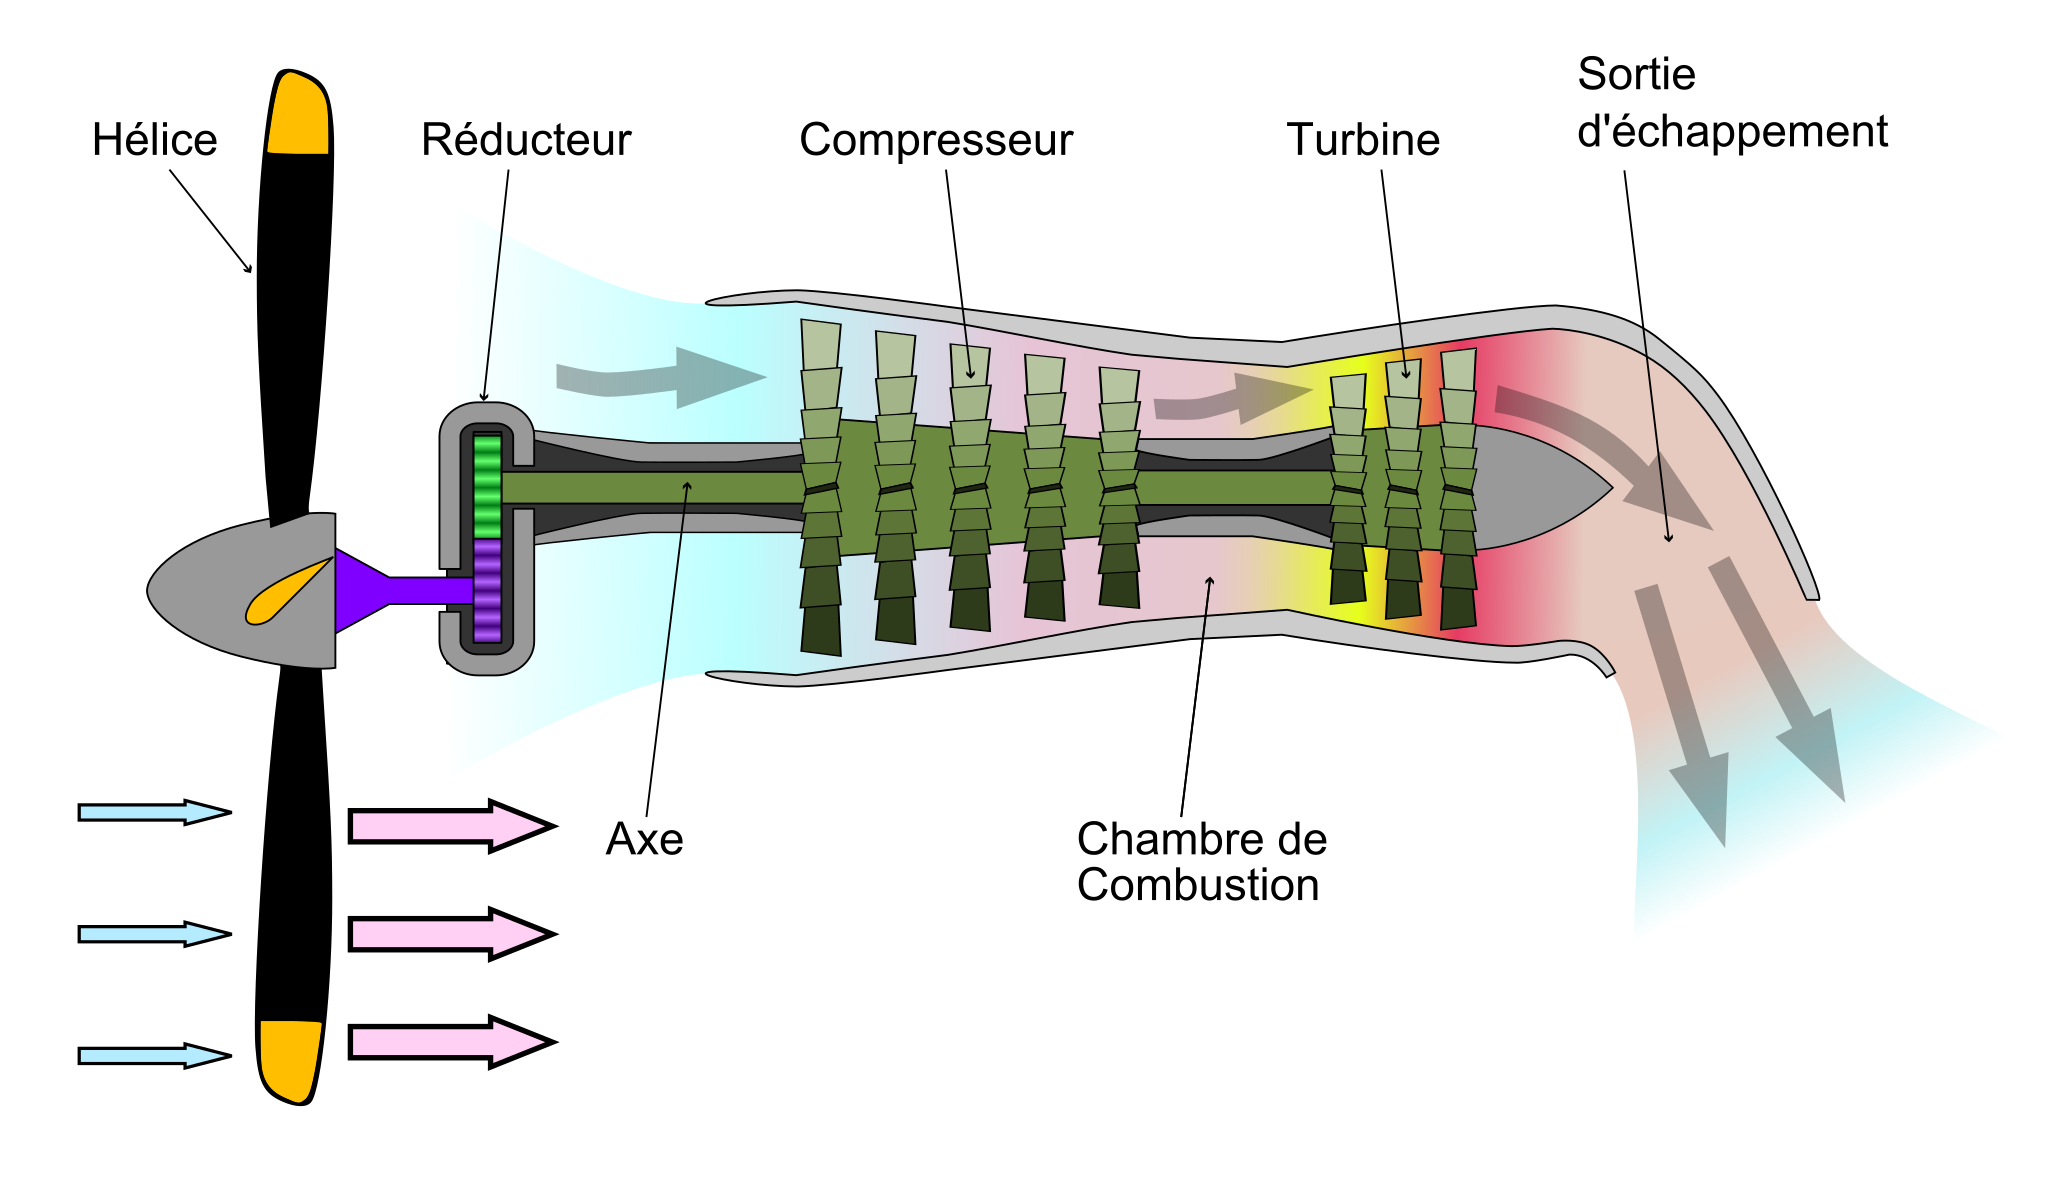
\includegraphics[width=0.75\textwidth]{01-EtudeAeronefs/img/turbomachines/turbopropulseur.pdf}
  	\legende{Schéma d'un turbopropulseur}{img:turbopropulseur}
	\end{figure}	
	
	\subsection{Hélices et moteurs}
	
	\subsection{Propulseurs à réaction}
		\subsubsection{Turboréacteurs}
		
		\begin{figure}[H]
  		\centering
    		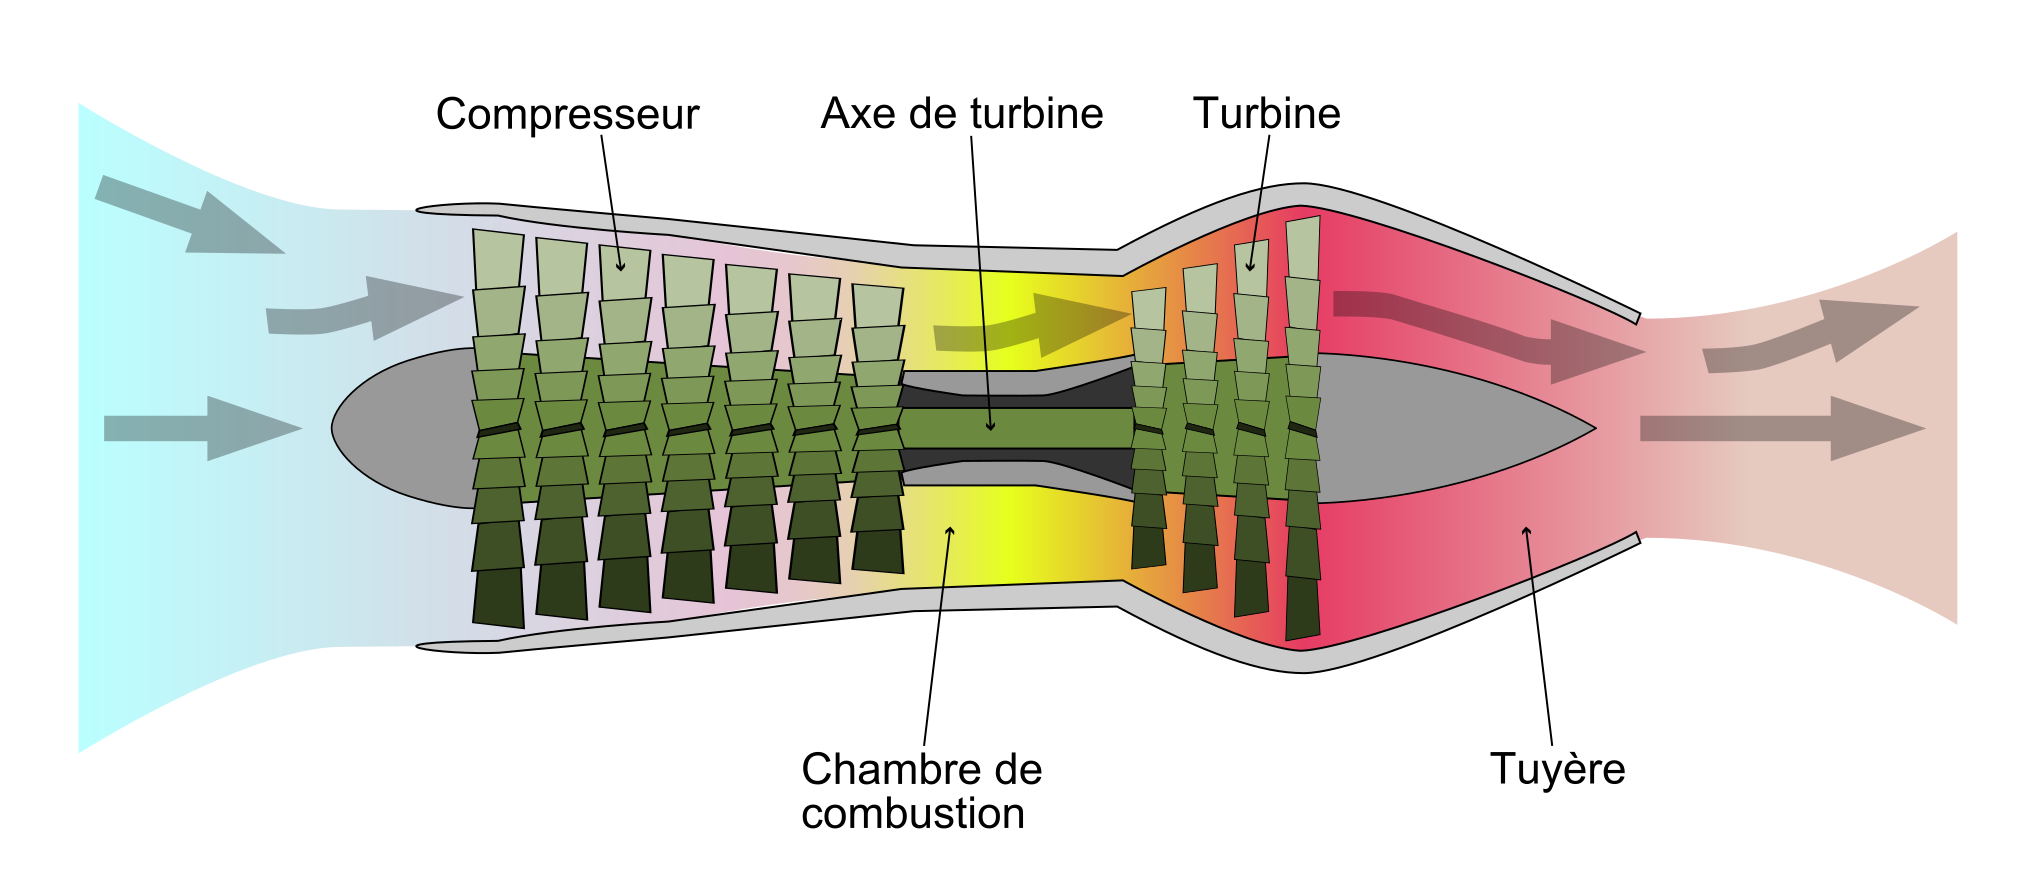
\includegraphics[width=0.75\textwidth]{01-EtudeAeronefs/img/turbomachines/turboreacteur-simpleFlux.pdf}
  		\legende{Schéma d'un turboréacteurs simple flux}{img:turboreacteur-simpleFlux}
		\end{figure}	
	
		\begin{figure}[H]
  		\centering
    		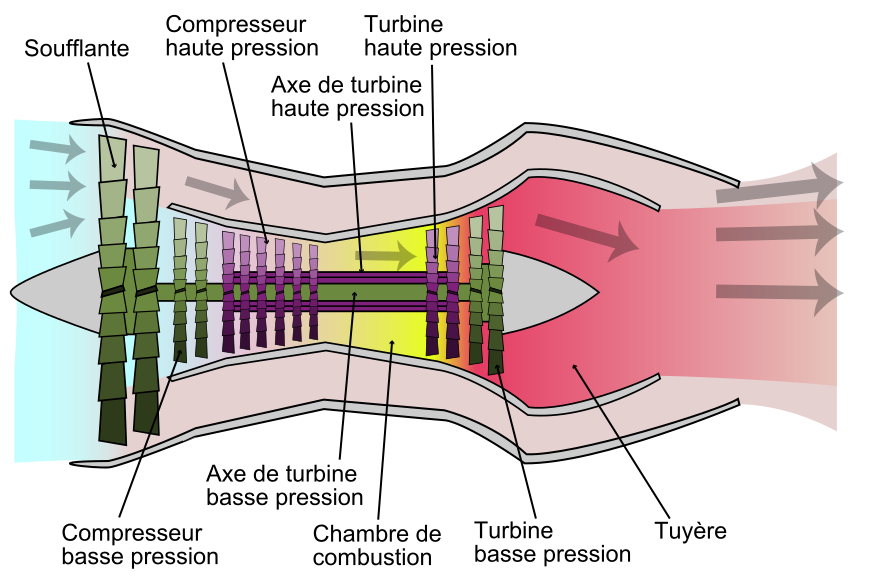
\includegraphics[width=0.75\textwidth]{01-EtudeAeronefs/img/turbomachines/turboreacteur-doubeFlux.pdf}
  		\legende{Schéma d'un turboréacteurs double flux}{img:turboreacteur-doubeFlux}
		\end{figure}	
	
		\subsubsection{Statoréacteurs}
	
		\subsubsection{Moteurs fusées}
		
	\subsection{Contraintes liées au développement durable}

		\section{Structures et matériaux}

%https://fr.wikipedia.org/wiki/Configuration_d%27aile
%https://fr.wikipedia.org/wiki/Profil_(a%C3%A9rodynamique)
%en.wikipedia.org/wiki/Airfoil
%https://fr.wikipedia.org/wiki/Portance_(a%C3%A9rodynamique)
%https://fr.wikipedia.org/wiki/Phare_et_feu_(a%C3%A9ronautique)#:~:text=Ils%20sont%20g%C3%A9n%C3%A9ralement%20situ%C3%A9s%20aux,la%20queue%20de%20l'avion.
%https://en.wikipedia.org/wiki/Drag_(physics)#Aerodynamics


		\section{Les commandes de vol}
	\subsection{Les axes}
	Un aéronef peut bouger sur 3 axes :
	\begin{itemize}
		\item l'axe du roulis \anglais{roll} : il s'agit de l'axe gauche-droite. Cet axe se pilote via les ailerons qui sont actionnés via des mouvements latéraux du manche.
		\item l'axe du tangage \anglais{pitch} : il s'agit de l'axe avant arrière. Cet axe se pilote grâce à la gouverne de profondeur, actionnée via les mouvements longitudinaux du manche. 
		\item l'axe du lacet \anglais{yaw} : il s'agit de l'axe latéral. Cet axe se pilote grâce au gouvernail, actionné grâce aux palonniers.
	\end{itemize}
	
	\begin{figure}[H]
  		\centering
    		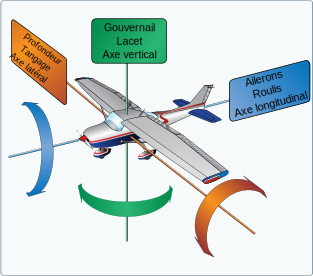
\includegraphics[width=0.6\textwidth]{01-EtudeAeronefs/img/axes.pdf}
  		\legende{Les 3 axes d'un aéronef}{img:axes}
	\end{figure}	
	
	\histoire{On doit à Robert Esnault-Pelterie, ingénieur français, l'invention des ailerons (1905) et du manche à ballet (1906).}
	
	\subsection{Contrôle en roulis}
	Le pilotage en roulis est principalement réalisé grâce à une action sur les ailerons.
	
	Lorsque le pilote actionne le manche d'un côté, l'aileron de l'aile du côté ou le manche est incliné monte, tandis que l'aileron opposé descend. Cela provoque une dissymétrie de portance : la portance augmente du côté ou l'aileron est baissé (même principe qu'un volet), tandis que la portance sur l'aile opposée diminue. En conséquence l'aile avec la surplus de portance monte et la l'aile opposée descend.
	
	\begin{figure}[H]
  		\centering
    		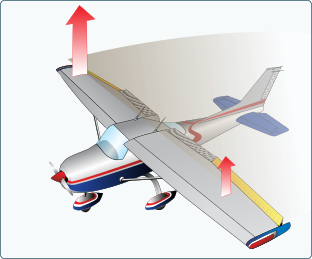
\includegraphics[width=0.6\textwidth]{01-EtudeAeronefs/img/virage.pdf}
  		\legende{Principe de mise en virage par action sur les ailerons}{img:virage}
	\end{figure}	
	
	\subsubsection{Le lacet inverse}
		\begin{figure}[H]
			\centering
  			\includegraphics[width=0.6\textwidth]{01-EtudeAeronefs/img/lacetInverse.pdf}
  			\legende{Lacet inverse (à droite pour un virage à gauche)}{img:lacetInverse}	
		\end{figure}	
	
	\subsection{Contrôle en tangage}
	Le contrôle en tangage est assuré par la gouverne de profondeur.

	La gouverne de profondeur est une surface \textbf{déportante}, c'est à dire qu'elle produit une force inverse en direction inverse des ailes.
		\begin{figure}[H]
			\centering
  			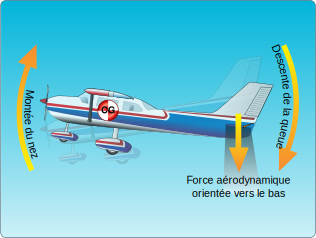
\includegraphics[width=0.6\textwidth]{01-EtudeAeronefs/img/gouverneProfondeur.pdf}
  			\legende{Commande de profondeur}{img:gouverneProfondeur}	
		\end{figure}
		
	\subsection{Le contrôle en lacet}
		\begin{figure}[H]
			\centering
  			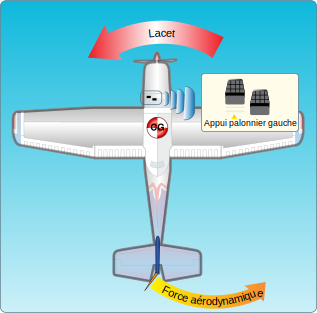
\includegraphics[width=0.6\textwidth]{01-EtudeAeronefs/img/gouverneDeDirection.pdf}
  			\legende{Commande de profondeur}{img:gouverneDeDirection}	
		\end{figure}	
		
		\subsubsection{Le roulis induit}
		
	\subsection{Systèmes de commande de vol}
		\subsubsection{Commandes mécaniques}
		Sur un avion léger, la vitesse faible et la surface limitée des gouvernes, sont actionnables par la seule force du pilote. Pour cela, le manche et le palonnier sont connectés aux gouvernes par un jeu de câble, de poulies de renvoi et de timoneries rigides.
		\begin{figure}[H]
		\centering
  			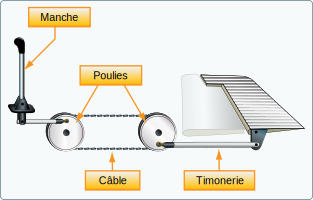
\includegraphics[width=0.6\textwidth]{01-EtudeAeronefs/img/cdvMecaniques.pdf}
  			\legende{Commande de vol mécaniques}{img:cdvMecaniques}	
		\end{figure}	
		
		\subsubsection{Commandes hydrauliques}
		Quand on aéronef devient plus lourd et plus rapide, on augmente la taille des gouvernes pour les rendre plus efficaces. Cette augmentation du flux d'air et la surface plus grande ont une conséquence : les gouvernes deviennent de plus en plus difficiles à man\oe uvrer, jusqu'à un point ou il devient très difficile voir impossible de les faire bouger avec la seule force musculaire des pilotes.
		
		On a donc recours à des systèmes d'assistance hydrauliques. Grâce à de l'huile hydraulique mise en pression grâce à des pompes, des cylindres hydrauliques multiplient la force des pilotes.
		\begin{figure}[H]
		\centering
  			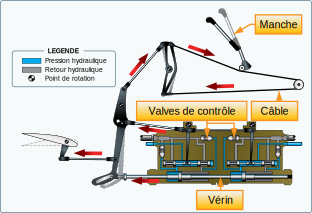
\includegraphics[width=0.55\textwidth]{01-EtudeAeronefs/img/cdvHydrauliques.pdf}
  			\legende{Commande de vol hydrauliques}{img:cdvHydrauliques}	
		\end{figure}	
		Dans ce type de commandes de vol, le manche reste physiquement connecté aux gouvernes de l'avion : en cas de panne du système hydraulique, l'avion reste pilotable, mais cela peut nécessiter une force considérable, voir que les 2 pilotes agissent ensemble sur les commandes.	
		
		Ce type de commande de vol se trouve typiquement sur les avions de ligne du constructeur Boeing.
		
		\subsubsection{Commandes de vol électriques}
		Désormais, certains constructeur ont recours à des commandes de vol dites électriques \anglais{fly-by-wire}. Avec ce type de commande de vol, il n'existe plus aucun lien physique entre les commandes de vol et les gouvernes. Les ordres au manche des pilotes sont convertis en signaux électriques qui sont ensuite traités par des calculateurs (ordinateurs). Ceux ci déterminent les valeurs de positions des gouvernes qui sont alors actionnées par des vérins hydrauliques.
		
		\histoire{Le premier avion de ligne commercial à utiliser des commandes de vol électriques est le Concorde, qui a effectué son premier vol en 1969. \\ En 1984, Airbus effectue le premier vol de l'A320, premier avion de ligne à commandes de vol numériques.}
		
		\info{La totalité de la flotte d'Airbus (sauf A300 et A310) dispose de commandes de vol numériques.}
		
		Les commandes de vol électriques permettent notamment de protéger le domaine de vol de l'avion. Il est par exemple pratiquement impossible de faire décrocher un Airbus : si le pilote agit sur le manche et approche l'incidence de décrochage, le calculateur empêchera la transmission de l'ordre vers les gouvernes.
		%éléments communalisés
\pgfdeclareimage{case}{01-EtudeAeronefs/img/instruments/alt/alt_case.pdf}

\pgfdeclareimage{asiFace}{01-EtudeAeronefs/img/instruments/asi/asi_face.pdf}
\pgfdeclareimage{asiHand}{01-EtudeAeronefs/img/instruments/asi/asi_hand.pdf}
\pgfdeclareimage{asiCase}{01-EtudeAeronefs/img/instruments/asi/asi_case.pdf}

\pgfdeclareimage{altCase}{01-EtudeAeronefs/img/instruments/alt/alt_case.pdf}
\pgfdeclareimage{altFace1}{01-EtudeAeronefs/img/instruments/alt/alt_face_1.pdf}
\pgfdeclareimage{altFace2}{01-EtudeAeronefs/img/instruments/alt/alt_face_2.pdf}
\pgfdeclareimage{altFace3}{01-EtudeAeronefs/img/instruments/alt/alt_face_3.pdf}
\pgfdeclareimage{altHand1}{01-EtudeAeronefs/img/instruments/alt/alt_hand_1.pdf}
\pgfdeclareimage{altHand2}{01-EtudeAeronefs/img/instruments/alt/alt_hand_2.pdf}

\pgfdeclareimage{aiCase}{01-EtudeAeronefs/img/instruments/ai/ai_case.pdf}
\pgfdeclareimage{aiFace}{01-EtudeAeronefs/img/instruments/ai/ai_face.pdf}
\pgfdeclareimage{aiRing}{01-EtudeAeronefs/img/instruments/ai/ai_ring.pdf}
\pgfdeclareimage{aiBack}{01-EtudeAeronefs/img/instruments/ai/ai_back.pdf}

\pgfdeclareimage{hiCase}{01-EtudeAeronefs/img/instruments/hi/hi_case.pdf}
\pgfdeclareimage{hiFace}{01-EtudeAeronefs/img/instruments/hi/hi_face.pdf}

\pgfdeclareimage{tcCase}{01-EtudeAeronefs/img/instruments/tc/tc_case.pdf}
\pgfdeclareimage{tcFace1}{01-EtudeAeronefs/img/instruments/tc/tc_face_1.pdf}
\pgfdeclareimage{tcFace2}{01-EtudeAeronefs/img/instruments/tc/tc_face_2.pdf}
\pgfdeclareimage{tcBall}{01-EtudeAeronefs/img/instruments/tc/tc_ball.pdf}
\pgfdeclareimage{tcBack}{01-EtudeAeronefs/img/instruments/tc/tc_back.pdf}
\pgfdeclareimage{tcMark}{01-EtudeAeronefs/img/instruments/tc/tc_mark.pdf}

\pgfdeclareimage{vsiCase}{01-EtudeAeronefs/img/instruments/vsi/vsi_case.pdf}
\pgfdeclareimage{vsiHand}{01-EtudeAeronefs/img/instruments/vsi/vsi_hand.pdf}
\pgfdeclareimage{vsiFace}{01-EtudeAeronefs/img/instruments/vsi/vsi_face.pdf}

\pgfdeclareimage{ilsCase}{01-EtudeAeronefs/img/instruments/ils/ils_case.pdf}
\pgfdeclareimage{ilsCaseFixed}{01-EtudeAeronefs/img/instruments/ils/ils_case_fixed.pdf}
\pgfdeclareimage{ilsFace}{01-EtudeAeronefs/img/instruments/ils/ils_face.pdf}
\pgfdeclareimage{ilsFlagGs}{01-EtudeAeronefs/img/instruments/ils/ils_flag_gs.pdf}
\pgfdeclareimage{ilsFlagNav}{01-EtudeAeronefs/img/instruments/ils/ils_flag_nav.pdf}
\pgfdeclareimage{ilsHandGs}{01-EtudeAeronefs/img/instruments/ils/ils_hand_gs.pdf}
\pgfdeclareimage{ilsHanvNav}{01-EtudeAeronefs/img/instruments/ils/ils_hand_nav.pdf}

%altimètre
%   -paramètre 1 : altitude en pieds
%   -paramètre 2 : calage en pouces de mercure
\def\alti#1#2{
	\fill[transparent] (0,0) circle (3) ;
	\node[rotate=(#2-28.0)*100] {\pgfbox[center,center]{\pgfuseimage{altFace1}}};
	\node {\pgfbox[center,center]{\pgfuseimage{altFace2}}};
  	\node[rotate=-{(Mod(#1/10,10000))*(36/1000)}] {\pgfbox[center,center]{\pgfuseimage{altFace3}}};
  	\node[rotate=-{(Mod(#1,1000))*(360/1000)}] {\pgfbox[center,center]{\pgfuseimage{altHand2}}};
    	\node[rotate=-{(Mod(#1,10000))*(360/10000)}] {\pgfbox[center,center]{\pgfuseimage{altHand1}}};
    	%\node {\pgfbox[center,center]{\pgfuseimage{altCase}}};
	\node {\pgfbox[center,center]{\pgfuseimage{case}}};
}

%consevateur de cap
%   -paramètre 1 : cap en degrés
\def\conservateurCap#1{
	\fill[transparent] (0,0) circle (3) ;
  	\node[rotate=#1] {\pgfbox[center,center]{\pgfuseimage{hiFace}}};
    	\node {\pgfbox[center,center]{\pgfuseimage{hiCase}}};
}

%ILS
%   -paramètre 1 : QDM en degrés
%   -paramètre 2 : décallage horizontal
%   -paramètre 3 : décallage vertical
\pgfkeys{
    /ilsparam/.is family,
    /ilsparam,
    qdm/.store in = \ilsQdm,
    ecartLoc/.store in = \ilsEcartLoc,
    ecartGlide/.store in = \ilsEcartGlide,
    afficherFlagNav/.store in = \ilsAfficherFlagNav,
    afficherFlagGs/.store in = \ilsAfficherFlagGs,
    qdm = 0,
    ecartLoc = 0,
    ecartGlide = 0,
    afficherFlagNav = false,
    afficherFlagGs = false,
}
\newcommand{\ils}[1]{
    \pgfkeys{/ilsparam, #1}
%\def\ils#1#2#3{
	\fill[transparent] (0,0) circle (3) ;
		\node {\pgfbox[center,center]{\pgfuseimage{ilsCaseFixed}}};
		\ifthenelse{\equal{\ilsAfficherFlagGs}{true}}{
			\node {\pgfbox[center,center]{\pgfuseimage{ilsFlagGs}}};
		}
		\ifthenelse{\equal{\ilsAfficherFlagNav}{true}}{
			\node {\pgfbox[center,center]{\pgfuseimage{ilsFlagNav}}};
		}
		\node[yshift=\ilsEcartGlide*31.75] {\pgfbox[center,center]{\pgfuseimage{ilsHandGs}}};
		\node[xshift=\ilsEcartLoc*31.75] {\pgfbox[center,center]{\pgfuseimage{ilsHanvNav}}};
		\node[rotate=\ilsQdm] {\pgfbox[center,center]{\pgfuseimage{ilsFace}}};
    	\node {\pgfbox[center,center]{\pgfuseimage{ilsCase}}};
}

%variomètre
%   -paramètre 1 : taux de descente
\def\vario#1{
	\fill[transparent] (0,0) circle (3) ;
  	\node {\pgfbox[center,center]{\pgfuseimage{vsiFace}}};
   	\node[rotate=-(#1/2000)*172] {\pgfbox[center,center]{\pgfuseimage{vsiHand}}};
    	%\node {\pgfbox[center,center]{\pgfuseimage{vsiCase}}};
	\node {\pgfbox[center,center]{\pgfuseimage{case}}};
}

%horizon
%   -paramètre 1 : roulis
%   -parametre 2 : tangage 
\def\horizon#1#2{
	\fill[transparent] (0,0) circle (3) ;
	\node {\pgfbox[center,center]{\pgfuseimage{aiBack}}};
  	\node[rotate=#1,yshift=-#2*1.25] {\pgfbox[center,center]{\pgfuseimage{aiFace}}};
    	\node[rotate=#1] {\pgfbox[center,center]{\pgfuseimage{aiRing}}};
    	\node {\pgfbox[center,center]{\pgfuseimage{aiCase}}};
}

%indicateur de virage
%   -paramètre 1 : taux virage [-1;1] 
%   -parametre 2 : postion bille [-1;1] 
\def\indicateurVirage#1#2{
	\fill[transparent] (0,0) circle (3) ;
  	\node {\pgfbox[center,center]{\pgfuseimage{tcBack}}};
    	\node {\pgfbox[center,center]{\pgfuseimage{tcFace1}}};
    	\node {\pgfbox[center,center]{\pgfuseimage{tcFace2}}};
    	%\node[xshift=#2*35,yshift=#2*4] {\pgfbox[center,center]{\pgfuseimage{tcBall}}};
	\node[rotate around={#2*15:(0,3.7)}] {\pgfbox[center,center]{\pgfuseimage{tcBall}}};
    	\node[rotate=#1*20] {\pgfbox[center,center]{\pgfuseimage{tcMark}}};
    	%\node {\pgfbox[center,center]{\pgfuseimage{tcCase}}};
	\node {\pgfbox[center,center]{\pgfuseimage{case}}};
}

%badin
%   -paramètre 1 : vitesse [0;200] 
\def\badin#1{
	\fill[transparent] (0,0) circle (3) ;
  	\node {\pgfbox[center,center]{\pgfuseimage{asiFace}}};
    	
	%0 kts : 0°
	%40 kts : 36°
	%70 kts : 90°
	%130 kts : 210°
	%160 kts : 264°
	%200 kts : 312°

	%	Vitesse	Position aiguille	Angle/10 kts
	%	0		0,00°	
	%	40		36,00°		NA
	%	50		54,00°		-18°
	%	60		72,00°		-18°
	%	70		90,00°		-18°
	%	80		110,00°		-20°
	%	90		130,00°		-20°
	%	100		150,00°		-20°
	%	110		170,00°		-20°
	%	120		190,00°		-20°
	%	130		210,00°		-20°
	%	140		228,00°		-18°
	%	150		246,00°		-18°
	%	160		264,00°		-18°
	%	200		312,00°		-12°

	%Entre 0 et 40 kts
	\ifnum#1<41
	\node[rotate=-(((#1)/(40))*(36))] {\pgfbox[center,center]{\pgfuseimage{asiHand}}};
	\fi 
	%Entre 40 et 70 kts
	\ifnum#1>40 \ifnum#1<71
	\node[rotate=-(((#1-40)/(70-40))*(90-36))-36] {\pgfbox[center,center]{\pgfuseimage{asiHand}}};
	\fi \fi
	%Entre 71 et 130 kts
	\ifnum#1>70 \ifnum#1<131
	\node[rotate=-(((#1-70)/(130-70))*(210-90))-90] {\pgfbox[center,center]{\pgfuseimage{asiHand}}};
	\fi \fi
	%Entre 130 et 160 kts
	\ifnum#1>130 \ifnum#1<161
	\node[rotate=-(((#1-130)/(160-130))*(264-210))-210] {\pgfbox[center,center]{\pgfuseimage{asiHand}}};
	\fi \fi
	%Entre 160 et 200 kts
	\ifnum#1>160
	\node[rotate=-(((#1-160)/(200-160))*(312-264))-264] {\pgfbox[center,center]{\pgfuseimage{asiHand}}};
	\fi

    	%\node {\pgfbox[center,center]{\pgfuseimage{asiCase}}};
	\node {\pgfbox[center,center]{\pgfuseimage{case}}};
}

% Définir les clés pour les paramètres
\pgfkeys{
    /tdb/.is family,
    /tdb,
    vitesse/.store in = \tdbVitesse,
    altitude/.store in = \tdbAltitude,
    calageAltitude/.store in = \tdbCalageAltitude,
    vz/.store in = \tdbVz,
    cap/.store in = \tdbCap,
    assiette/.store in = \tdbAssiette,
    inclinaison/.store in = \tdbInclinaison,
    derapage/.store in = \tdbDerapage,
    virage/.store in = \tdbVirage,
    afficherT/.store in = \tdbAfficherT,
    vitesse = 0,
    altitude = 0,
    vz = 0,
    cap = 0,
    assiette = 0,
    inclinaison = 0,
    derapage = 0,
    virage = 0,
    calageAltitude = 30,
    afficherT = false,
}

%Planche de bord
\newcommand{\dessinerTdB}[1]{
    \pgfkeys{/tdb, #1}

    \begin{tikzpicture}
        % Définir les coordonnées des sommets de la planche de bord
        \coordinate (A) at (-5, 3.5);
        \coordinate (B) at (19, 3.5);
        \coordinate (C) at (19, -10.5);
        \coordinate (D) at (-5, -10.5);

        % Dessiner le polygone avec le coin supérieur gauche arrondi
        \fill[gray, rounded corners=3cm] (D) -- (A) -- (B) -- (C) -- cycle ;

        % Dessiner le polygone rouge si showredpolygon est vrai
        \ifthenelse{\equal{\tdbAfficherT}{true}}{
            \coordinate (T1) at (-3.2, 3.2);
            \coordinate (T2) at (17.2, 3.2);
            \coordinate (T3) at (17.2, -3.5);  
            \coordinate (T4) at (10.4, -3.5);
            \coordinate (T5) at (10.4, -10.2);
            \coordinate (T6) at (3.6, -10.2);
            \coordinate (T7) at (3.6, -3.5); 	
            \coordinate (T8) at (-3.2, -3.5); 
            \draw[line width=5pt, red] (T1) -- (T2) -- (T3) -- (T4) -- (T5) -- (T6) -- (T7) -- (T8) -- cycle  ;
        }{}

        % Placer les instruments
        \begin{scope}[xshift=0cm, yshift=0cm]
            \badin{\tdbVitesse}
        \end{scope}
        
        \begin{scope}[xshift=7cm, yshift=0cm]
            \horizon{\tdbInclinaison}{\tdbAssiette}
        \end{scope}
        
        \begin{scope}[xshift=14cm, yshift=0cm]
            \alti{\tdbAltitude}{\tdbCalageAltitude}
        \end{scope}
        
        \begin{scope}[xshift=0cm, yshift=-7cm]
            \indicateurVirage{\tdbVirage}{\tdbDerapage}
        \end{scope}
        
        \begin{scope}[xshift=7cm, yshift=-7cm]
            \conservateurCap{\tdbCap}
        \end{scope}
        
        \begin{scope}[xshift=14cm, yshift=-7cm]
            \vario{\tdbVz}
        \end{scope}

        %\draw (B) grid (D);    
        
    \end{tikzpicture}
}



\section{L'instrumentation de bord}
	\subsection{L'indicateur de vitesse}

	\begin{figure}[H]	
	\centering
	\begin{tikzpicture}
	\fill[transparent] (0,0) circle (3) ;
  	\node {\pgfbox[center,center]{\pgfuseimage{asiFace}}};
    \node[rotate=-45] {\pgfbox[center,center]{\pgfuseimage{asiHand}}};
    \node {\pgfbox[center,center]{\pgfuseimage{asiCase}}};
	\end{tikzpicture}
	\end{figure}
	
	\subsection{L'altimètre}
	
	\begin{figure}[H]	
	\centering
	\begin{tikzpicture}
	\fill[transparent] (0,0) circle (3) ;
	\node {\pgfbox[center,center]{\pgfuseimage{altFace1}}};
	\node {\pgfbox[center,center]{\pgfuseimage{altFace2}}};
  	\node {\pgfbox[center,center]{\pgfuseimage{altFace3}}};
  	\node[rotate=-30] {\pgfbox[center,center]{\pgfuseimage{altHand2}}};
    \node[rotate=-45] {\pgfbox[center,center]{\pgfuseimage{altHand1}}};
    \node {\pgfbox[center,center]{\pgfuseimage{altCase}}};
	\end{tikzpicture}
	\end{figure}
	
	\subsection{L'horizon artificiel}
	
	\begin{figure}[H]	
	\centering
	\begin{tikzpicture}
	\fill[transparent] (0,0) circle (3) ;
	\node {\pgfbox[center,center]{\pgfuseimage{aiBack}}};
  	\node[rotate=0] {\pgfbox[center,center]{\pgfuseimage{aiFace}}};
    \node[rotate=0] {\pgfbox[center,center]{\pgfuseimage{aiRing}}};
    \node {\pgfbox[center,center]{\pgfuseimage{aiCase}}};
	\end{tikzpicture}
	\end{figure}
	
	\subsection{Le conservateur de cap}
	
	\begin{figure}[H]	
	\centering
	\begin{tikzpicture}
	\fill[transparent] (0,0) circle (3) ;
  	\node[rotate=0] {\pgfbox[center,center]{\pgfuseimage{hiFace}}};
    \node {\pgfbox[center,center]{\pgfuseimage{hiCase}}};
	\end{tikzpicture}
	\end{figure}
	
	
	\subsection{L'indicateur de virage}
	
	\begin{figure}[H]	
	\centering
	\begin{tikzpicture}
	\fill[transparent] (0,0) circle (3) ;
  	\node {\pgfbox[center,center]{\pgfuseimage{tcBack}}};
    \node {\pgfbox[center,center]{\pgfuseimage{tcFace1}}};
    \node {\pgfbox[center,center]{\pgfuseimage{tcFace2}}};
    \node {\pgfbox[center,center]{\pgfuseimage{tcBall}}};
    \node {\pgfbox[center,center]{\pgfuseimage{tcMark}}};
    \node {\pgfbox[center,center]{\pgfuseimage{tcCase}}};
	\end{tikzpicture}
	\end{figure}
	
	
	\subsection{Le variomètre}
	
	\begin{figure}[H]	
	\centering
	\begin{tikzpicture}
	\fill[transparent] (0,0) circle (3) ;
  	\node {\pgfbox[center,center]{\pgfuseimage{vsiFace}}};
    \node[rotate=0] {\pgfbox[center,center]{\pgfuseimage{vsiHand}}};
    \node {\pgfbox[center,center]{\pgfuseimage{vsiCase}}};
	\end{tikzpicture}
	\end{figure}
	
	\chapter{Navigation, réglementation, sécurité des vols}
	\label{nav}
		\section{Navigation}
	\subsection{Les grands principes de navigation}
		\subsubsection{Navigation à l'estime et cheminement à vue}
		\subsubsection{Route vraie, route magnétique, cap vrai, cap magnétique, déclinaison, déviation}
		\subsubsection{Distance entre deux points d'une carte}
		\subsubsection{Régimes de vol}
		Un aéronef évolue toujours selon des règles partagées. Pour les vols civils, on dit que l'on évolue selon les règles de la \textbf{\acrlong{cag}}	(\acrshort{cag}). La CAG défini 2 grandes régimes de vol : le VFR et l'IFR.\\
		
		Il existe d'autres règles de circulation aérienne, on peut citer par exemple la CAM (Circulation Aérienne Militaire) ou encore la CER (Circulation d'Essais et de Réception). Ces circulations ne seront pas abordées ici.
		
		\paragraph{Le vol à vue}
		Le vol \acrshort{vfr} (\anglais{\acrlong{oaci}} - règles de vol à vue) correspond historiquement au premier mode de navigation utilisé pour se déplacer en avion. Dans ce mode de navigation, on navigue principalement grâce à des repères au sol, et on pilote l'attitude de l'avion grâce a l'horizon naturel. 
		
		L'instrumentation minimale pour ce type de vol est très réduite. On peut naviguer aisément en VFR avec seulement un anémomètre (pour connaitre sa vitesse), une boussole (pour connaitre son cap) et une montre (pour mesurer le temps avant d'atteindre le prochain point de repère de la navigation), même si aujourd'hui les appareils exploités en VFR sont généralement équipés d'une instrumentation bien plus élaborée.
		
		\astuce{En français, on dit parfois VFR peut être traduit par \textbf{Voies-Ferrées/Routes} car pour naviguer selon les règles VFR on utilise des repères au sol, dont les routes et les voies ferrées.}
		
		Le principal inconvénient de ce mode de navigation est qu'il nécessite que les conditions météo soient suffisamment bonnes pour que l'horizon demeure visible et que les points de repères au sol soient identifiables. Ce régime de vol n'est donc utilisable que par beau temps. Les conditions de vols requises pour le vol VFR sont appelées \acrshort{vmc} (\anglais{\acrlong{vmc}} - conditions de vol à vue). Les conditions VMC définissent des visibilité horizontales et des distance par rapport aux nuages minimales permettant de voler à vue. Ces valeurs minimales dépendent de l'espace ou l'aéronef évolue.
		
		\info{Il est possible de voler selon les règles VFR la nuit, on parle alors de NVFR \anglais{Night VFR}.}
		
		\info{Il est possible de se servir des instruments de radionavigation ou du GPS pour naviguer en VFR, toujours en gardant les conditions VMC.}
		
		Aujourd'hui, ce mode de navigation reste très utilisée pour l'aviation de loisir mais également pour bon nombre de missions professionnelles (évacuations sanitaires, héliportage, surveillance d'infrastructures, largages de parachutistes...). \\
		
		Pour offrir des capacités de vol par conditions météo dégradées, il a donc fallu inventer un autre régime de vol : l'IFR.
		
		\paragraph{Le vol aux instruments}
		Le vol \acrshort{ifr} (\anglais{\acrlong{ifr}} - règles de vol aux instruments) définis les règles et procédure permettant de voler par tout temps, lorsque les conditions \acrshort{vmc} ne sont plus réunies. On se trouve alors en conditions \acrshort{imc}(\anglais{\acrlong{imc}} - conditions de vol aux instruments).
		
		Dans ces conditions, les informations visuelles obtenues par le sens du pilote (essentiellement la vue) ne permettent plus de piloter l'attitude de l'avion (absence d'horizon naturel) ni de naviguer (les repères au sol tout comme les obstacles sont cachés par la mauvaise visibilité, et deviennent invisibles ou visibles trop tardivement). Dans ces conditions, les pilotes vont donc se baser sur des références instrumentales pour le pilotage :
		\begin{itemize}
		\item horizon artificiel pour piloter l'attitude de l'appareil,
		\item radiobalises, guidage radar ou plus récemment GPS pour la navigation.
		\end{itemize}
		
		On constate que cette règle de navigation nécessite une instrumentation plus élaborée. Par ailleurs, il est nécessaire que l'avion et le pilote soient qualifiés pour l'IFR. Si on souhaite se poser sur un aéroport en conditions IMC, il faut également que cet aéroport soit qualifié pour l'IFR.
		
		\info{Un aéronef qui évolue selon les règles \acrshort{ifr} peut évoluer en conditions \acrshort{vmc}.}
		
		\info{Bien que la plupart des vols soient menés selon un seul régime de vol, il est cependant possible de changer de régime de vol durant le vol, sous réserve que l'avion, le pilote et éventuellement l'aéroport soient qualifiés pour l'IFR. Il est par exemple possible de réaliser le décollage et la croisière en VFR, puis de passer en IFR à l'arrivée si les conditions à l'aéroport de destination sont IMC.}
		
		\paragraph{Le VFR spécial} 
		Il existe un régime de vol particulier appelé VFR Spécial. Ce régime de vol n'est possible qu'en espace aérien contrôlé. Ce régime de vol permet d'abaisser les conditions de vol VMC en espace aérien contrôlé.
		
		\exemple{Pour évoluer dans une CTR de classe D, les conditions VMC exigent 5000~m de visibilité et de conserver 300~m d'espacement vertical et 1500~m d'espacement horizontal avec les nuages. Un pilote qui évoluerait en espace de classe D avec 4000~m de visibilité serait donc en conditions IMC. En passant en VFR spécial, les conditions météo peuvent être ramenées à 1500~m de visibilité et hors des nuages.}
		
		Le VFR spécial est soumis à \textit{clearance} du contrôle aérien. La délivrance de la \textit{clearance} impose alors au contrôleur d'assurer la séparation entre le vol VFR spécial et les vols IFR.
		
	
	\subsection{Les outils de navigation}
		\subsubsection{Cartes aéronautiques}
		
		\subsubsection{Aides à la navigation}
			\paragraph{Notions de base}
			
			\paragraph{Le VOR}
			
			\subparagraph{Le VOR-DME}
			
			\paragraph{L'ADF}
			
			\paragraph{Le GPS}
		\section{Réglementation aéronautique}
	\subsection{L'organisation de l'espace aérien}
	Afin de permettre aux aéronefs d'évoluer en toute sécurité, l'espace aérien a été divisé en différents espaces, qui présentent chacun des conditions d'accès spécifiques et des services associés.
		
		\subsubsection{Les classes d'espaces aériens}
		Au niveau mondial, l'OACI à définit 7 classes d'espaces aériens, nommées par des lettres de A (classe présentant le plus de contraintes) à G (classe présentant le moins de contraintes). Dans ce chapitre, nous allons voir quelles sont les différences entre ces classes.
		
		\paragraph{Classe A}
		
		\paragraph{Classe B}
		
		\paragraph{Classe C}
		
		\paragraph{Classe D}\label{classeD}
		
		\paragraph{Classe E}
		
		\paragraph{Classe F}
		
		\paragraph{Classe G}
		
		\subsubsection{Les zones à statut particulier}
			\paragraph{Les zones R}
			Les zones R sont des zones \textbf{R}estreintes. La pénétration de ces zones est possible sous condition. Par exemple, \hyperlink{ignOaciBordeaux.1}{sur la carte extrait de Bordeaux (cf \ref{ignOaciBdx} page \pageref{ignOaciBdx})}, on peut entrer dans la zone R~204~L3 si on est en contact avec le service d'information de vol Aquitaine Info\footnote{Source : extrait de l'ENR5.1 "VFR : pénétration après contact radio avec AQUITAINE INFO. Veille radio obligatoire."}.
			
			Ces zones peuvent être actives en permanence ou seulement sur certaines tranches horaire.
			
			\paragraph{Les zones D}
			Les zone D sont des zones \textbf{D}angereuses. Leur pénétration n'est pas formellement interdite mais les activités qui s'y déroulent sont suffisamment risquées pour qu'il existe une nécessité d'avertir les navigateurs aériens. Pour ces zones, on dispose généralement d'un organisme à contacter par radio pour connaitre l'activité réelle.
			
			\alert{Il ne faut pas confondre les zones D avec les espaces aériens de classe D (cf \ref{classeD} page \pageref{classeD}}.
			
			Ces zones peuvent être actives en permanence ou seulement sur certaines tranches horaire.
			
			\paragraph{Les zones P}
			Les zones P sont des zones interdites (\textbf{P}rohibées). Le vol dans ces zones est en général strictement interdit. En France, ces zones protègent généralement des infrastructures critiques, comme des centrales nucléaires. Par exemple, \hyperlink{ignOaciBordeaux.1}{sur la carte extrait de Bordeaux (cf \ref{ignOaciBdx} page \pageref{ignOaciBdx})}, la zone P~5 protège les installations du laser mégajoule au Barp. Cette zone est interdit de pénétration sauf pour les vols IFR ayant obtenu l'autorisation du contrôle, les vols de secours qui ne peuvent contourner dans le cadre de leur missions, et les aéronefs spécifiquement autorisés\footnote{Source : ENR 5.1 1.2.1}.
			
			Ces zones sont généralement actives en permanence.
	
	\subsection{Titres aéronautiques}
	
	\subsection{Les organisations}
	
	\subsection{Contrôle d'un aéronef}
		\section{Sécurité des vols}
	\subsection{Gestion des risques}
	
	\subsection{Performances humaines et ses limites}
	
	\subsection{Prise de décision}
	
	\ifdefined\activerrelease 
	\else
	\chapter{Météorologie et aérologie}
	\label{meteo}
		\section{L'atmospère}
	L'atmosphère terrestre est la mince couche de gaz qui entoure la Terre.
	
	On considère que l'atmosphère à une épaisseur d'environ 120 km, hauteur à laquelle le ralentissement lié à l'atmosphère devient notable.
	\subsection{Composition}
	
	L'atmosphère est composée d'un ensemble de gaz dont la proportion est constante pratiquement dans toutes l'atmosphère. Cet ensemble de gaz est appelé \textbf{air}. Un autre gaz, la vapeur d'eau, est souvent mélangé à cet air, en proportion variable selon le temps, le lieu et l'altitude. La proportion de vapeur d'eau que peut contenir l'air va jusqu'à environ 5~\%.
	
	L'air sec est composé de :
	\begin{table}[H]
	\centering
	\begin{tabular}{|l|c|}
		\hline
		Gaz & Proportion \\
		\hline
		\hline
		Azote ($N$) & 78~\% \\
		\hline
		Oxygène ($O$) & 21~\% \\
		\hline
		Argon ($Ar$) & 0,9~\% \\
		\hline
		Autres gaz (dont Dioxyde de carbone ($CO_2$)) & 0,1~\% \\
		\hline
	\end{tabular}
	\caption{Composition de l'atmosphère terrestre}
	\end{table}
	
	
	\subsection{Structure}
	L'atmosphère a été découpée en plusieurs couches successives, dont les limites ont été fixées sur la base des discontinuités des variations de température que l'on y rencontre.
	
	\begin{figure}[H]
			\centering
			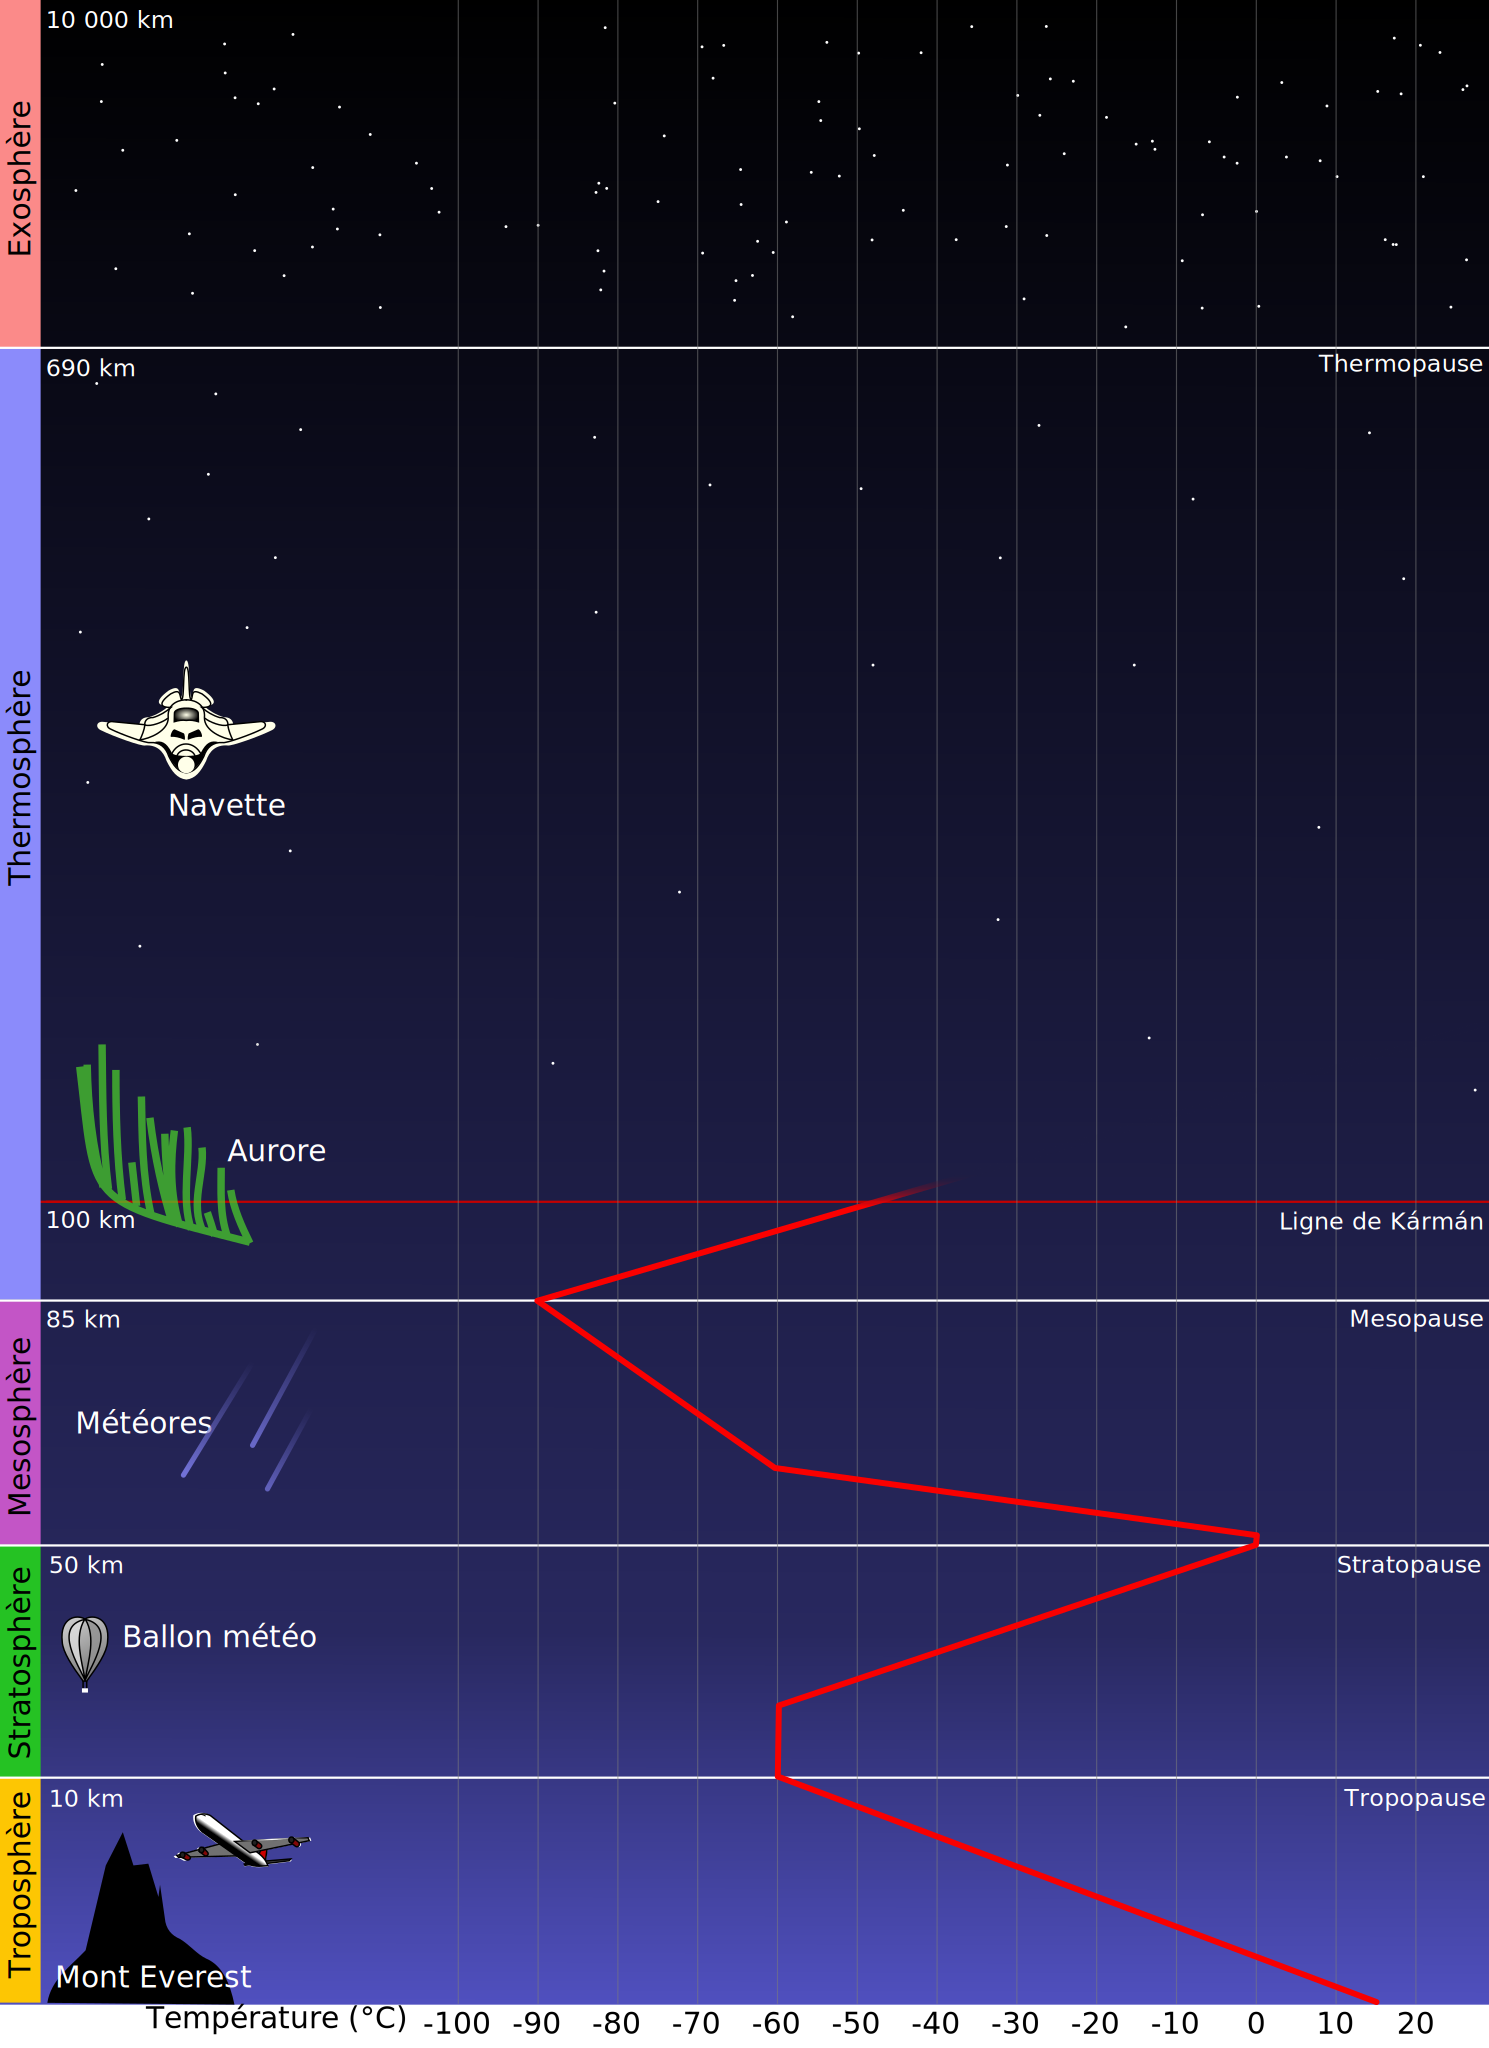
\includegraphics[width=0.8\linewidth]{03-Meteo/img/couchesAtmosphereTemperature.pdf}
			\legende{Schéma des couches de l'atmosphère, avec la courbe de température normale et le nom des limites}{img:couchesAtmosphereTemperature}
			\end{figure}	
			
	\subsection{La pression atmosphérique}
	La colonne d'air qui se trouve au dessus de nos têtes subit la gravité terrestre. Par conséquence, elle représente un poids, appelé pression atmosphérique.
	
	Cette pression peut-être mise en évidence grâce à des baromètres, des dispositifs prévus pour mesurer la valeur de cette pression.
	
	Cette pression a été mise en évidence par le physicien italien Evangelista Torricelli au début du \siecle{17}. Le physicien rempli un tube en verre fermé d'un côté avec du mercure, puis le retourne dans une cuve elle aussi remplie de mercure. Dans le tube, le mercure descend et se stabilise à une hauteur de 760 mm.
	
	\begin{figure}[H]
	\centering
	\begin{tikzpicture}[scale=1.7, every node/.style={scale=1.7}]
	\barometreTorricelli{760} 
	\draw [line width=0.5mm, -{Stealth[length=10mm, open, round]}]
          (-1,2) -- (-1,0.7);
    \draw [line width=0.5mm, -{Stealth[length=10mm, open, round]}]
          (1,2) -- (1,0.7);
	\end{tikzpicture}
	\legende{Baromètre de Torricelli au mercure, au niveau de la mer}{img:barometreTorricelli}
	\end{figure}
	
	La pression atmosphérique appuie en réalité sur le mercure contenu dans la cuve.
	
	\subsubsection{Variation de la pression atmosphérique avec l'altitude}
	Lorsque l'on se déplace verticalement dans l'atmosphère, la colonne d'air qui se trouve au dessus est moins haute. Par conséquence, la pression atmosphérique diminue lorsque l'on s'élève dans l'atmosphère.
	
	\begin{figure}[H]
		\ifdefined\activeranimations 
		\newcommand{\nbFramesAltitude}{101}
		\else
		\newcommand{\nbFramesAltitude}{1}
		\fi
		
		%760 mmHg à 0 m
		%200 mmHg à 10 000 m
		%=> 560 mmHg entre les 2, soit, pour 100 frames, 5.6
		%\newcommand{\altToMmHg}{((760-200)/\nbFramesAltitude)}
		%\newcommand{\altToMmHg}{0.2}
		
		\centering
		\begin{animateinline}[controls,loop]{8}
		    \multiframe{\nbFramesAltitude}{i=0+1}{
			\begin{tikzpicture}[x=1cm,y=1cm, scale=0.5, every node/.style={scale=0.5}]
				\echelleAltitudeMetres{10}{\i/10}
			\end{tikzpicture}
			\begin{tikzpicture}[scale=1.1, every node/.style={scale=1.1}]
				%\FPeval{\asoustraire}{clip(\i*\altToMmHg)}
				\FPeval{\result}{round((760-\i*5.6),0)}
				\barometreTorricelli{\result}		
			\end{tikzpicture}
			}
		\end{animateinline}
	\end{figure}
		\section{Les nuages}
	Un nuage est une masse visible dans l'atmosphère. Ils sont constitués de gouttelettes d'eau (liquide ou sous forme de cristaux de glace) en suspension dans l'air.
	
	Les nuages peuvent présenter des dangers pour l'activité aéronautique :
	\begin{itemize}
		\item réduction de la visibilité pour les nuages proches du sol ou lorsqu'ils sont pénétrés en vol,
		\item problématiques liées aux précipitations ou aux vents qu'ils génèrent,
		\item phénomènes de givrage cellule lié à l'humidité présente dans les nuages.
\end{itemize}

	L'identification des grandes familles de nuages et la connaissance des risques associés à chacune d'entre elles est donc nécessaire.
	
    \begin{figure}[H]
    \centering
    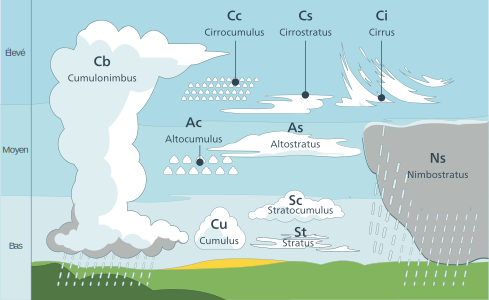
\includegraphics[width=0.75\textwidth]{03-Meteo/img/nuages.pdf}
    \legende{Répartition des types de nuages dans la troposphère}{img:nuages}
    \end{figure}	
		\section{Les masses d'air et les fronts}
	\subsection{Les masses d'air}
		\subsubsection{Anticyclones}
		\subsubsection{Dépressions}
		\subsubsection{Cols, dorsales, talwegs et marais barométriques}
	\subsection{Les fronts}
	
		\begin{figure}[H]
			\centering
			\includegraphics[width=0.85\linewidth]{03-Meteo/img/frontIsobares20260127.png}
			\legende{Carte des isobares}{img:frontIsobares20260127}
		\end{figure}	
		
		\begin{figure}[H]
			\centering
			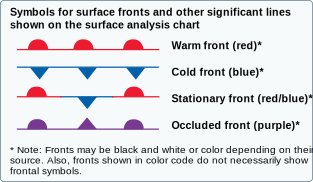
\includegraphics[width=0.4\linewidth]{03-Meteo/img/legendeFronts.pdf}
			\legende{Symboles des fronts sur une carte météorologique}{img:legendeFronts}
		\end{figure}	
	
	
		\subsubsection{Front froid}
		\begin{figure}[H]
			\centering
			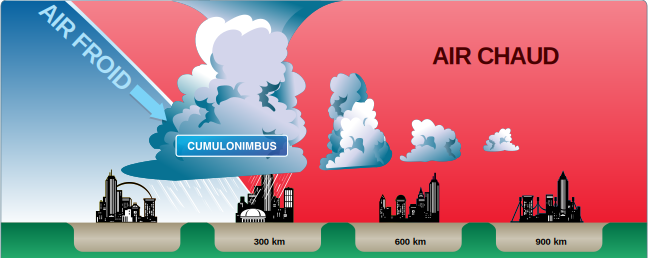
\includegraphics[width=0.75\linewidth]{03-Meteo/img/frontFroid.pdf}
			\legende{Coupe d'un front froid}{img:frontFroid}
		\end{figure}	
		
		
		\subsubsection{Front chaud}
		\begin{figure}[H]
			\centering
			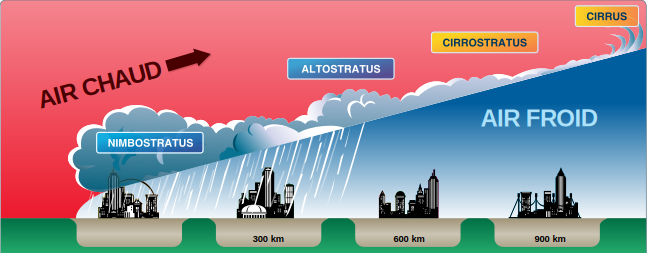
\includegraphics[width=0.75\linewidth]{03-Meteo/img/frontChaud.pdf}
			\legende{Coupe d'un front chaud}{img:frontChaud}
		\end{figure}	
		
		
		\subsubsection{Front occlus}
		\begin{figure}[H]
			\centering
			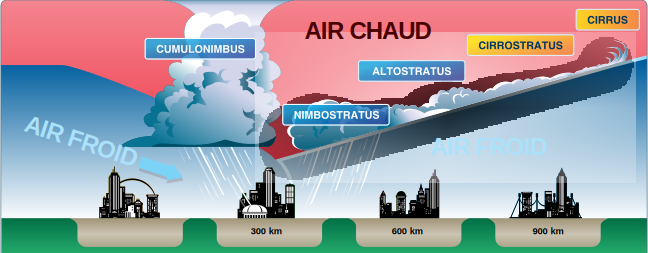
\includegraphics[width=0.75\linewidth]{03-Meteo/img/frontOcclus.pdf}
			\legende{Coupe d'un front occlus}{img:frontOcclus}
		\end{figure}		
		
		\subsubsection{Front quasi stationnaire}
		\section{Les vents}

La loi de Buys-Ballot indique que quand on est face au vent, l'anticyclone est à gauche, et la dépression à droite, dans l'hémisphère nord (l'inverse dans l'hémisphère sud).
		\begin{figure}[H]
			\centering
			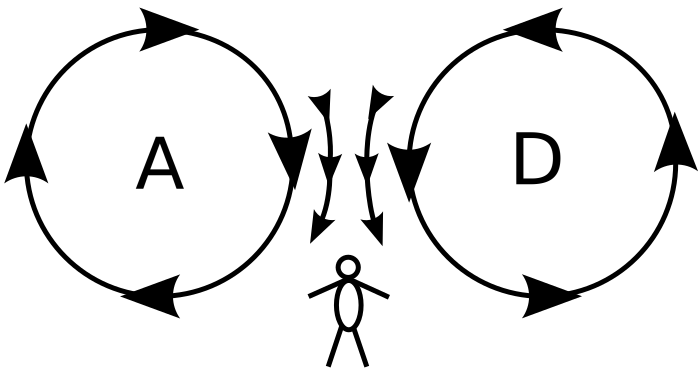
\includegraphics[width=0.4\linewidth]{03-Meteo/img/buysBallot.pdf}
			\legende{Illustration de la loi de Buys-Ballot}{img:buysBallot}
		\end{figure}	
		
		\astuce{Pour s'en souvenir, dans l'hémisphère nord (le notre) : les A : f\textbf{a}ce au vent, \textbf{a}nticyclone à g\textbf{a}uche.}
		\input{03-Meteo/05-PhenomenesDangereux.tex}
	\fi
	
	\chapter{Aérodynamique, aérostatique et principes du vol}
	\label{aerodynamique}
	    Dans ce chapitre, nous allons aborder l'un des composant majeur de la structure d'un aérodyne, celui qui le fait voler : son aile.

Nous décrirons dans un premier temps ce qu'est une aile et quelles sont ses caractéristiques. Nous étudierons notamment les différents types d'ailes.

Nous verrons ensuite quels sont les grands principes du vol stabilisé, ainsi qu'en montée et en descente.

Enfin, nous étudierons l'aérostatique (le vol des aérostats) et le vol spatial.
		\section{La sustentation et l'aile}

\subsection{L'aile : description}

\subsubsection{Description générale}
Toute aile est composée de plusieurs parties distinctes :
\begin{itemize}
	\item L'\gls{intrados} est la partie inférieure de l'aile. Lorsque l'aile se déplace dans une masse d'air, l'intrados est le siège d'une surpression.
	\item L'\gls{extrados} est la partie supérieure de l'aile. Lorsque l'aile se déplace dans une masse d'air, l'extrados est le siège d'une dépression (l'aile est aspirée vers le haut).
	\item Le \gls{bord d'attaque} \anglais{leading edge} est le point le plus en avant d'un profil d'aile. C'est à ce point que l'air entrera en contact en premier avec l'aile. Il s'agit généralement d'une surface  courbe.
	\item Le \gls{bord de fuite} \anglais{trailing edge} est le point le plus en arrière d'un profil d'aile.  Il s'agit généralement d'une surface pointue.
\end{itemize}

	\begin{figure}[H]
  	\centering
    \includegraphics[width=0.8\textwidth]{04-Aerodynamique/img/profilAile}
  	\legende{Profil d'une aile}{img:profilAile}
	\end{figure}	
	
	\astuce{Pour se souvenir ou sont situés l'intrados et l'extrados : que l'avion vol à plat, l'extrados fait face à l'extérieur de la planète, l'intrados regarde vers l'intérieur de la planète.} 	


		\section{Étude du vol stabilisé}
	\subsection{Vol plané}
	
	\subsection{Vol stabilisé}
		\section{L'aérostation}
	\subsection{Principe généraux}
		\section{Le vol spatial}
	\subsection{Principe généraux}
	
	\ifdefined\activerrelease 
	\else
	\chapter{Histoire et culture de l'aéronautique et du spatial}
	\label{histoire}
		\section{Du mythe à la réalité}
		\section{Des précurseurs aux pionniers}
		\section{Les enjeux militaires et les évolutions de l'aéronautique et du spatial}
		\section{Les enjeux économiques et les évolutions de l'aéronautique et du spatial}
	\fi
		
	\appendix
	\ifdefined\activerrelease 
	\else
	\chapter{Dossier de vol}	
		\section{Log de navigation}
		\section{Masse et centrage}
		\section{Dossier météo}
			\subsection{TEMSI}
			\subsection{WINTEM}
			\subsection{TAF et METAR}
	\fi
	
	\chapter{Fiches pratiques}
		\section{Tableau des unités usuelles en aviation}	
	
	\begin{longtable}{
	|>{\centering}m{1.8cm}
	|>{\centering}m{2.8cm}
	|c
	|>{\centering}m{3.2cm}
	|c
	|}

 \hline
 Grandeur & Unité aéronautique & Abbrev. &  Valeur exacte & Valeur approchée\\
 \hline
 %\endfirsthead
 Hauteur Altitude & pieds \anglais{feet}\footnote{Le pied est utilisé pour l'altitude en aéronautique partout dans le monde sauf en Russie, qui utilise le mètre. Les vélivoles (planeurs) utilisent également le mètre pour l'altitude} & ft & 1~ft = 0,3048~m & 1~m $\approx$ 3~pieds \\
 \hline
 Vitesse verticale & pieds/minute & ft/min & 1000~ft/min = 5,08~m/s & 1000~ft/min $\approx$ 5~m/s \\
 \hline
 Distance & mille nautique \anglais{nautical mile} & NM & 1~NM = 1852~m & \\
 \hline
 Vitesse & nœud \anglais{knot} & kt & 1~kt~=~1~NM/h 1~kt~=~1,852~km/h & \\
 \hline
 
 \caption{Tableau récapitulatif des unités utilisées en aéronautique}
 \end{longtable}
	
		\begin{center}
	\begin{longtable}{|L{0.5cm}|L{3.5cm}||L{0.5cm}|L{3.5cm}||L{0.5cm}|L{3.5cm}|}
		\hline
			A & Alpha & 				J & Juliett &			S & Sierra \tabularnewline
		\hline
			B & Bravo & 				K & Kilo &				T & Tango \tabularnewline
		\hline
			C & Charlie & 			L & Lima &				U & Uniform \tabularnewline
		\hline
			D & Delta & 				M & Mike &				V & Victor \tabularnewline	
		\hline
			E & Echo & 				N & November &			W & Wiskey \tabularnewline
		\hline
			F & Fox-trot & 			O & Oscar &				X & X-Ray \tabularnewline
		\hline
			G & Golf & 				P & Papa &				Y & Yankee \tabularnewline
		\hline
			H & Hotel & 				Q & Quebec &				Z & Zoulou \tabularnewline
		\hline
			I & India & 				R & Romeo &				0 & Zéro \anglais{zero} \tabularnewline
		\hline
			1 & Unité \anglais{one} & 2 & Deux \anglais{two}   & 3 & Trois \anglais{three} \tabularnewline
		\hline
			4 & Quatre \anglais{four} & 5 & Cinq \anglais{five} &	6 & Six \anglais{six} \tabularnewline
		\hline
			7 & Sept \anglais{sevent} & 	8 & Huit \anglais{eight} & 9 & Neuf \anglais{nine\footnote{Prononcé 'niner'}} \tabularnewline
		\hline
	\caption{L'alphabet radio international}
	\end{longtable}
\end{center}
	
	\ifdefined\activerrelease 
	\else
	\chapter{Des questions pour pousser la réflexion !}
		\section{Étude des aéronefs}
		\question{"Le parachute est-il un aéronef ? Pourquoi ?" (en parlant du parachute coupole)}
	\fi
	
	\chapter{Frise chronologique}
		Les évenément présentés ici sont également disponibles de façon visuelle et interactive \href{http://brevet.initiation.aero/friseChronologique.html}{en ligne sur la frise chronologique}\footnote{\url{http://brevet.initiation.aero/friseChronologique.html}}.
		\section{Mythes et précurseurs}

\begin{table}[H]
    \centering
    \begin{tabular}{c l c}
        \begin{minipage}{.075\textwidth}
            \begin{figure}[H]
                \centering
                
\includegraphics[width=1.0\linewidth]{Annexes/friseChronologique/img/Flag_of_Greece.pdf}
                \captionsetup{labelformat=empty}\refDrapeau{Drapeau Greece}{frise:Flag_of_Greece.pdf}
            \end{figure}
        \end{minipage}
    &
        \begin{minipage}{.65\textwidth}
            \textbf{-800} - \textbf{Le mythe d'Icare}
            
            Dans la mythologie grecque, Dédale fabrique des ailes en plumes et en cire pour lui et son fils Icare afin de s'échapper du labyrinthe. Icare, s'approchant trop près du soleil, voit la cire fondre et tombe dans la mer. Ce mythe illustre depuis l'Antiquité le rêve ancestral de l'Homme de voler.
            \begin{figure}[H]
                \legende{Icare et Dédale}{frise:Anthony_van_Dyck_-_Daedalus_and_Icarus_-_Google_Art_Project.jpg}
            \end{figure}
        \end{minipage}
    &
        \begin{minipage}{.275\textwidth}
            \begin{figure}[H]
                \centering
                \includegraphics[width=1.0\linewidth]{Annexes/friseChronologique/img/Anthony_van_Dyck_-_Daedalus_and_Icarus_-_Google_Art_Project.jpg}
            \end{figure}
        \end{minipage}
    \end{tabular}
\end{table}
\begin{table}[H]
    \centering
    \begin{tabular}{c l c}
        \begin{minipage}{.075\textwidth}
            \begin{figure}[H]
                \centering
                
\includegraphics[width=1.0\linewidth]{Annexes/friseChronologique/img/Flag_of_the_People27s_Republic_of_China.pdf}
                \captionsetup{labelformat=empty}\refDrapeau{Drapeau the People27s Republic of China}{frise:Flag_of_the_People27s_Republic_of_China.pdf}
            \end{figure}
        \end{minipage}
    &
        \begin{minipage}{.65\textwidth}
            \textbf{-200} - \textbf{Invention du cerf-volant}
            
            Le cerf-volant est inventé en Chine vers 200 avant J.-C. Il sera utilisé pendant des siècles pour des applications militaires, religieuses et scientifiques. Au XVIIIe siècle, les cerfs-volants serviront aux premières expériences scientifiques sur l'aérodynamique.
            \begin{figure}[H]
                \legende{Cerf-volant moderne}{frise:Chinese_Kite.jpg}
            \end{figure}
        \end{minipage}
    &
        \begin{minipage}{.275\textwidth}
            \begin{figure}[H]
                \centering
                \includegraphics[width=1.0\linewidth]{Annexes/friseChronologique/img/Chinese_Kite.jpg}
            \end{figure}
        \end{minipage}
    \end{tabular}
\end{table}
\begin{table}[H]
    \centering
    \begin{tabular}{c l c}
        \begin{minipage}{.075\textwidth}
            \begin{figure}[H]
                \centering
                
\includegraphics[width=1.0\linewidth]{Annexes/friseChronologique/img/Flag_of_John_the_Baptist.pdf}
                \captionsetup{labelformat=empty}\refDrapeau{Drapeau John the Baptist}{frise:Flag_of_John_the_Baptist.pdf}
            \end{figure}
        \end{minipage}
    &
        \begin{minipage}{.65\textwidth}
            \textbf{1485} - \textbf{Léonard de Vinci, visionnaire du vol}
            
            Léonard de Vinci étudie le vol des oiseaux et conçoit de nombreuses machines volantes dans ses carnets : l'ornithoptère (machine à ailes battantes), le parachute pyramidal, et une vis aérienne (ancêtre de l'hélicoptère). Bien que jamais construites de son vivant, ses études pionnières influenceront les inventeurs futurs.
            \begin{figure}[H]
                \legende{Étude de la vis aérienne de Léonard de Vinci}{frise:Leonardo_helicopter.JPG}
            \end{figure}
        \end{minipage}
    &
        \begin{minipage}{.275\textwidth}
            \begin{figure}[H]
                \centering
                \includegraphics[width=1.0\linewidth]{Annexes/friseChronologique/img/Leonardo_helicopter.JPG}
            \end{figure}
        \end{minipage}
    \end{tabular}
\end{table}
\section{L'aérostation}

\begin{table}[H]
    \centering
    \begin{tabular}{c l c}
        \begin{minipage}{.075\textwidth}
            \begin{figure}[H]
                \centering
                
\includegraphics[width=1.0\linewidth]{Annexes/friseChronologique/img/Flag_of_France.pdf}
                \captionsetup{labelformat=empty}\refDrapeau{Drapeau France}{frise:Flag_of_France.pdf}
            \end{figure}
            
            \centering\mdiBrevet
        \end{minipage}
    &
        \begin{minipage}{.65\textwidth}
            \textbf{1732} - \textbf{Henri Pitot invente le tube de Pitot}
            
            Le tube de Pitot est inventé en 1732 par le physicien Henri Pitot, pour la mesure de la vitesse des bateaux ou des vitesse d'écoulement de l'eau dans les rivière. Le tube de Pitot sera ensuite utilisé en aéronautique dans les dispositifs de mesure de vitesse des aéronefs.
            \begin{figure}[H]
                \legende{Portrait de Henri Pitot}{frise:Henri_de_Pitot.jpg}
            \end{figure}
        \end{minipage}
    &
        \begin{minipage}{.275\textwidth}
            \begin{figure}[H]
                \centering
                \includegraphics[width=1.0\linewidth]{Annexes/friseChronologique/img/Henri_de_Pitot.jpg}
            \end{figure}
        \end{minipage}
    \end{tabular}
\end{table}
\begin{table}[H]
    \centering
    \begin{tabular}{c l c}
        \begin{minipage}{.075\textwidth}
            \begin{figure}[H]
                \centering
                
\includegraphics[width=1.0\linewidth]{Annexes/friseChronologique/img/Flag_of_France.pdf}
                \captionsetup{labelformat=empty}\refDrapeau{Drapeau France}{frise:Flag_of_France.pdf}
            \end{figure}
            
            \centering\mdiAirBalloon
        \end{minipage}
    &
        \begin{minipage}{.65\textwidth}
            \textbf{1783} - \textbf{Premier vol en montgolfière}
            
            Pilâtre de Rosier s'élève dans le ciel grâce à la montgolfière des frères Montgoflier
            \begin{figure}[H]
                \legende{Ascension captive d'une montgolfière (Jean-François Pilâtre de Rozier) dans les jardins de la papèterie Réveillon, le 19 octobre 1783.}{frise:Montgolfiere_1783.jpg}
            \end{figure}
        \end{minipage}
    &
        \begin{minipage}{.275\textwidth}
            \begin{figure}[H]
                \centering
                \includegraphics[width=1.0\linewidth]{Annexes/friseChronologique/img/Montgolfiere_1783.jpg}
            \end{figure}
        \end{minipage}
    \end{tabular}
\end{table}
\begin{table}[H]
    \centering
    \begin{tabular}{c l c}
        \begin{minipage}{.075\textwidth}
            \begin{figure}[H]
                \centering
                
\includegraphics[width=1.0\linewidth]{Annexes/friseChronologique/img/Flag_of_France.pdf}
                \captionsetup{labelformat=empty}\refDrapeau{Drapeau France}{frise:Flag_of_France.pdf}
            \end{figure}
            
            \centering\mdiAirBalloon
        \end{minipage}
    &
        \begin{minipage}{.65\textwidth}
            \textbf{1785} - \textbf{Première traversée de la manche}
            
            Jean-Pierre Blanchard traverse la Manche en ballon
            \begin{figure}[H]
                \legende{Traversée en ballon du Pas-de-Calais par Blanchard et Jefferies (1785)}{frise:Early_flight_02562u_28729.jpg}
            \end{figure}
        \end{minipage}
    &
        \begin{minipage}{.275\textwidth}
            \begin{figure}[H]
                \centering
                \includegraphics[width=1.0\linewidth]{Annexes/friseChronologique/img/Early_flight_02562u_28729.jpg}
            \end{figure}
        \end{minipage}
    \end{tabular}
\end{table}
\begin{table}[H]
    \centering
    \begin{tabular}{c l c}
        \begin{minipage}{.075\textwidth}
            \begin{figure}[H]
                \centering
                
\includegraphics[width=1.0\linewidth]{Annexes/friseChronologique/img/Flag_of_France.pdf}
                \captionsetup{labelformat=empty}\refDrapeau{Drapeau France}{frise:Flag_of_France.pdf}
            \end{figure}
            
            \centering\mdiAirBalloon
            
            \centering\mdiParachute
        \end{minipage}
    &
        \begin{minipage}{.65\textwidth}
            \textbf{1797} - \textbf{Premier saut en parachute}
            
            André-Jacques Garnerin effectue le premier saut en parachute, depuis un ballon
            \begin{figure}[H]
                \legende{N°. 4 – Descente de Jacques Garnerin en parachute (1797)}{frise:Early_flight_02561u_28429.jpg}
            \end{figure}
        \end{minipage}
    &
        \begin{minipage}{.275\textwidth}
            \begin{figure}[H]
                \centering
                \includegraphics[width=1.0\linewidth]{Annexes/friseChronologique/img/Early_flight_02561u_28429.jpg}
            \end{figure}
        \end{minipage}
    \end{tabular}
\end{table}
\begin{table}[H]
    \centering
    \begin{tabular}{c l c}
        \begin{minipage}{.075\textwidth}
            \begin{figure}[H]
                \centering
                
\includegraphics[width=1.0\linewidth]{Annexes/friseChronologique/img/Flag_of_France.pdf}
                \captionsetup{labelformat=empty}\refDrapeau{Drapeau France}{frise:Flag_of_France.pdf}
            \end{figure}
            
            \centering\mdiAirBalloon
        \end{minipage}
    &
        \begin{minipage}{.65\textwidth}
            \textbf{1852} - \textbf{Premier vol en dirigeable}
            
            L'ingénieur français Henri Giffard fit voler le premier dirigeable
        \end{minipage}
    &
        \begin{minipage}{.275\textwidth}
            \begin{figure}[H]
                \centering
                \includegraphics[width=1.0\linewidth]{Annexes/friseChronologique/vide.pdf}
            \end{figure}
        \end{minipage}
    \end{tabular}
\end{table}
\begin{table}[H]
    \centering
    \begin{tabular}{c l c}
        \begin{minipage}{.075\textwidth}
            \begin{figure}[H]
                \centering
                
\includegraphics[width=1.0\linewidth]{Annexes/friseChronologique/img/Flag_of_France.pdf}
                \captionsetup{labelformat=empty}\refDrapeau{Drapeau France}{frise:Flag_of_France.pdf}
            \end{figure}
            
            \centering\mdiAirBalloon
        \end{minipage}
    &
        \begin{minipage}{.65\textwidth}
            \textbf{1858} - \textbf{Nadar réalise la première photographie aérienne}
            
            Felix Tournachon dit "Nadar" devient le premier photographe aérien en réalisant une prise de vue de Paris depuis un ballon.
            \begin{figure}[H]
                \legende{Nadar élevant la Photographie à la hauteur de l'Art., lithographie d'Honoré Daumier parue dans Le Boulevard, le 25 mai 1863}{frise:HonorC3A9_Daumier2C_Nadar_C3A9levant_la_Photographie_C3A0_la_hauteur_de_l27Art2C_18622C_NGA_42966.jpg}
            \end{figure}
        \end{minipage}
    &
        \begin{minipage}{.275\textwidth}
            \begin{figure}[H]
                \centering
                \includegraphics[width=1.0\linewidth]{Annexes/friseChronologique/img/HonorC3A9_Daumier2C_Nadar_C3A9levant_la_Photographie_C3A0_la_hauteur_de_l27Art2C_18622C_NGA_42966.jpg}
            \end{figure}
        \end{minipage}
    \end{tabular}
\end{table}
\section{Les pionniers du plus lourd que l'air}

\begin{table}[H]
    \centering
    \begin{tabular}{c l c}
        \begin{minipage}{.075\textwidth}
            \begin{figure}[H]
                \centering
                \includegraphics[width=1.0\linewidth]{Annexes/friseChronologique/img/Flag_of_France.pdf}
                \captionsetup{labelformat=empty}\refDrapeau{Drapeau France}{frise:Flag_of_France.pdf}
            \end{figure}
        \end{minipage}
    &
        \begin{minipage}{.65\textwidth}
            \textbf{1890} - \textbf{Clément Ader met au point l'Eole}
            
            Clément Ader, ingénieur français, conçoit l'Eole puis les Avions, aérodynes en forme de chauves-souris. Bien que Clément Ader affirma à partir de 1906 que ses aérodynes soient parvnus à réaliser des vols de 300 m, on manque de preuve pour attester ces affirmations. Pour cette raison, on ne retient pas Ader comme ayant été le premier à effectuer un vol contrôlé.
            \begin{figure}[H]
                \legende{L’Avion III de Clément Ader}{frise:Avion_III_Art_et_Metiers.jpg}
            \end{figure}
        \end{minipage}
    &
        \begin{minipage}{.275\textwidth}
            \begin{figure}[H]
                \centering
                \includegraphics[width=1.0\linewidth]{Annexes/friseChronologique/img/Avion_III_Art_et_Metiers.jpg}
            \end{figure}
        \end{minipage}
    \end{tabular}
\end{table}
\begin{table}[H]
    \centering
    \begin{tabular}{c l c}
        \begin{minipage}{.075\textwidth}
            \begin{figure}[H]
                \centering
                \includegraphics[width=1.0\linewidth]{Annexes/friseChronologique/img/Flag_of_Germany.pdf}
                \captionsetup{labelformat=empty}\refDrapeau{Drapeau Germany}{frise:Flag_of_Germany.pdf}
            \end{figure}
        \end{minipage}
    &
        \begin{minipage}{.65\textwidth}
            \textbf{1891} - \textbf{Premier vol en planeur}
            
            L'ingénieur allemand Otto Lilienthal fait voler son planeur, en se lancant depuis une colline
            \begin{figure}[H]
                \legende{L'un des vols d'Otto Lilienthal, ici en 1895}{frise:Otto_Lilienthal_gliding_experiment_ppmsca.02546.jpg}
            \end{figure}
        \end{minipage}
    &
        \begin{minipage}{.275\textwidth}
            \begin{figure}[H]
                \centering
                \includegraphics[width=1.0\linewidth]{Annexes/friseChronologique/img/Otto_Lilienthal_gliding_experiment_ppmsca.02546.jpg}
            \end{figure}
        \end{minipage}
    \end{tabular}
\end{table}
\begin{table}[H]
    \centering
    \begin{tabular}{c l c}
        \begin{minipage}{.075\textwidth}
            \begin{figure}[H]
                \centering
                \includegraphics[width=1.0\linewidth]{Annexes/friseChronologique/img/Flag_of_the_United_States_28DDD-F-416E_specifications29.pdf}
                \captionsetup{labelformat=empty}\refDrapeau{Drapeau the United States 28DDD-F-416E specifications29}{frise:Flag_of_the_United_States_28DDD-F-416E_specifications29.pdf}
            \end{figure}
        \end{minipage}
    &
        \begin{minipage}{.65\textwidth}
            \textbf{1896} - \textbf{Octave Chanute et le vol plané}
            
            L'ingénieur franco-américain Octave Chanute perfectionne les planeurs et effectue des centaines de vols. Ses travaux, notamment sur la structure biplan, influenceront directement les frères Wright. Il joue un rôle crucial dans la diffusion des connaissances aéronautiques.
            \begin{figure}[H]
                \legende{Planeur d'Octave Chanute en 1896}{frise:Chanute-Herring_1896_hang_glider.jpg}
            \end{figure}
        \end{minipage}
    &
        \begin{minipage}{.275\textwidth}
            \begin{figure}[H]
                \centering
                \includegraphics[width=1.0\linewidth]{Annexes/friseChronologique/img/Chanute-Herring_1896_hang_glider.jpg}
            \end{figure}
        \end{minipage}
    \end{tabular}
\end{table}
\begin{table}[H]
    \centering
    \begin{tabular}{c l c}
        \begin{minipage}{.075\textwidth}
            \begin{figure}[H]
                \centering
                \includegraphics[width=1.0\linewidth]{Annexes/friseChronologique/img/Flag_of_France.pdf}
                \captionsetup{labelformat=empty}\refDrapeau{Drapeau France}{frise:Flag_of_France.pdf}
            \end{figure}
        \end{minipage}
    &
        \begin{minipage}{.65\textwidth}
            \textbf{19 octobre 1901} - \textbf{Alberto Santos Dumont contourne la Tour Eiffel en dirigeable}
            
            
            \begin{figure}[H]
                \legende{Internet Archive Book Images}{frise:Santos-Dumont_flight_around_the_Eiffel_Tower.jpg}
            \end{figure}
        \end{minipage}
    &
        \begin{minipage}{.275\textwidth}
            \begin{figure}[H]
                \centering
                \includegraphics[width=1.0\linewidth]{Annexes/friseChronologique/img/Santos-Dumont_flight_around_the_Eiffel_Tower.jpg}
            \end{figure}
        \end{minipage}
    \end{tabular}
\end{table}
\begin{table}[H]
    \centering
    \begin{tabular}{c l c}
        \begin{minipage}{.075\textwidth}
            \begin{figure}[H]
                \centering
                \includegraphics[width=1.0\linewidth]{Annexes/friseChronologique/img/Flag_of_the_United_States_28DDD-F-416E_specifications29.pdf}
                \captionsetup{labelformat=empty}\refDrapeau{Drapeau the United States 28DDD-F-416E specifications29}{frise:Flag_of_the_United_States_28DDD-F-416E_specifications29.pdf}
            \end{figure}
        \end{minipage}
    &
        \begin{minipage}{.65\textwidth}
            \textbf{1903} - \textbf{Premier vol d'un avion}
            
            Les frères Orville et Wilbur Wright font voler leur avion aux Etats-Unis.
Il s'agit du premier vol contrôlé d'un aérodyne motorisé
            \begin{figure}[H]
                \legende{Premier vol motorisé des frères Wright le 17 décembre 1903 sur Flyer.}{frise:Wrightflyer.jpg}
            \end{figure}
        \end{minipage}
    &
        \begin{minipage}{.275\textwidth}
            \begin{figure}[H]
                \centering
                \includegraphics[width=1.0\linewidth]{Annexes/friseChronologique/img/Wrightflyer.jpg}
            \end{figure}
        \end{minipage}
    \end{tabular}
\end{table}
\begin{table}[H]
    \centering
    \begin{tabular}{c l c}
        \begin{minipage}{.075\textwidth}
            \begin{figure}[H]
                \centering
                \includegraphics[width=1.0\linewidth]{Annexes/friseChronologique/img/Flag_of_France.pdf}
                \captionsetup{labelformat=empty}\refDrapeau{Drapeau France}{frise:Flag_of_France.pdf}
            \end{figure}
            
            \centering\mdiBrevet
        \end{minipage}
    &
        \begin{minipage}{.65\textwidth}
            \textbf{22 janvier 1907} - \textbf{Invention du manche à balai}
            
            Robert Esnault-Pelterie dépose le brevet pour le manche à balai, permettant de diriger les aéronefs
            \begin{figure}[H]
                \legende{Portrait de Robert Esnault-Pelterie}{frise:Robert_Esnault-Pelterie_1909.jpg}
            \end{figure}
        \end{minipage}
    &
        \begin{minipage}{.275\textwidth}
            \begin{figure}[H]
                \centering
                \includegraphics[width=1.0\linewidth]{Annexes/friseChronologique/img/Robert_Esnault-Pelterie_1909.jpg}
            \end{figure}
        \end{minipage}
    \end{tabular}
\end{table}
\begin{table}[H]
    \centering
    \begin{tabular}{c l c}
        \begin{minipage}{.075\textwidth}
            \begin{figure}[H]
                \centering
                \includegraphics[width=1.0\linewidth]{Annexes/friseChronologique/img/Flag_of_France.pdf}
                \captionsetup{labelformat=empty}\refDrapeau{Drapeau France}{frise:Flag_of_France.pdf}
            \end{figure}
            
            \centering\mdiFemale
        \end{minipage}
    &
        \begin{minipage}{.65\textwidth}
            \textbf{08 juillet 1908} - \textbf{Thérèse Peltier, première femme à quitter le sol}
            
            Le 8 juillet 1908, Thérèse Peltier devient la premier femme à quitter le sol avec un aéronef, dans un avion piloté par son compagnon Léon Delagrange.

Elle deviendra la première femme à voler seule à bord d'un avion quelque mois plus tard, lors de son lâcher solo.
            \begin{figure}[H]
                \legende{Thérèse Peltier à Issy-les-Moulineaux le 17 September 1908}{frise:ThC3A9rC3A8se_Peltier_1908.jpg}
            \end{figure}
        \end{minipage}
    &
        \begin{minipage}{.275\textwidth}
            \begin{figure}[H]
                \centering
                \includegraphics[width=1.0\linewidth]{Annexes/friseChronologique/img/ThC3A9rC3A8se_Peltier_1908.jpg}
            \end{figure}
        \end{minipage}
    \end{tabular}
\end{table}
\begin{table}[H]
    \centering
    \begin{tabular}{c l c}
        \begin{minipage}{.075\textwidth}
            \begin{figure}[H]
                \centering
                \includegraphics[width=1.0\linewidth]{Annexes/friseChronologique/img/Flag_of_France.pdf}
                \captionsetup{labelformat=empty}\refDrapeau{Drapeau France}{frise:Flag_of_France.pdf}
            \end{figure}
        \end{minipage}
    &
        \begin{minipage}{.65\textwidth}
            \textbf{25 juillet 1909} - \textbf{Louis Blériot traverse la manche}
            
            "L'Angleterre n'est plus une île !" Le 25 juillet 1909, Louis Blériot relie Calais à Douvres à bord de son  Blériot XI.
            \begin{figure}[H]
                \legende{Blériot aux commandes de l'appareil de la traversée à la fête de Port-Aviation, le 4 juillet 1909.}{frise:Btv1b8433368f-p044_BlC3A9riot_C3A0_la_fC3AAte_de_Port-Aviation2C_dimanche_4_juillet_1909.jpg}
            \end{figure}
        \end{minipage}
    &
        \begin{minipage}{.275\textwidth}
            \begin{figure}[H]
                \centering
                \includegraphics[width=1.0\linewidth]{Annexes/friseChronologique/img/Btv1b8433368f-p044_BlC3A9riot_C3A0_la_fC3AAte_de_Port-Aviation2C_dimanche_4_juillet_1909.jpg}
            \end{figure}
        \end{minipage}
    \end{tabular}
\end{table}
\begin{table}[H]
    \centering
    \begin{tabular}{c l c}
        \begin{minipage}{.075\textwidth}
            \begin{figure}[H]
                \centering
                \includegraphics[width=1.0\linewidth]{Annexes/friseChronologique/img/Flag_of_France.pdf}
                \captionsetup{labelformat=empty}\refDrapeau{Drapeau France}{frise:Flag_of_France.pdf}
            \end{figure}
        \end{minipage}
    &
        \begin{minipage}{.65\textwidth}
            \textbf{07 octobre 1909} - \textbf{Louis Blériot obtient le premier brevet de pilote}
            
            Le brevet de pilote n°1 est délivré à Louis Blériot

Le 7 octobre 1909, l'Aéro-Club de France décide de décerner un brevet de pilote à seize pionniers de l'aviation. Personne n’osant faire passer un examen à ces pionniers, un comité prit la liste des pilotes et les classa par ordre alphabétique. Son nom commençant par un B, Louis Blériot se voit attribuer le brevet de pilote numéro 1. L’instauration du brevet de pilote intervient le 1er janvier 1910.
            \begin{figure}[H]
                \legende{Avant de délivrer des brevets de pilotes d'avion, l'Aéroclub de France délivrait également des brevets aux pilotes de ballons. Brevet de pilote aéronaute décerné par l'Aéro-Club de France à Paul Tissandier (1904).}{frise:Brevet_de_pilote_aC3A9ronaute_1904.jpg}
            \end{figure}
        \end{minipage}
    &
        \begin{minipage}{.275\textwidth}
            \begin{figure}[H]
                \centering
                \includegraphics[width=1.0\linewidth]{Annexes/friseChronologique/img/Brevet_de_pilote_aC3A9ronaute_1904.jpg}
            \end{figure}
        \end{minipage}
    \end{tabular}
\end{table}
\begin{table}[H]
    \centering
    \begin{tabular}{c l c}
        \begin{minipage}{.075\textwidth}
            \begin{figure}[H]
                \centering
                \includegraphics[width=1.0\linewidth]{Annexes/friseChronologique/img/Flag_of_France.pdf}
                \captionsetup{labelformat=empty}\refDrapeau{Drapeau France}{frise:Flag_of_France.pdf}
            \end{figure}
            
            \centering\mdiFemale
        \end{minipage}
    &
        \begin{minipage}{.65\textwidth}
            \textbf{08 mars 1910} - \textbf{Élisa Deroche, première femme brevetée pilote}
            
            Élisa Deroche s'interesse à l'aviation depuis l'année 1906.
Fin 1909, elle effectue son premier vol solo, et son brevet (le n°36) lui sera délivré quelques mois plus tard, le 8 mars 1910.

La semaine internationale des femmes de l'air marque désormais chaque année cette date historique, puisque cette semaine est positionnée sur la semaine du 8 mars. 

            \begin{figure}[H]
                \legende{Elise Deroche aux commandes d'un biplan Voisin.}{frise:Les_Maitres_de_l27aviation._Mme._la_Baronne_de_Laroche2C_aviatrice2C_au_poste_de_direction_d27un_biplan_Voisin._cph.3c07402.jpg}
            \end{figure}
        \end{minipage}
    &
        \begin{minipage}{.275\textwidth}
            \begin{figure}[H]
                \centering
                \includegraphics[width=1.0\linewidth]{Annexes/friseChronologique/img/Les_Maitres_de_l27aviation._Mme._la_Baronne_de_Laroche2C_aviatrice2C_au_poste_de_direction_d27un_biplan_Voisin._cph.3c07402.jpg}
            \end{figure}
        \end{minipage}
    \end{tabular}
\end{table}
\begin{table}[H]
    \centering
    \begin{tabular}{c l c}
        \begin{minipage}{.075\textwidth}
            \begin{figure}[H]
                \centering
                \includegraphics[width=1.0\linewidth]{Annexes/friseChronologique/img/Flag_of_France.pdf}
                \captionsetup{labelformat=empty}\refDrapeau{Drapeau France}{frise:Flag_of_France.pdf}
            \end{figure}
        \end{minipage}
    &
        \begin{minipage}{.65\textwidth}
            \textbf{28 mars 1910} - \textbf{Premier vol d'un hydravion}
            
            L'ingénieur français Henri Fabre devient le premier à décoller d'un plan d'eau avec un aéronef qui dispose de son propre moyen de propulsion. Cette date marque l'entrée dans l'ère de l'hydraviation qui aura son âge d'or sur la période de l'entre 2 guerres.
            \begin{figure}[H]
                \legende{Hydroplane d'Henri Fabre}{frise:Hydroplane_28de_Henri29_Fabre_28Monaco2C_concours_de_canots_automobiles2C_2_-17_avril29_1911_-_btv1b53240713d.jpg}
            \end{figure}
        \end{minipage}
    &
        \begin{minipage}{.275\textwidth}
            \begin{figure}[H]
                \centering
                \includegraphics[width=1.0\linewidth]{Annexes/friseChronologique/img/Hydroplane_28de_Henri29_Fabre_28Monaco2C_concours_de_canots_automobiles2C_2_-17_avril29_1911_-_btv1b53240713d.jpg}
            \end{figure}
        \end{minipage}
    \end{tabular}
\end{table}
\begin{table}[H]
    \centering
    \begin{tabular}{c l c}
        \begin{minipage}{.075\textwidth}
            \begin{figure}[H]
                \centering
                \includegraphics[width=1.0\linewidth]{Annexes/friseChronologique/img/Flag_of_France.pdf}
                \captionsetup{labelformat=empty}\refDrapeau{Drapeau France}{frise:Flag_of_France.pdf}
            \end{figure}
            
            \centering\mdiBrevet
        \end{minipage}
    &
        \begin{minipage}{.65\textwidth}
            \textbf{1911} - \textbf{Raoul Badin invente l'anémomètre}
            
            L'inventeur français invente un dispositif permettant la mesure de la vitesse de l'air dans lequel évolue un aéronef. L'anémomère est parfois appelé "badin" du nom de cet inventeur
            \begin{figure}[H]
                \legende{Illustration d'un anémomètre moderne}{frise:Airspeed_indicator.pdf}
            \end{figure}
        \end{minipage}
    &
        \begin{minipage}{.275\textwidth}
            \begin{figure}[H]
                \centering
                \includegraphics[width=1.0\linewidth]{Annexes/friseChronologique/img/Airspeed_indicator.pdf}
            \end{figure}
        \end{minipage}
    \end{tabular}
\end{table}
\begin{table}[H]
    \centering
    \begin{tabular}{c l c}
        \begin{minipage}{.075\textwidth}
            \begin{figure}[H]
                \centering
                \includegraphics[width=1.0\linewidth]{Annexes/friseChronologique/img/Flag_of_Italy_281861E28093194629.pdf}
                \captionsetup{labelformat=empty}\refDrapeau{Drapeau Italy 281861E28093194629}{frise:Flag_of_Italy_281861E28093194629.pdf}
            \end{figure}
            
            \centering\mdiMilitaire
        \end{minipage}
    &
        \begin{minipage}{.65\textwidth}
            \textbf{23 novembre 1911} - \textbf{Premier usage d'avions au combat}
            
            Les Italiens sont les premiers à utiliser des avions au combat à l'occasion de la guerre de Libye.

Les Italiens utilisent des avions Blériot XI, Nieuport, Farman et Etrich Taube
            \begin{figure}[H]
                \legende{Avion italien lors d'un attaque en Libye}{frise:Italian_Nieuport_IV_attacking_Ottoman_forces_in_Libya_1911_or_1912.jpg}
            \end{figure}
        \end{minipage}
    &
        \begin{minipage}{.275\textwidth}
            \begin{figure}[H]
                \centering
                \includegraphics[width=1.0\linewidth]{Annexes/friseChronologique/img/Italian_Nieuport_IV_attacking_Ottoman_forces_in_Libya_1911_or_1912.jpg}
            \end{figure}
        \end{minipage}
    \end{tabular}
\end{table}
\begin{table}[H]
    \centering
    \begin{tabular}{c l c}
        \begin{minipage}{.075\textwidth}
            \begin{figure}[H]
                \centering
                \includegraphics[width=1.0\linewidth]{Annexes/friseChronologique/img/Flag_of_France.pdf}
                \captionsetup{labelformat=empty}\refDrapeau{Drapeau France}{frise:Flag_of_France.pdf}
            \end{figure}
        \end{minipage}
    &
        \begin{minipage}{.65\textwidth}
            \textbf{21 septembre 1913} - \textbf{Adolphe Pégoud : premier looping}
            
            Le 19 août 1913, Adolphe Pegoud est le premier pilote de l'histoire à utiliser un parachute pour abandonner un avion en perdition.

L'histoire raconte que l'avion qu'il venait de quitter aurait alors effecuté un looping. C'est de cet événément qu'Adolphe Pegoud aurait tiré l'idée de réaliser un looping à bord de son avion, chose qu'il réalise le 21 septembre.
            \begin{figure}[H]
                \legende{Carte postale allemande illustrant le looping d'Adolphe Pegoud.}{frise:Adolphe_PC3A9goud_Looping.jpg}
            \end{figure}
        \end{minipage}
    &
        \begin{minipage}{.275\textwidth}
            \begin{figure}[H]
                \centering
                \includegraphics[width=1.0\linewidth]{Annexes/friseChronologique/img/Adolphe_PC3A9goud_Looping.jpg}
            \end{figure}
        \end{minipage}
    \end{tabular}
\end{table}
\section{La première guerre mondiale}

\begin{table}[H]
    \centering
    \begin{tabular}{c l c}
        \begin{minipage}{.075\textwidth}
            \begin{figure}[H]
                \centering
                \includegraphics[width=1.0\linewidth]{Annexes/friseChronologique/img/Flag_of_France.pdf}
                \captionsetup{labelformat=empty}\refDrapeau{Drapeau France}{frise:Flag_of_France.pdf}
            \end{figure}
        \end{minipage}
    &
        \begin{minipage}{.65\textwidth}
            \textbf{1914} - \textbf{René Fonck, as des as}
            
            René Fonck est le pilote français ayant le plus grand nombre de victoires aériennes (75). Il est surnomé "l'as des as"
            \begin{figure}[H]
                \legende{Portrait de René Fonck}{frise:RenC3A9_Fonck_02.jpg}
            \end{figure}
        \end{minipage}
    &
        \begin{minipage}{.275\textwidth}
            \begin{figure}[H]
                \centering
                \includegraphics[width=1.0\linewidth]{Annexes/friseChronologique/img/RenC3A9_Fonck_02.jpg}
            \end{figure}
        \end{minipage}
    \end{tabular}
\end{table}
\begin{table}[H]
    \centering
    \begin{tabular}{c l c}
        \begin{minipage}{.075\textwidth}
            \begin{figure}[H]
                \centering
                \includegraphics[width=1.0\linewidth]{Annexes/friseChronologique/img/Flag_of_Germany_281867E28093191829.pdf}
                \captionsetup{labelformat=empty}\refDrapeau{Drapeau Germany 281867E28093191829}{frise:Flag_of_Germany_281867E28093191829.pdf}
            \end{figure}
        \end{minipage}
    &
        \begin{minipage}{.65\textwidth}
            \textbf{1914} - \textbf{Manfred von Richtoffen, as de la première guerre mondiale}
            
            Manfred von Richtoffen, pilote allemand, dispose du plus grand nombre de victoires confirmées (80) lors du premier conflit mondial.

Il est connu sous le nom du Baron rouge
            \begin{figure}[H]
                \legende{Le Baron Rouge, Manfred von Richtoffen}{frise:Manfred_von_Richthofen.jpg}
            \end{figure}
        \end{minipage}
    &
        \begin{minipage}{.275\textwidth}
            \begin{figure}[H]
                \centering
                \includegraphics[width=1.0\linewidth]{Annexes/friseChronologique/img/Manfred_von_Richthofen.jpg}
            \end{figure}
        \end{minipage}
    \end{tabular}
\end{table}
\begin{table}[H]
    \centering
    \begin{tabular}{c l c}
        \begin{minipage}{.075\textwidth}
            \begin{figure}[H]
                \centering
                \includegraphics[width=1.0\linewidth]{Annexes/friseChronologique/img/Flag_of_Germany_281867E28093191829.pdf}
                \captionsetup{labelformat=empty}\refDrapeau{Drapeau Germany 281867E28093191829}{frise:Flag_of_Germany_281867E28093191829.pdf}
            \end{figure}
        \end{minipage}
    &
        \begin{minipage}{.65\textwidth}
            \textbf{12 décembre 1915} - \textbf{Premier vol du Junker J1, premier avion entièrement métallique}
            
            
            \begin{figure}[H]
                \legende{Junker J1}{frise:Junkers_J_1_at_DC3B6beritz_1915.jpg}
            \end{figure}
        \end{minipage}
    &
        \begin{minipage}{.275\textwidth}
            \begin{figure}[H]
                \centering
                \includegraphics[width=1.0\linewidth]{Annexes/friseChronologique/img/Junkers_J_1_at_DC3B6beritz_1915.jpg}
            \end{figure}
        \end{minipage}
    \end{tabular}
\end{table}
\begin{table}[H]
    \centering
    \begin{tabular}{c l c}
        \begin{minipage}{.075\textwidth}
            \begin{figure}[H]
                \centering
                \includegraphics[width=1.0\linewidth]{Annexes/friseChronologique/img/Flag_of_France.pdf}
                \captionsetup{labelformat=empty}\refDrapeau{Drapeau France}{frise:Flag_of_France.pdf}
            \end{figure}
        \end{minipage}
    &
        \begin{minipage}{.65\textwidth}
            \textbf{01 février 1916} - \textbf{Marcel Bloch concoit l'hélice Éclair}
            
            Marcel Dassault (qui s'appelait alors Marcel Bloch) dessine l'hélice Éclair. Cette hélice à marqué l'histoire car elle est très performante. Elle sera produite à plus de 4000 exemplaire et montée sur 10 des 20 avions les plus perfomants de l'armée française de cette époque.
            \begin{figure}[H]
                \legende{Le SPAD VII de Georges Guynemer, équipé de l'hélice Eclair}{frise:Georges_Guynemer27s_SPAD_VII2C_Musee_de_l27Air_et_de_l27Espace2C_Le_Bourget2C_Paris._28812284872329.jpg}
            \end{figure}
        \end{minipage}
    &
        \begin{minipage}{.275\textwidth}
            \begin{figure}[H]
                \centering
                \includegraphics[width=1.0\linewidth]{Annexes/friseChronologique/img/Georges_Guynemer27s_SPAD_VII2C_Musee_de_l27Air_et_de_l27Espace2C_Le_Bourget2C_Paris._28812284872329.jpg}
            \end{figure}
        \end{minipage}
    \end{tabular}
\end{table}
\section{L'entre 2 guerres}

\begin{table}[H]
    \centering
    \begin{tabular}{c l c}
        \begin{minipage}{.075\textwidth}
            \begin{figure}[H]
                \centering
                \includegraphics[width=1.0\linewidth]{Annexes/friseChronologique/img/Flag_of_France.pdf}
                \captionsetup{labelformat=empty}\refDrapeau{Drapeau France}{frise:Flag_of_France.pdf}
            \end{figure}
        \end{minipage}
    &
        \begin{minipage}{.65\textwidth}
            \textbf{25 décembre 1918} - \textbf{Georges Latécoère lance l'Aéropostale}
            
            L'Aéropostale est le transport de courrier et frets (colis) par voie aérienne.

Le 25 décembre 1918, il ouvre la ligne entre Toulouse et Barcelone.

Dès 1919, la ligne est étendue jusqu'à Casablanca. Elle sera par la suite prolongée jusqu'à Dakar puis l'Amérique du Sud via Rio au Brésil, puis jusqu'à Buenos-Aires et Santiago du Chili
            \begin{figure}[H]
                \legende{Carte illustrant les lignes de l'aéropostale entre la France et l'Amérique du Sud, en 1930.}{frise:AC3A9ropostale._AmC3A9rique_du_Sud._Maroc_-_AlgC3A9rie_-_Afrique_Occidentale_FranC3A7aise_-_affiche_-_btv1b10104627j.jpg}
            \end{figure}
        \end{minipage}
    &
        \begin{minipage}{.275\textwidth}
            \begin{figure}[H]
                \centering
                \includegraphics[width=1.0\linewidth]{Annexes/friseChronologique/img/AC3A9ropostale._AmC3A9rique_du_Sud._Maroc_-_AlgC3A9rie_-_Afrique_Occidentale_FranC3A7aise_-_affiche_-_btv1b10104627j.jpg}
            \end{figure}
        \end{minipage}
    \end{tabular}
\end{table}
\begin{table}[H]
    \centering
    \begin{tabular}{c l c}
        \begin{minipage}{.075\textwidth}
            \begin{figure}[H]
                \centering
                \includegraphics[width=1.0\linewidth]{Annexes/friseChronologique/img/Flag_of_France.pdf}
                \captionsetup{labelformat=empty}\refDrapeau{Drapeau France}{frise:Flag_of_France.pdf}
            \end{figure}
            
            \centering\mdiFemale
        \end{minipage}
    &
        \begin{minipage}{.65\textwidth}
            \textbf{01 avril 1921} - \textbf{Adrienne Bolland, première femme à traverser la Cordillière des Andes}
            
            Adrienne Bolland traverse la Cordillière en Caudron G3 en 4h15
            \begin{figure}[H]
                \legende{Adrienne Bolland faisant la couverture du magazine argentin El Gráfico le 19 mars 1921}{frise:Adrienne_Bolland_-_El_GrC3A1fico_91.jpg}
            \end{figure}
        \end{minipage}
    &
        \begin{minipage}{.275\textwidth}
            \begin{figure}[H]
                \centering
                \includegraphics[width=1.0\linewidth]{Annexes/friseChronologique/img/Adrienne_Bolland_-_El_GrC3A1fico_91.jpg}
            \end{figure}
        \end{minipage}
    \end{tabular}
\end{table}
\begin{table}[H]
    \centering
    \begin{tabular}{c l c}
        \begin{minipage}{.075\textwidth}
            \begin{figure}[H]
                \centering
                \includegraphics[width=1.0\linewidth]{Annexes/friseChronologique/img/Flag_of_Spain.pdf}
                \captionsetup{labelformat=empty}\refDrapeau{Drapeau Spain}{frise:Flag_of_Spain.pdf}
            \end{figure}
        \end{minipage}
    &
        \begin{minipage}{.65\textwidth}
            \textbf{1923} - \textbf{Premier vol d'un autogire}
            
            Juan de la Cierva effectue le premier vol d'un autogire
            \begin{figure}[H]
                \legende{L'autogire C-6 de Juan de la Cierva (1925)}{frise:Autogyro_at_Farnborough2C_1925_28Our_Generation2C_193829.jpg}
            \end{figure}
        \end{minipage}
    &
        \begin{minipage}{.275\textwidth}
            \begin{figure}[H]
                \centering
                \includegraphics[width=1.0\linewidth]{Annexes/friseChronologique/img/Autogyro_at_Farnborough2C_1925_28Our_Generation2C_193829.jpg}
            \end{figure}
        \end{minipage}
    \end{tabular}
\end{table}
\begin{table}[H]
    \centering
    \begin{tabular}{c l c}
        \begin{minipage}{.075\textwidth}
            \begin{figure}[H]
                \centering
                \includegraphics[width=1.0\linewidth]{Annexes/friseChronologique/img/Flag_of_the_United_States_28DDD-F-416E_specifications29.pdf}
                \captionsetup{labelformat=empty}\refDrapeau{Drapeau the United States 28DDD-F-416E specifications29}{frise:Flag_of_the_United_States_28DDD-F-416E_specifications29.pdf}
            \end{figure}
        \end{minipage}
    &
        \begin{minipage}{.65\textwidth}
            \textbf{20 mai 1927} - \textbf{Charles Lindbergh réalise le premier vol transaltantique }
            
            Charles Lindbergh réalise le premier vol transaltantique entre New-York et Paris, à bord de son avion,  le Spirit of Saint-Louis
            \begin{figure}[H]
                \legende{}{frise:Col_Charles_Lindbergh2C_original2C_hec.21329.jpg}
            \end{figure}
        \end{minipage}
    &
        \begin{minipage}{.275\textwidth}
            \begin{figure}[H]
                \centering
                \includegraphics[width=1.0\linewidth]{Annexes/friseChronologique/img/Col_Charles_Lindbergh2C_original2C_hec.21329.jpg}
            \end{figure}
        \end{minipage}
    \end{tabular}
\end{table}
\begin{table}[H]
    \centering
    \begin{tabular}{c l c}
        \begin{minipage}{.075\textwidth}
            \begin{figure}[H]
                \centering
                \includegraphics[width=1.0\linewidth]{Annexes/friseChronologique/img/Flag_of_France.pdf}
                \captionsetup{labelformat=empty}\refDrapeau{Drapeau France}{frise:Flag_of_France.pdf}
            \end{figure}
            
            \centering\mdiFemale
            
            \centering\faTrophy
        \end{minipage}
    &
        \begin{minipage}{.65\textwidth}
            \textbf{13 juillet 1928} - \textbf{Maryse Bastié, première recordwomen de distance}
            
            
            \begin{figure}[H]
                \legende{L'aviatrice française Maryse Bastié à ses débuts.}{frise:Maryse_bastie.jpg}
            \end{figure}
        \end{minipage}
    &
        \begin{minipage}{.275\textwidth}
            \begin{figure}[H]
                \centering
                \includegraphics[width=1.0\linewidth]{Annexes/friseChronologique/img/Maryse_bastie.jpg}
            \end{figure}
        \end{minipage}
    \end{tabular}
\end{table}
\begin{table}[H]
    \centering
    \begin{tabular}{c l c}
        \begin{minipage}{.075\textwidth}
            \begin{figure}[H]
                \centering
                \includegraphics[width=1.0\linewidth]{Annexes/friseChronologique/img/Flag_of_the_United_States_28DDD-F-416E_specifications29.pdf}
                \captionsetup{labelformat=empty}\refDrapeau{Drapeau the United States 28DDD-F-416E specifications29}{frise:Flag_of_the_United_States_28DDD-F-416E_specifications29.pdf}
            \end{figure}
            
            \centering\mdiFemale
        \end{minipage}
    &
        \begin{minipage}{.65\textwidth}
            \textbf{20 mai 1932} - \textbf{Amelia Earhart traverse l'Atlantique en solitaire}
            
            En 1928, Amelia Earhart traverse l'Atlantique avec Wilmer Stultz et Louis Gordon. Elle devient ainsi la première femme à effectuer une transatlantique en avion.

Le 20 mai 1932, elle réitère la traversée, mais cette fois ci, seule. Elle effectue en une quinzaine d'heures sur son Lockheed Vega la traversée entre entre le Canada et l'Irlande du Nord.
            \begin{figure}[H]
                \legende{Amelia Earhart en 1935}{frise:Amelia_Earhart_1935.jpg}
            \end{figure}
        \end{minipage}
    &
        \begin{minipage}{.275\textwidth}
            \begin{figure}[H]
                \centering
                \includegraphics[width=1.0\linewidth]{Annexes/friseChronologique/img/Amelia_Earhart_1935.jpg}
            \end{figure}
        \end{minipage}
    \end{tabular}
\end{table}
\begin{table}[H]
    \centering
    \begin{tabular}{c l c}
        \begin{minipage}{.075\textwidth}
            \begin{figure}[H]
                \centering
                \includegraphics[width=1.0\linewidth]{Annexes/friseChronologique/img/Flag_of_France.pdf}
                \captionsetup{labelformat=empty}\refDrapeau{Drapeau France}{frise:Flag_of_France.pdf}
            \end{figure}
        \end{minipage}
    &
        \begin{minipage}{.65\textwidth}
            \textbf{1933} - \textbf{Création de la compagnie Air France}
            
            
            \begin{figure}[H]
                \legende{Un Lockheed Super Constellation d'Air France à Heathrow en 1955}{frise:Lockheed_L1049_F-BGNG_Air_France_LAP_08.04.55_edited-2.jpg}
            \end{figure}
        \end{minipage}
    &
        \begin{minipage}{.275\textwidth}
            \begin{figure}[H]
                \centering
                \includegraphics[width=1.0\linewidth]{Annexes/friseChronologique/img/Lockheed_L1049_F-BGNG_Air_France_LAP_08.04.55_edited-2.jpg}
            \end{figure}
        \end{minipage}
    \end{tabular}
\end{table}
\begin{table}[H]
    \centering
    \begin{tabular}{c l c}
        \begin{minipage}{.075\textwidth}
            \begin{figure}[H]
                \centering
                \includegraphics[width=1.0\linewidth]{Annexes/friseChronologique/img/Flag_of_the_United_Kingdom_283-529.pdf}
                \captionsetup{labelformat=empty}\refDrapeau{Drapeau the United Kingdom 283-529}{frise:Flag_of_the_United_Kingdom_283-529.pdf}
            \end{figure}
            
            \centering\mdiBrevet
        \end{minipage}
    &
        \begin{minipage}{.65\textwidth}
            \textbf{1935} - \textbf{Robert Watson-Watt invente le radar}
            
            Le britannique Robert Watson-Watt dépose un brevet pour le radar, qui permet de détecter à distance des objets, et notamment des avions. Durant la seconde guerre mondiale, cett invention donnera un avantage décisif aux britanniques durant la bataille d'Angleterre (1940)
            \begin{figure}[H]
                \legende{Composant d'un radar conçu par Robet Watson-Watt}{frise:Watson_Radar.jpg}
            \end{figure}
        \end{minipage}
    &
        \begin{minipage}{.275\textwidth}
            \begin{figure}[H]
                \centering
                \includegraphics[width=1.0\linewidth]{Annexes/friseChronologique/img/Watson_Radar.jpg}
            \end{figure}
        \end{minipage}
    \end{tabular}
\end{table}
\begin{table}[H]
    \centering
    \begin{tabular}{c l c}
        \begin{minipage}{.075\textwidth}
            \begin{figure}[H]
                \centering
                \includegraphics[width=1.0\linewidth]{Annexes/friseChronologique/img/Flag_of_Germany.pdf}
                \captionsetup{labelformat=empty}\refDrapeau{Drapeau Germany}{frise:Flag_of_Germany.pdf}
            \end{figure}
        \end{minipage}
    &
        \begin{minipage}{.65\textwidth}
            \textbf{1936} - \textbf{Premier vol d'un hélicoptère}
            
            Le Focke-Wulf Fw 61 est le premier hélicoptère ayant effecuté un vol totalement contrôlé
            \begin{figure}[H]
                \legende{Le Focke-Wulf Fw 61 en vol}{frise:Fw_61_V.JPG}
            \end{figure}
        \end{minipage}
    &
        \begin{minipage}{.275\textwidth}
            \begin{figure}[H]
                \centering
                \includegraphics[width=1.0\linewidth]{Annexes/friseChronologique/img/Fw_61_V.JPG}
            \end{figure}
        \end{minipage}
    \end{tabular}
\end{table}
\begin{table}[H]
    \centering
    \begin{tabular}{c l c}
        \begin{minipage}{.075\textwidth}
            \begin{figure}[H]
                \centering
                \includegraphics[width=1.0\linewidth]{Annexes/friseChronologique/img/Flag_of_the_United_Kingdom_283-529.pdf}
                \captionsetup{labelformat=empty}\refDrapeau{Drapeau the United Kingdom 283-529}{frise:Flag_of_the_United_Kingdom_283-529.pdf}
            \end{figure}
        \end{minipage}
    &
        \begin{minipage}{.65\textwidth}
            \textbf{05 mars 1936} - \textbf{Premier vol du Spitfire}
            
            Le Supermarine Spitfire est un chasseur à hélice. Il sera considéré comme le meilleur avion de la seconde guerre mondiale.
            \begin{figure}[H]
                \legende{Un Spitfire}{frise:Ray_Flying_Legends_2005-1.jpg}
            \end{figure}
        \end{minipage}
    &
        \begin{minipage}{.275\textwidth}
            \begin{figure}[H]
                \centering
                \includegraphics[width=1.0\linewidth]{Annexes/friseChronologique/img/Ray_Flying_Legends_2005-1.jpg}
            \end{figure}
        \end{minipage}
    \end{tabular}
\end{table}
\section{La seconde guerre mondiale}

\begin{table}[H]
    \centering
    \begin{tabular}{c l c}
        \begin{minipage}{.075\textwidth}
            \begin{figure}[H]
                \centering
                \includegraphics[width=1.0\linewidth]{Annexes/friseChronologique/img/Flag_of_Germany_281935E28093194529.pdf}
                \captionsetup{labelformat=empty}\refDrapeau{Drapeau Germany 281935E28093194529}{frise:Flag_of_Germany_281935E28093194529.pdf}
            \end{figure}
            
            \centering\mdiMilitaire
        \end{minipage}
    &
        \begin{minipage}{.65\textwidth}
            \textbf{18 juillet 1942} - \textbf{Le Messerschmitt Me 262, premier chasseur à réaction}
            
            Premier chasseur à réaction de l'Histoire, sa mise au point fut cependant longue et son entrée en service dans la Luftwaffe (armée de l'air allemande) en avril 1944 (donc à la fin de la guerre) impliquera que cet avion aura un rôle mineur dans le second conflit mondial.
            \begin{figure}[H]
                \legende{Un Messerschmitt Me 262}{frise:Messerschmitt_Me_262A_at_the_National_Museum_of_the_USAF.jpg}
            \end{figure}
        \end{minipage}
    &
        \begin{minipage}{.275\textwidth}
            \begin{figure}[H]
                \centering
                \includegraphics[width=1.0\linewidth]{Annexes/friseChronologique/img/Messerschmitt_Me_262A_at_the_National_Museum_of_the_USAF.jpg}
            \end{figure}
        \end{minipage}
    \end{tabular}
\end{table}
\begin{table}[H]
    \centering
    \begin{tabular}{c l c}
        \begin{minipage}{.075\textwidth}
            \begin{figure}[H]
                \centering
                \includegraphics[width=1.0\linewidth]{Annexes/friseChronologique/img/Flag_of_Germany_281935E28093194529.pdf}
                \captionsetup{labelformat=empty}\refDrapeau{Drapeau Germany 281935E28093194529}{frise:Flag_of_Germany_281935E28093194529.pdf}
            \end{figure}
            
            \centering\mdiRocket
            
            \centering\mdiMilitaire
        \end{minipage}
    &
        \begin{minipage}{.65\textwidth}
            \textbf{03 octobre 1942} - \textbf{Premier vol d'un missile balistique V2}
            
            L'Allemagne nazie réalise le premier lancement réussi d'un missile V2. Ce type de missile, mis au point sous l'égide de Wener Von Braun, sont des fusées utilisées pour bombarder principalement le Royaume-Unis et la Belgique.
            \begin{figure}[H]
                \legende{Réplique de missile V2, Usedom, Allemagne}{frise:La2-v2.jpg}
            \end{figure}
        \end{minipage}
    &
        \begin{minipage}{.275\textwidth}
            \begin{figure}[H]
                \centering
                \includegraphics[width=1.0\linewidth]{Annexes/friseChronologique/img/La2-v2.jpg}
            \end{figure}
        \end{minipage}
    \end{tabular}
\end{table}
\begin{table}[H]
    \centering
    \begin{tabular}{c l c}
        \begin{minipage}{.075\textwidth}
            \begin{figure}[H]
                \centering
                \includegraphics[width=1.0\linewidth]{Annexes/friseChronologique/img/Flag_of_the_United_States_28DDD-F-416E_specifications29.pdf}
                \captionsetup{labelformat=empty}\refDrapeau{Drapeau the United States 28DDD-F-416E specifications29}{frise:Flag_of_the_United_States_28DDD-F-416E_specifications29.pdf}
            \end{figure}
            
            \centering\mdiFemale
        \end{minipage}
    &
        \begin{minipage}{.65\textwidth}
            \textbf{05 août 1943} - \textbf{Jacqueline Cochran crée le Women Airforce Service Pilots}
            
            
        \end{minipage}
    &
        \begin{minipage}{.275\textwidth}
            \begin{figure}[H]
                \centering
                \includegraphics[width=1.0\linewidth]{Annexes/friseChronologique/vide.pdf}
            \end{figure}
        \end{minipage}
    \end{tabular}
\end{table}
\begin{table}[H]
    \centering
    \begin{tabular}{c l c}
        \begin{minipage}{.075\textwidth}
            \begin{figure}[H]
                \centering
                \includegraphics[width=1.0\linewidth]{Annexes/friseChronologique/img/Flag_of_ICAO.pdf}
                \captionsetup{labelformat=empty}\refDrapeau{Drapeau ICAO}{frise:Flag_of_ICAO.pdf}
            \end{figure}
        \end{minipage}
    &
        \begin{minipage}{.65\textwidth}
            \textbf{07 décembre 1944} - \textbf{Création de l'OACI}
            
            L'Organisation de l'Aviation Civile Internationale est créée en 1944 par la convention de Chicago.

 Son rôle est de participer à l’élaboration des politiques et des normes qui permettent la standardisation du transport aéronautique international.

Le conseil de l’OACI adopte les normes et recommandations règlementant la navigation, le partage des fréquences radio, les brevets du personnel d'aviation, la circulation aérienne, etc. Il définit aussi les protocoles à suivre lors des enquêtes sur les accidents aériens, protocoles qui sont respectés par les pays signataires de la Convention de Chicago.

Cette réglementation produite par l'OACI a permis depuis la fin de la Seconde Guerre mondiale la mise en œuvre du transport aérien, tant des personnes que des biens, au niveau mondial, grâce à des recommandations suivies par l'ensemble des États membres, des équipementiers de l'aéronautique et fabricants d'avions, des établissements responsables d’aéroports...
            \begin{figure}[H]
                \legende{Siège de l'OACI à Montréal}{frise:La_Maison_de_l-OACI_-_11a.jpg}
            \end{figure}
        \end{minipage}
    &
        \begin{minipage}{.275\textwidth}
            \begin{figure}[H]
                \centering
                \includegraphics[width=1.0\linewidth]{Annexes/friseChronologique/img/La_Maison_de_l-OACI_-_11a.jpg}
            \end{figure}
        \end{minipage}
    \end{tabular}
\end{table}
\section{L'age d'or de la réaction et la guerre froide}

\begin{table}[H]
    \centering
    \begin{tabular}{c l c}
        \begin{minipage}{.075\textwidth}
            \begin{figure}[H]
                \centering
                \includegraphics[width=1.0\linewidth]{Annexes/friseChronologique/img/Flag_of_the_United_States_28DDD-F-416E_specifications29.pdf}
                \captionsetup{labelformat=empty}\refDrapeau{Drapeau the United States 28DDD-F-416E specifications29}{frise:Flag_of_the_United_States_28DDD-F-416E_specifications29.pdf}
            \end{figure}
        \end{minipage}
    &
        \begin{minipage}{.65\textwidth}
            \textbf{14 octobre 1947} - \textbf{Chuck Yeager franchit le mur du son}
            
            Chuck Yeager devient le premier humain à franchir le mur du son, à bord du Bell X1.
            \begin{figure}[H]
                \legende{L'avion fusée Bell X1}{frise:Bell_X-1_46-062_28in_flight29.jpg}
            \end{figure}
        \end{minipage}
    &
        \begin{minipage}{.275\textwidth}
            \begin{figure}[H]
                \centering
                \includegraphics[width=1.0\linewidth]{Annexes/friseChronologique/img/Bell_X-1_46-062_28in_flight29.jpg}
            \end{figure}
        \end{minipage}
    \end{tabular}
\end{table}
\begin{table}[H]
    \centering
    \begin{tabular}{c l c}
        \begin{minipage}{.075\textwidth}
            \begin{figure}[H]
                \centering
                \includegraphics[width=1.0\linewidth]{Annexes/friseChronologique/img/Flag_of_France.pdf}
                \captionsetup{labelformat=empty}\refDrapeau{Drapeau France}{frise:Flag_of_France.pdf}
            \end{figure}
        \end{minipage}
    &
        \begin{minipage}{.65\textwidth}
            \textbf{1953} - \textbf{Création de la patrouille de France}
            
            
            \begin{figure}[H]
                \legende{Photo récente de la Patrouille de France, sur AlphaJet}{frise:Alphajet_5_en_passage_au_meeting_d27Orange_2019.jpg}
            \end{figure}
        \end{minipage}
    &
        \begin{minipage}{.275\textwidth}
            \begin{figure}[H]
                \centering
                \includegraphics[width=1.0\linewidth]{Annexes/friseChronologique/img/Alphajet_5_en_passage_au_meeting_d27Orange_2019.jpg}
            \end{figure}
        \end{minipage}
    \end{tabular}
\end{table}
\begin{table}[H]
    \centering
    \begin{tabular}{c l c}
        \begin{minipage}{.075\textwidth}
            \begin{figure}[H]
                \centering
                \includegraphics[width=1.0\linewidth]{Annexes/friseChronologique/img/Flag_of_the_United_States_28DDD-F-416E_specifications29.pdf}
                \captionsetup{labelformat=empty}\refDrapeau{Drapeau the United States 28DDD-F-416E specifications29}{frise:Flag_of_the_United_States_28DDD-F-416E_specifications29.pdf}
            \end{figure}
            
            \centering\mdiFemale
        \end{minipage}
    &
        \begin{minipage}{.65\textwidth}
            \textbf{18 mai 1953} - \textbf{Jacqueline Cochran, première femme à passer le mur du son}
            
            
            \begin{figure}[H]
                \legende{Jacqueline Cochran à bord de son Canadair Sabre 3, avion dans lequel elle franchira le mur du son. Sur cette photo, elle parle avec Chuck Yeager}{frise:Cochrane_with_Yeager.jpg}
            \end{figure}
        \end{minipage}
    &
        \begin{minipage}{.275\textwidth}
            \begin{figure}[H]
                \centering
                \includegraphics[width=1.0\linewidth]{Annexes/friseChronologique/img/Cochrane_with_Yeager.jpg}
            \end{figure}
        \end{minipage}
    \end{tabular}
\end{table}
\begin{table}[H]
    \centering
    \begin{tabular}{c l c}
        \begin{minipage}{.075\textwidth}
            \begin{figure}[H]
                \centering
                \includegraphics[width=1.0\linewidth]{Annexes/friseChronologique/img/Flag_of_France.pdf}
                \captionsetup{labelformat=empty}\refDrapeau{Drapeau France}{frise:Flag_of_France.pdf}
            \end{figure}
            
            \centering\mdiFemale
        \end{minipage}
    &
        \begin{minipage}{.65\textwidth}
            \textbf{15 août 1953} - \textbf{Jacqueline Auriol, première femme européenne à franchir le mur du son}
            
            Durant toute sa vie, Jacqueline Auriol sera en concurrence serrée avec l'aviatrice Jacqueline Cochran. Ces 2 femmes sont souvent désignées comme "les Jacquelines".
            \begin{figure}[H]
                \legende{Jacqueline Auriol en 1947}{frise:Auriol_Harcourt_1947_2.jpg}
            \end{figure}
        \end{minipage}
    &
        \begin{minipage}{.275\textwidth}
            \begin{figure}[H]
                \centering
                \includegraphics[width=1.0\linewidth]{Annexes/friseChronologique/img/Auriol_Harcourt_1947_2.jpg}
            \end{figure}
        \end{minipage}
    \end{tabular}
\end{table}
\begin{table}[H]
    \centering
    \begin{tabular}{c l c}
        \begin{minipage}{.075\textwidth}
            \begin{figure}[H]
                \centering
                \includegraphics[width=1.0\linewidth]{Annexes/friseChronologique/img/Flag_of_the_Soviet_Union.pdf}
                \captionsetup{labelformat=empty}\refDrapeau{Drapeau the Soviet Union}{frise:Flag_of_the_Soviet_Union.pdf}
            \end{figure}
        \end{minipage}
    &
        \begin{minipage}{.65\textwidth}
            \textbf{1957} - \textbf{Spoutnik 1, premier satellite artificiel}
            
            Lancé par l'URSS
            \begin{figure}[H]
                \legende{Une réplique de Spoutnik 1}{frise:Sputnik_asm.jpg}
            \end{figure}
        \end{minipage}
    &
        \begin{minipage}{.275\textwidth}
            \begin{figure}[H]
                \centering
                \includegraphics[width=1.0\linewidth]{Annexes/friseChronologique/img/Sputnik_asm.jpg}
            \end{figure}
        \end{minipage}
    \end{tabular}
\end{table}
\begin{table}[H]
    \centering
    \begin{tabular}{c l c}
        \begin{minipage}{.075\textwidth}
            \begin{figure}[H]
                \centering
                \includegraphics[width=1.0\linewidth]{Annexes/friseChronologique/img/Flag_of_the_Soviet_Union.pdf}
                \captionsetup{labelformat=empty}\refDrapeau{Drapeau the Soviet Union}{frise:Flag_of_the_Soviet_Union.pdf}
            \end{figure}
            
            \centering\mdiRocket
        \end{minipage}
    &
        \begin{minipage}{.65\textwidth}
            \textbf{12 avril 1961} - \textbf{Youri Gagarine, premier humain dans l'espace}
            
            Le soviétique Youri Gagarine devient le premier cosmonaute lors de la mission Vostok 1. Il effectue 1 orbite autour de la Terre en 1h48.
            \begin{figure}[H]
                \legende{Photo de Youri Gagarine}{frise:Yuri_Gagarin_28196129.jpg}
            \end{figure}
        \end{minipage}
    &
        \begin{minipage}{.275\textwidth}
            \begin{figure}[H]
                \centering
                \includegraphics[width=1.0\linewidth]{Annexes/friseChronologique/img/Yuri_Gagarin_28196129.jpg}
            \end{figure}
        \end{minipage}
    \end{tabular}
\end{table}
\begin{table}[H]
    \centering
    \begin{tabular}{c l c}
        \begin{minipage}{.075\textwidth}
            \begin{figure}[H]
                \centering
                \includegraphics[width=1.0\linewidth]{Annexes/friseChronologique/img/Flag_of_the_United_States_28DDD-F-416E_specifications29.pdf}
                \captionsetup{labelformat=empty}\refDrapeau{Drapeau the United States 28DDD-F-416E specifications29}{frise:Flag_of_the_United_States_28DDD-F-416E_specifications29.pdf}
            \end{figure}
            
            \centering\mdiRocket
        \end{minipage}
    &
        \begin{minipage}{.65\textwidth}
            \textbf{10 juillet 1962} - \textbf{Telstar 1 : premier satellite de télécommunications actif}
            
            Le satellite américain Telstar 1 permet la première transmission télévisée transatlantique en direct. Cette innovation marque le début de l'ère des télécommunications par satellite, révolutionnant les communications mondiales.
            \begin{figure}[H]
                \legende{Réplique du satellite Telstar 1}{frise:Telstar_1_replica.jpg}
            \end{figure}
        \end{minipage}
    &
        \begin{minipage}{.275\textwidth}
            \begin{figure}[H]
                \centering
                \includegraphics[width=1.0\linewidth]{Annexes/friseChronologique/img/Telstar_1_replica.jpg}
            \end{figure}
        \end{minipage}
    \end{tabular}
\end{table}
\begin{table}[H]
    \centering
    \begin{tabular}{c l c}
        \begin{minipage}{.075\textwidth}
            \begin{figure}[H]
                \centering
                \includegraphics[width=1.0\linewidth]{Annexes/friseChronologique/img/Flag_of_the_Soviet_Union.pdf}
                \captionsetup{labelformat=empty}\refDrapeau{Drapeau the Soviet Union}{frise:Flag_of_the_Soviet_Union.pdf}
            \end{figure}
            
            \centering\mdiFemale
            
            \centering\mdiRocket
        \end{minipage}
    &
        \begin{minipage}{.65\textwidth}
            \textbf{16 juin 1963} - \textbf{Valentina Terechkova, première femme dans l'espace}
            
            La soviétique Valentina Terechkova devient la première femme s'être rendue dans l'espace, lors de la mission Vostok 6
            \begin{figure}[H]
                \legende{Les cosmonautes Valentina Terechkova avec Valeri Bykovski après le retour sur Terre en juin 1963.}{frise:RIAN_archive_15491_Valery_Bykovsky_and_Valentina_Tereshkova.jpg}
            \end{figure}
        \end{minipage}
    &
        \begin{minipage}{.275\textwidth}
            \begin{figure}[H]
                \centering
                \includegraphics[width=1.0\linewidth]{Annexes/friseChronologique/img/RIAN_archive_15491_Valery_Bykovsky_and_Valentina_Tereshkova.jpg}
            \end{figure}
        \end{minipage}
    \end{tabular}
\end{table}
\begin{table}[H]
    \centering
    \begin{tabular}{c l c}
        \begin{minipage}{.075\textwidth}
            \begin{figure}[H]
                \centering
                \includegraphics[width=1.0\linewidth]{Annexes/friseChronologique/img/Flag_of_France.pdf}
                \captionsetup{labelformat=empty}\refDrapeau{Drapeau France}{frise:Flag_of_France.pdf}
            \end{figure}
            
            \centering\mdiRocket
        \end{minipage}
    &
        \begin{minipage}{.65\textwidth}
            \textbf{1965} - \textbf{Asterix, premier satellite français}
            
            La France lance en 1965 son premier satellite : Asterix. Il est lancé par une fusée Diament-A, également de conception française.
Si la France n'est que la sixième nation à lancer une satellite, elle est la troisième à le faire avec sa propre fusée, aprés les soviétiques (1957, Spoutnik 1) et les Etats-Unis (1958, Explorer 1)
            \begin{figure}[H]
                \legende{Satellite A1 Astérix, premier satellite francais (1965) modèle d'essais }{frise:Asterix_Musee_du_Bourget_P1020341.JPG}
            \end{figure}
        \end{minipage}
    &
        \begin{minipage}{.275\textwidth}
            \begin{figure}[H]
                \centering
                \includegraphics[width=1.0\linewidth]{Annexes/friseChronologique/img/Asterix_Musee_du_Bourget_P1020341.JPG}
            \end{figure}
        \end{minipage}
    \end{tabular}
\end{table}
\begin{table}[H]
    \centering
    \begin{tabular}{c l c}
        \begin{minipage}{.075\textwidth}
            \begin{figure}[H]
                \centering
                \includegraphics[width=1.0\linewidth]{Annexes/friseChronologique/img/Flag_of_the_United_States_28DDD-F-416E_specifications29.pdf}
                \captionsetup{labelformat=empty}\refDrapeau{Drapeau the United States 28DDD-F-416E specifications29}{frise:Flag_of_the_United_States_28DDD-F-416E_specifications29.pdf}
            \end{figure}
        \end{minipage}
    &
        \begin{minipage}{.65\textwidth}
            \textbf{09 février 1969} - \textbf{Premier vol du Boeing 747}
            
            Le "Jumbo Jet" Boeing 747 effectue son premier vol. Cet avion gros porteur ouvre l'ère du transport aérien de masse.
            \begin{figure}[H]
                \legende{Boeing 747-200 en 1980}{frise:B-747_Iberia.jpg}
            \end{figure}
        \end{minipage}
    &
        \begin{minipage}{.275\textwidth}
            \begin{figure}[H]
                \centering
                \includegraphics[width=1.0\linewidth]{Annexes/friseChronologique/img/B-747_Iberia.jpg}
            \end{figure}
        \end{minipage}
    \end{tabular}
\end{table}
\begin{table}[H]
    \centering
    \begin{tabular}{c l c}
        \begin{minipage}{.075\textwidth}
            \begin{figure}[H]
                \centering
                \includegraphics[width=1.0\linewidth]{Annexes/friseChronologique/img/Flag_of_France.pdf}
                \captionsetup{labelformat=empty}\refDrapeau{Drapeau France}{frise:Flag_of_France.pdf}
            \end{figure}
        \end{minipage}
    &
        \begin{minipage}{.65\textwidth}
            \textbf{02 mars 1969} - \textbf{Premier vol du Concorde}
            
            Le Concorde, fruit de la coopération franco-britannique, effectue son premier vol avec le pilote d'essai André Turcat aux commandes.

Le 1er octobre 1969, le Concorde franchit pour la première fois le mur du son avec Jean Pinet en tant que commande de bord.

Concorde demeure à ce jour le seul avion supersonique qui aura eu une carrière commerciale notable puisque sa carrière durera de 1976, date de son premier vol commercial, à 2003 (son concurrent soviétique, le Tupolev Tu-144 ne sera exploité commercialement que quelques mois et environ 50 vols à la fin de les années 1970)
            \begin{figure}[H]
                \legende{Concorde British Airways}{frise:British_Airways_Concorde_G-BOAC_03.jpg}
            \end{figure}
        \end{minipage}
    &
        \begin{minipage}{.275\textwidth}
            \begin{figure}[H]
                \centering
                \includegraphics[width=1.0\linewidth]{Annexes/friseChronologique/img/British_Airways_Concorde_G-BOAC_03.jpg}
            \end{figure}
        \end{minipage}
    \end{tabular}
\end{table}
\begin{table}[H]
    \centering
    \begin{tabular}{c l c}
        \begin{minipage}{.075\textwidth}
            \begin{figure}[H]
                \centering
                \includegraphics[width=1.0\linewidth]{Annexes/friseChronologique/img/Flag_of_the_United_States_28DDD-F-416E_specifications29.pdf}
                \captionsetup{labelformat=empty}\refDrapeau{Drapeau the United States 28DDD-F-416E specifications29}{frise:Flag_of_the_United_States_28DDD-F-416E_specifications29.pdf}
            \end{figure}
            
            \centering\mdiRocket
        \end{minipage}
    &
        \begin{minipage}{.65\textwidth}
            \textbf{20 juillet 1969} - \textbf{L'Homme est sur la Lune}
            
            "Un petit pas pour l'Homme, un bond de géant pour l'Humanité". Neil Armstrong est le premier humain à fouler le sol lunaire durant la mission Apollo 11. Leur vaisseau lunaire, propulsé par une fusée Saturne 5, lui permettra, ainsi qu'a ses collègues de mission, Buzz Aldrin et Michael Collins (ce dernier étant resté en orbite autour de la Lune durant la mission), de rentrer dans l'Histoire.
            \begin{figure}[H]
                \legende{Photo de Buzz Aldrin sur la Lune}{frise:A_Man_on_the_Moon2C_AS11-40-5903.jpg}
            \end{figure}
        \end{minipage}
    &
        \begin{minipage}{.275\textwidth}
            \begin{figure}[H]
                \centering
                \includegraphics[width=1.0\linewidth]{Annexes/friseChronologique/img/A_Man_on_the_Moon2C_AS11-40-5903.jpg}
            \end{figure}
        \end{minipage}
    \end{tabular}
\end{table}
\begin{table}[H]
    \centering
    \begin{tabular}{c l c}
        \begin{minipage}{.075\textwidth}
            \begin{figure}[H]
                \centering
                \includegraphics[width=1.0\linewidth]{Annexes/friseChronologique/img/Flag_of_the_Soviet_Union.pdf}
                \captionsetup{labelformat=empty}\refDrapeau{Drapeau the Soviet Union}{frise:Flag_of_the_Soviet_Union.pdf}
            \end{figure}
            
            \centering\mdiRocket
        \end{minipage}
    &
        \begin{minipage}{.65\textwidth}
            \textbf{02 décembre 1971} - \textbf{Premier atterissage réussi d'un objet humain sur Mars}
            
            L'atterisseur de la sonde soviétique Mars 3 parvient à atterrir avec succès sur la planète Mars. Il s'agit du premier atterrissage réussi d'un objet humain sur la planète Mars.

Les soviétiques avaient réalisé une premiere tentative avec la sonde Mars 2 quelques jours auparavant, sans succès.
            \begin{figure}[H]
                \legende{Maquette à l'échelle de l'atterrisseur Mars 3}{frise:FP2A3620_282349768824829.jpg}
            \end{figure}
        \end{minipage}
    &
        \begin{minipage}{.275\textwidth}
            \begin{figure}[H]
                \centering
                \includegraphics[width=1.0\linewidth]{Annexes/friseChronologique/img/FP2A3620_282349768824829.jpg}
            \end{figure}
        \end{minipage}
    \end{tabular}
\end{table}
\begin{table}[H]
    \centering
    \begin{tabular}{c l c}
        \begin{minipage}{.075\textwidth}
            \begin{figure}[H]
                \centering
                \includegraphics[width=1.0\linewidth]{Annexes/friseChronologique/img/Flag_of_Europe.pdf}
                \captionsetup{labelformat=empty}\refDrapeau{Drapeau Europe}{frise:Flag_of_Europe.pdf}
            \end{figure}
        \end{minipage}
    &
        \begin{minipage}{.65\textwidth}
            \textbf{28 octobre 1972} - \textbf{Premier vol de l'Airbus A300}
            
            L'A300 est le premier avion commercialisé par Airbus, société créée en 1970
            \begin{figure}[H]
                \legende{Le premier A300 livré à Air France, vu ici au Farnborough Air Show en 1974}{frise:Airbus_A300B2-1C2C_Air_France_AN0598358.jpg}
            \end{figure}
        \end{minipage}
    &
        \begin{minipage}{.275\textwidth}
            \begin{figure}[H]
                \centering
                \includegraphics[width=1.0\linewidth]{Annexes/friseChronologique/img/Airbus_A300B2-1C2C_Air_France_AN0598358.jpg}
            \end{figure}
        \end{minipage}
    \end{tabular}
\end{table}
\section{L'ère de l'efficience}
Suite au premier choc pétrolier de 1973, l'aéronautique entre dans une phase ou la dimension énergétique est prise en compte dans la conception des aéronefs
\begin{table}[H]
    \centering
    \begin{tabular}{c l c}
        \begin{minipage}{.075\textwidth}
            \begin{figure}[H]
                \centering
                \includegraphics[width=1.0\linewidth]{Annexes/friseChronologique/img/Flag_of_the_United_States_28DDD-F-416E_specifications29.pdf}
                \captionsetup{labelformat=empty}\refDrapeau{Drapeau the United States 28DDD-F-416E specifications29}{frise:Flag_of_the_United_States_28DDD-F-416E_specifications29.pdf}
            \end{figure}
            
            \centering\mdiRocket
        \end{minipage}
    &
        \begin{minipage}{.65\textwidth}
            \textbf{20 juillet 1976} - \textbf{La sonde Viking 1 se pose sur Mars}
            
            La sonde américaine Viking 1 est la seconde sonde à se poser sur la planète Mars, 5 ans après la première du genre par la sonde soviétique Mars 3.
            \begin{figure}[H]
                \legende{Vue d'artiste de la sonde Viking 1 larguant son module d'atterissage}{frise:Viking_Orbiter_releasing_the_lander.jpg}
            \end{figure}
        \end{minipage}
    &
        \begin{minipage}{.275\textwidth}
            \begin{figure}[H]
                \centering
                \includegraphics[width=1.0\linewidth]{Annexes/friseChronologique/img/Viking_Orbiter_releasing_the_lander.jpg}
            \end{figure}
        \end{minipage}
    \end{tabular}
\end{table}
\begin{table}[H]
    \centering
    \begin{tabular}{c l c}
        \begin{minipage}{.075\textwidth}
            \begin{figure}[H]
                \centering
                \includegraphics[width=1.0\linewidth]{Annexes/friseChronologique/img/Flag_of_France.pdf}
                \captionsetup{labelformat=empty}\refDrapeau{Drapeau France}{frise:Flag_of_France.pdf}
            \end{figure}
            
            \centering\mdiRocket
        \end{minipage}
    &
        \begin{minipage}{.65\textwidth}
            \textbf{13 avril 1977} - \textbf{SPOT : l'observation de la Terre par satellite}
            
            Le programme français SPOT (Satellite Pour l'Observation de la Terre) est lancé. Le premier satellite SPOT-1 sera mis en orbite en 1986. Ces satellites permettent l'observation civile de la Terre pour la cartographie, l'agriculture, l'environnement et la gestion des catastrophes naturelles.
            \begin{figure}[H]
                \legende{Satellite SPOT-1}{frise:11.03.85_Au_CNES_satellite_Spot_1_28198529_-_53Fi2121.jpg}
            \end{figure}
        \end{minipage}
    &
        \begin{minipage}{.275\textwidth}
            \begin{figure}[H]
                \centering
                \includegraphics[width=1.0\linewidth]{Annexes/friseChronologique/img/11.03.85_Au_CNES_satellite_Spot_1_28198529_-_53Fi2121.jpg}
            \end{figure}
        \end{minipage}
    \end{tabular}
\end{table}
\begin{table}[H]
    \centering
    \begin{tabular}{c l c}
        \begin{minipage}{.075\textwidth}
            \begin{figure}[H]
                \centering
                \includegraphics[width=1.0\linewidth]{Annexes/friseChronologique/img/Flag_of_the_United_States_28DDD-F-416E_specifications29.pdf}
                \captionsetup{labelformat=empty}\refDrapeau{Drapeau the United States 28DDD-F-416E specifications29}{frise:Flag_of_the_United_States_28DDD-F-416E_specifications29.pdf}
            \end{figure}
            
            \centering\mdiRocket
        \end{minipage}
    &
        \begin{minipage}{.65\textwidth}
            \textbf{12 avril 1981} - \textbf{Premier vol de la navette spatiale américaine}
            
            La navette Columbia, affectée à la mission STS-1, effectue le vol inaugural des navette spatiales américaines
            \begin{figure}[H]
                \legende{Décollage de Columbia pour la mission STS-1}{frise:Space_Shuttle_Columbia_launching.jpg}
            \end{figure}
        \end{minipage}
    &
        \begin{minipage}{.275\textwidth}
            \begin{figure}[H]
                \centering
                \includegraphics[width=1.0\linewidth]{Annexes/friseChronologique/img/Space_Shuttle_Columbia_launching.jpg}
            \end{figure}
        \end{minipage}
    \end{tabular}
\end{table}
\begin{table}[H]
    \centering
    \begin{tabular}{c l c}
        \begin{minipage}{.075\textwidth}
            \begin{figure}[H]
                \centering
                \includegraphics[width=1.0\linewidth]{Annexes/friseChronologique/img/Flag_of_France.pdf}
                \captionsetup{labelformat=empty}\refDrapeau{Drapeau France}{frise:Flag_of_France.pdf}
            \end{figure}
            
            \centering\mdiRocket
        \end{minipage}
    &
        \begin{minipage}{.65\textwidth}
            \textbf{24 juin 1982} - \textbf{Jean-Loup Chrétien, premier astronaute français}
            
            Jean-Loup Chrétien devient le premier astronaute européen de l'ouest, à l'occasion d'une mission dans la station soviétique Saliout 7.

Il effectuera un second séjour dans la station Mir en 1988.

Il cumule environ 44 jours dans l'espace.
            \begin{figure}[H]
                \legende{Portrait officiel NASA de Jean-Loup Chrétien}{frise:Jean-Loup_Jacques_Marie_ChrC3A9tien2C_French_Spationaut_28NASA29.jpg}
            \end{figure}
        \end{minipage}
    &
        \begin{minipage}{.275\textwidth}
            \begin{figure}[H]
                \centering
                \includegraphics[width=1.0\linewidth]{Annexes/friseChronologique/img/Jean-Loup_Jacques_Marie_ChrC3A9tien2C_French_Spationaut_28NASA29.jpg}
            \end{figure}
        \end{minipage}
    \end{tabular}
\end{table}
\begin{table}[H]
    \centering
    \begin{tabular}{c l c}
        \begin{minipage}{.075\textwidth}
            \begin{figure}[H]
                \centering
                \includegraphics[width=1.0\linewidth]{Annexes/friseChronologique/img/Flag_of_France.pdf}
                \captionsetup{labelformat=empty}\refDrapeau{Drapeau France}{frise:Flag_of_France.pdf}
            \end{figure}
        \end{minipage}
    &
        \begin{minipage}{.65\textwidth}
            \textbf{27 février 1987} - \textbf{Premier vol de l'Airbus A320}
            
            
            \begin{figure}[H]
                \legende{La premier A320 d'Air France, livré en 1988}{frise:Airbus_A320-100_Air_France_28AFR29_F-GFKQ_-_MSN_002_281065593121329.jpg}
            \end{figure}
        \end{minipage}
    &
        \begin{minipage}{.275\textwidth}
            \begin{figure}[H]
                \centering
                \includegraphics[width=1.0\linewidth]{Annexes/friseChronologique/img/Airbus_A320-100_Air_France_28AFR29_F-GFKQ_-_MSN_002_281065593121329.jpg}
            \end{figure}
        \end{minipage}
    \end{tabular}
\end{table}
\begin{table}[H]
    \centering
    \begin{tabular}{c l c}
        \begin{minipage}{.075\textwidth}
            \begin{figure}[H]
                \centering
                \includegraphics[width=1.0\linewidth]{Annexes/friseChronologique/img/Flag_of_the_United_States_28DDD-F-416E_specifications29.pdf}
                \captionsetup{labelformat=empty}\refDrapeau{Drapeau the United States 28DDD-F-416E specifications29}{frise:Flag_of_the_United_States_28DDD-F-416E_specifications29.pdf}
            \end{figure}
            
            \centering\mdiRocket
        \end{minipage}
    &
        \begin{minipage}{.65\textwidth}
            \textbf{01 décembre 1993} - \textbf{Le système GPS est officiellement opérationnel}
            
            Le système de géopositionnement par satellites américain, le GPS, devient officiellement pleinement opérationnel pour les usages civils avec 24 satellites en service.

Les systèmes de positionnement par satellites GNSS révolutionnent la façon de voyager en permettant de connaitre sa position de façon très précise en tout lieu sur la planète.
            \begin{figure}[H]
                \legende{Un satellite GPS durant des essais avant lancement}{frise:160921-F-0000U-001.jpg}
            \end{figure}
        \end{minipage}
    &
        \begin{minipage}{.275\textwidth}
            \begin{figure}[H]
                \centering
                \includegraphics[width=1.0\linewidth]{Annexes/friseChronologique/img/160921-F-0000U-001.jpg}
            \end{figure}
        \end{minipage}
    \end{tabular}
\end{table}
\begin{table}[H]
    \centering
    \begin{tabular}{c l c}
        \begin{minipage}{.075\textwidth}
            \begin{figure}[H]
                \centering
                \includegraphics[width=1.0\linewidth]{Annexes/friseChronologique/img/Flag_of_France.pdf}
                \captionsetup{labelformat=empty}\refDrapeau{Drapeau France}{frise:Flag_of_France.pdf}
            \end{figure}
            
            \centering\mdiFemale
            
            \centering\mdiRocket
        \end{minipage}
    &
        \begin{minipage}{.65\textwidth}
            \textbf{17 août 1996} - \textbf{Claudie Haigneré, première spationaute française}
            
            14 ans après le premier français dans l'espace, Claudie Haigneré devient la première française (et premiere femme Européenne non soviétique) dans l'espace, avec un séjour dans la station russe Mir.

En 2001, elle effectue un second séjour dans l'espace, à bord de la station spatiale internationale.

Elle cumule ainsi environ 25 jours dans l'espace.
            \begin{figure}[H]
                \legende{Claudie Haigneré (à droite) dans l'ISS, en 2001}{frise:ISS-03_Soyuz_TM-33_Taxi_crewmembers_in_the_Zvezda_Service_Module.jpg}
            \end{figure}
        \end{minipage}
    &
        \begin{minipage}{.275\textwidth}
            \begin{figure}[H]
                \centering
                \includegraphics[width=1.0\linewidth]{Annexes/friseChronologique/img/ISS-03_Soyuz_TM-33_Taxi_crewmembers_in_the_Zvezda_Service_Module.jpg}
            \end{figure}
        \end{minipage}
    \end{tabular}
\end{table}
\begin{table}[H]
    \centering
    \begin{tabular}{c l c}
        \begin{minipage}{.075\textwidth}
            \begin{figure}[H]
                \centering
                \includegraphics[width=1.0\linewidth]{Annexes/friseChronologique/img/Flag_of_France.pdf}
                \captionsetup{labelformat=empty}\refDrapeau{Drapeau France}{frise:Flag_of_France.pdf}
            \end{figure}
            
            \centering\mdiFemale
        \end{minipage}
    &
        \begin{minipage}{.65\textwidth}
            \textbf{28 mai 1999} - \textbf{Caroline Aigle, première pilote de chasse française}
            
            Le 28 mai 1999, Caroline Aigle est brevetée pilote de chasse. Elle devient la première femme francaise pilote de chasse. Elle sera notamment affectée sur Mirage 2000.
            \begin{figure}[H]
                \legende{Caroline Aigle (1974-2007), aviatrice, pilote de chasse.}{frise:Caroline_Aigle_portrait.jpg}
            \end{figure}
        \end{minipage}
    &
        \begin{minipage}{.275\textwidth}
            \begin{figure}[H]
                \centering
                \includegraphics[width=1.0\linewidth]{Annexes/friseChronologique/img/Caroline_Aigle_portrait.jpg}
            \end{figure}
        \end{minipage}
    \end{tabular}
\end{table}
\begin{table}[H]
    \centering
    \begin{tabular}{c l c}
        \begin{minipage}{.075\textwidth}
            \begin{figure}[H]
                \centering
                \includegraphics[width=1.0\linewidth]{Annexes/friseChronologique/img/Flag_of_the_United_States_28DDD-F-416E_specifications29.pdf}
                \captionsetup{labelformat=empty}\refDrapeau{Drapeau the United States 28DDD-F-416E specifications29}{frise:Flag_of_the_United_States_28DDD-F-416E_specifications29.pdf}
            \end{figure}
        \end{minipage}
    &
        \begin{minipage}{.65\textwidth}
            \textbf{11 septembre 2001} - \textbf{Attentats du 11 septembre}
            
            Le 11 septembre 2001, des terroristes détournent des avions aux Etats-Unis et s'en servent comme projectiles pour commettre des attentats sur des batiments civils et militaires. Ces attentats feront environ 3000 morts entre les passagers dans les avions et ceux présents dans les cibles au sol et plusieurs dizaines de blessés.

Les attentats du 11 septembre constituent un tournant dans l'aéronautique mondiale. Ils forceront les autorités aériennes à revoir tous les processus de sureté dans les aéroports et les avions.
            \begin{figure}[H]
                \legende{Le vol UA175 percutant la tour Sud du World Trade Center}{frise:UA_Flight_175_hits_WTC_south_tower_9-11.jpeg}
            \end{figure}
        \end{minipage}
    &
        \begin{minipage}{.275\textwidth}
            \begin{figure}[H]
                \centering
                \includegraphics[width=1.0\linewidth]{Annexes/friseChronologique/img/UA_Flight_175_hits_WTC_south_tower_9-11.jpeg}
            \end{figure}
        \end{minipage}
    \end{tabular}
\end{table}
\begin{table}[H]
    \centering
    \begin{tabular}{c l c}
        \begin{minipage}{.075\textwidth}
            \begin{figure}[H]
                \centering
                \includegraphics[width=1.0\linewidth]{Annexes/friseChronologique/img/Flag_of_Europe.pdf}
                \captionsetup{labelformat=empty}\refDrapeau{Drapeau Europe}{frise:Flag_of_Europe.pdf}
            \end{figure}
        \end{minipage}
    &
        \begin{minipage}{.65\textwidth}
            \textbf{27 avril 2005} - \textbf{Premier vol de l'A380}
            
            L'Airbus A380, plus gros avion de transport commercial du monde, effectue son premier vol en 2005.

Cet avion est certifié pour emporter jusqu'à 853 passagers.
            \begin{figure}[H]
                \legende{A380 en vol}{frise:A6-EDY_A380_Emirates_31_jan_2013_jfk_28844226936429_28cropped29.jpg}
            \end{figure}
        \end{minipage}
    &
        \begin{minipage}{.275\textwidth}
            \begin{figure}[H]
                \centering
                \includegraphics[width=1.0\linewidth]{Annexes/friseChronologique/img/A6-EDY_A380_Emirates_31_jan_2013_jfk_28844226936429_28cropped29.jpg}
            \end{figure}
        \end{minipage}
    \end{tabular}
\end{table}
\begin{table}[H]
    \centering
    \begin{tabular}{c l c}
        \begin{minipage}{.075\textwidth}
            \begin{figure}[H]
                \centering
                \includegraphics[width=1.0\linewidth]{Annexes/friseChronologique/img/Flag_of_Austria.pdf}
                \captionsetup{labelformat=empty}\refDrapeau{Drapeau Austria}{frise:Flag_of_Austria.pdf}
            \end{figure}
            
            \centering\mdiAirBalloon
            
            \centering\mdiParachute
        \end{minipage}
    &
        \begin{minipage}{.65\textwidth}
            \textbf{14 octobre 2012} - \textbf{Felix Baumgartner franchit le mur du son en chute libre}
            
            Après s'être lancé d'un ballon à gaz à près de 40 km d'altitude, le parachutiste Felix Baumgartner réalise un saut durant lequel il deviendra le premier à franchir le mur du son en chute libre 
        \end{minipage}
    &
        \begin{minipage}{.275\textwidth}
            \begin{figure}[H]
                \centering
                \includegraphics[width=1.0\linewidth]{Annexes/friseChronologique/vide.pdf}
            \end{figure}
        \end{minipage}
    \end{tabular}
\end{table}
\begin{table}[H]
    \centering
    \begin{tabular}{c l c}
        \begin{minipage}{.075\textwidth}
            \begin{figure}[H]
                \centering
                \includegraphics[width=1.0\linewidth]{Annexes/friseChronologique/img/Flag_of_Europe.pdf}
                \captionsetup{labelformat=empty}\refDrapeau{Drapeau Europe}{frise:Flag_of_Europe.pdf}
            \end{figure}
        \end{minipage}
    &
        \begin{minipage}{.65\textwidth}
            \textbf{12 novembre 2014} - \textbf{La sonde Rosetta dépose l'atterisseur Philea sur la comète Tchouri}
            
            Lancée en 2004, la sonde Rosette de l'agence spatiale européenne à pour but d'étudier la comète 67P/Tchourioumov-Guérassimenko (surnommée "Tchouri").

Après 10 ans de voyage, le sonde est mise en orbite autour de la comète début 2014, puis l'atterisseur Philae se pose sur la comète le 12 novembre 2014
            \begin{figure}[H]
                \legende{Vue d'artiste de la sonde Rosetta au dessus de Tchouri}{frise:Rosetta_-_comet_fly-by.jpg}
            \end{figure}
        \end{minipage}
    &
        \begin{minipage}{.275\textwidth}
            \begin{figure}[H]
                \centering
                \includegraphics[width=1.0\linewidth]{Annexes/friseChronologique/img/Rosetta_-_comet_fly-by.jpg}
            \end{figure}
        \end{minipage}
    \end{tabular}
\end{table}
\begin{table}[H]
    \centering
    \begin{tabular}{c l c}
        \begin{minipage}{.075\textwidth}
            \begin{figure}[H]
                \centering
                \includegraphics[width=1.0\linewidth]{Annexes/friseChronologique/img/Flag_of_Switzerland_28Pantone29.pdf}
                \captionsetup{labelformat=empty}\refDrapeau{Drapeau Switzerland 28Pantone29}{frise:Flag_of_Switzerland_28Pantone29.pdf}
            \end{figure}
            
            \centering\mdiGreen
        \end{minipage}
    &
        \begin{minipage}{.65\textwidth}
            \textbf{03 mars 2015} - \textbf{Solar Impulse : tour du monde}
            
            Solar Impulse devient le premier avion à réaliser un tour du monde 100% électrique, alimenté notamment par ses panneaux solaires
            \begin{figure}[H]
                \legende{Solar Impulse SI2 à Payerne le 13 novembre 2014}{frise:Solar_Impulse_SI2_pilote_Bertrand_Piccard_Payerne_November_2014.jpg}
            \end{figure}
        \end{minipage}
    &
        \begin{minipage}{.275\textwidth}
            \begin{figure}[H]
                \centering
                \includegraphics[width=1.0\linewidth]{Annexes/friseChronologique/img/Solar_Impulse_SI2_pilote_Bertrand_Piccard_Payerne_November_2014.jpg}
            \end{figure}
        \end{minipage}
    \end{tabular}
\end{table}
\begin{table}[H]
    \centering
    \begin{tabular}{c l c}
        \begin{minipage}{.075\textwidth}
            \begin{figure}[H]
                \centering
                \includegraphics[width=1.0\linewidth]{Annexes/friseChronologique/img/Flag_of_Europe.pdf}
                \captionsetup{labelformat=empty}\refDrapeau{Drapeau Europe}{frise:Flag_of_Europe.pdf}
            \end{figure}
            
            \centering\mdiRocket
        \end{minipage}
    &
        \begin{minipage}{.65\textwidth}
            \textbf{09 juillet 2024} - \textbf{Premier vol d'Ariane 6}
            
            La fusée Ariane 6 effectue son vol inaugural. Le premier vol commercial de ce nouveau lancer de l'agence spatiale européenne aura lieu un peu plus tard, en mars 2025
            \begin{figure}[H]
                \legende{Ariane 6 sur son pas de tir}{frise:Ariane_6_on_pad.jpg}
            \end{figure}
        \end{minipage}
    &
        \begin{minipage}{.275\textwidth}
            \begin{figure}[H]
                \centering
                \includegraphics[width=1.0\linewidth]{Annexes/friseChronologique/img/Ariane_6_on_pad.jpg}
            \end{figure}
        \end{minipage}
    \end{tabular}
\end{table}
\begin{table}[H]
    \centering
    \begin{tabular}{c l c}
        \begin{minipage}{.075\textwidth}
            \begin{figure}[H]
                \centering
                \includegraphics[width=1.0\linewidth]{Annexes/friseChronologique/img/Flag_of_France.pdf}
                \captionsetup{labelformat=empty}\refDrapeau{Drapeau France}{frise:Flag_of_France.pdf}
            \end{figure}
            
            \centering\mdiFemale
            
            \centering\mdiRocket
        \end{minipage}
    &
        \begin{minipage}{.65\textwidth}
            \textbf{13 février 2026} - \textbf{Sophie Adenot, seconde française dans l'espace}
            
            Le 13 février 2016, Sophie Adenot décolle à bord d'une fusée Space X à destination de la station spatiale internationale. Elle devient la seconde femme française astronaute.
            \begin{figure}[H]
                \legende{Portrait officiel de Sophie Adenot en 2025}{frise:Official_portrait_of_ESA_28European_Space_Agency29_astronaut_Sophie_Adenot_wearing_a_spacesuit_28jsc2025e073892_alt29.jpg}
            \end{figure}
        \end{minipage}
    &
        \begin{minipage}{.275\textwidth}
            \begin{figure}[H]
                \centering
                \includegraphics[width=1.0\linewidth]{Annexes/friseChronologique/img/Official_portrait_of_ESA_28European_Space_Agency29_astronaut_Sophie_Adenot_wearing_a_spacesuit_28jsc2025e073892_alt29.jpg}
            \end{figure}
        \end{minipage}
    \end{tabular}
\end{table}

	
	\chapter{Extraits de documents}
		\section{Extraits de cartes aéronautiques}
\subsection{Carte IGN OACI 1/500 000 - région Bordeaux}
\hyperlink{ignOaciBordeaux.1}{Voir la carte IGN OACI de Bordeaux} (Source : \cite{img:ignOaciBordeaux})

\subsection{Carte IGN OACI 1/500 000 - région Paris}
\hyperlink{ignOaciParis.1}{Voir la carte IGN OACI de Paris} (Source : \cite{img:ignOaciParis})

\includepdf[landscape=true, 
link=true, 
linkname=ignOaciBordeaux,
addtolist={1,figure,{Extrait de la carte IGN OACI 2024, secteur Bordeaux (Source : \cite{img:ignOaciBordeaux})},ignOaciBdx}]{./Annexes/img/ignOaciBordeaux.png}

\includepdf[landscape=true, 
link=true, 
linkname=ignOaciParis,
addtolist={1,figure,{Extrait de la carte IGN OACI 2024, secteur Paris (Source : \cite{img:ignOaciParis})},ignOaciPar}]{./Annexes/img/ignOaciParis.png}


	
%\chapter{Table des matières}
	\setcounter{tocdepth}{7}
	\tableofcontents
	
	\listoffigures
	
	\listoftables
	
	%\printglossary*[type=anglais]
	%\printglossary
	%\glsaddall
	\printglossaries

%\chapter{Bibliographie}
	\nocite{*}
	%\bibliographystyle{unsrt-fr}
	%\bibliography{1-EtudeAeronefs/biblio}
	%\printbibliography
	%\bibliography{1-EtudeAeronefs/biblio}
	%\printbibliography[heading=bibintoc,title={Bibliographie}]
	
	\chapter*{Bibliographie}
	\addcontentsline{toc}{chapter}{Bibliographie}
	\printbibliography[heading=subbibintoc,title={Livres},type=book]
	\printbibliography[heading=subbibintoc,title={Ressources en ligne},type=online]
	\printbibliography[heading=subbibintoc,title={Images},type=misc]
	\printbibliography[heading=subbibintoc,title={Logiciels},type=proceedings]
	
\end{document}
